% =====================================================================
% Apostila — Aula 4 — Complexidade de Algoritmos
% Estruturas de Dados — UniLasalle EAD — Prof. Filipo Novo Mór — 2026
% Compilar com XeLaTeX (no Overleaf: Menu > Compiler > XeLaTeX), duas vezes.
% =====================================================================
\documentclass[11pt]{report}
\usepackage{estilo-ed}
\hypersetup{pdftitle={Apostila - Aula 4 - Complexidade de Algoritmos},
  pdfauthor={Prof. Filipo Novo Mór}, pdfsubject={Estruturas de Dados - UniLasalle EAD}}

% ---------------- cabeçalho com o capítulo atual ----------------
\renewcommand{\chaptermark}[1]{\markboth{\ifnum\value{chapter}>0 \thechapter.\ \fi#1}{}}
\renewcommand{\edcabecalho}{APOSTILA DA AULA 4 \textbar\ \MakeUppercase{\leftmark}}
\fancypagestyle{plain}{\fancyhf{}\renewcommand{\headrulewidth}{0pt}%
  \fancyfoot[L]{\footnotesize\color{edcinza}Prof. Filipo Novo Mór - filipomor.com - 2026}%
  \fancyfoot[R]{\footnotesize\color{edcinza}Página \thepage\ de \pageref*{LastPage}}}

% ---------------- abertura de capítulo: número pixelado ----------------
\titleformat{\chapter}[display]
  {\normalfont\color{edtexto}}
  {\includegraphics[height=1.25cm]{figuras/cap\thechapter.png}}
  {0.7em}
  {\fontsize{26}{30}\selectfont\bfseries}
  [\vspace{-0.3em}{\color{edteal}\rule{\textwidth}{1.4pt}}]
\titleformat{name=\chapter, numberless}[display]
  {\normalfont\color{edtexto}}{}{0pt}
  {\fontsize{26}{30}\selectfont\bfseries}
  [\vspace{-0.3em}{\color{edteal}\rule{\textwidth}{1.4pt}}]
\titlespacing*{\chapter}{0pt}{-1.2em}{1.4em}
% "Na aula: slides ..." logo abaixo do título do capítulo
\newcommand{\naaula}[1]{{\small\color{edcinza}\textbf{NA AULA:} slides #1 \textbar\
  \textbf{NO REPOSITÓRIO:} \texttt{aula04-complexidade/}}\par\vspace{0.6em}}

% ---------------- caixas próprias da apostila ----------------
\newenvironment{intuicao}{\begin{caixa}[Intuição]{edteal}{edtealclaro}}{\end{caixa}}
\newenvironment{conexao}{\begin{caixa}[Conexão com as aulas anteriores]{edverde}{edfundo2}}{\end{caixa}}
\newenvironment{aprofunde}{\begin{caixa}[Aprofunde (opcional)]{edcinza}{edfundo}}{\end{caixa}}
\newcounter{exrapido}[chapter]
\renewcommand{\theexrapido}{\thechapter.\arabic{exrapido}}
% [n] = linhas que precisam caber na página (use um número maior se houver código)
\newenvironment{exrapido}[1][6]{\needspace{#1\baselineskip}\refstepcounter{exrapido}%
  \begin{caixa}[Exercício rápido \theexrapido]{edlaranja}{edlaranjaclaro}}{\end{caixa}}
% respostas no fim de cada capítulo
\newenvironment{respostas}{\section*{Respostas dos exercícios rápidos}%
  \begin{description}[leftmargin=0pt, itemsep=0.5em, font=\bfseries\color{edlaranja}]}{\end{description}}
\newcommand{\resp}[1]{\item[#1.]}

% ---------------- exercícios resolvidos (capítulo 15) ----------------
\newenvironment{resolucao}{\begin{caixa}[Resolução]{edverde}{edfundo2}}{\end{caixa}}
\newcommand{\exercicio}[2]{\needspace{8\baselineskip}\subsection*{\color{edverde}Exercício #1 \hspace{0.4em}{\color{edlaranja}\small #2}}}

% ---------------- linha de vetor para o passo a passo do Insertion Sort ----------------
% \linhaIns{y}{valores}{tamanho da parte ordenada}{posição da chave (0 = nenhuma)}{rótulo}
\newcommand{\linhaIns}[5]{%
  \foreach \v [count=\i] in {#2} {%
    \ifnum\i=#4 \def\corF{edlaranjaclaro}\def\corB{edlaranja}%
    \else\ifnum\i>#3 \def\corF{white}\def\corB{edcinzaclaro}%
    \else\def\corF{edtealclaro}\def\corB{edteal}\fi\fi
    \draw[fill=\corF, draw=\corB, line width=0.9pt] (\i-1, #1) rectangle ++(0.9,0.9);
    \node[font=\bfseries] at (\i-0.55, #1+0.45) {\v};
  }%
  \node[anchor=west, font=\small] at (6.3, #1+0.45) {#5};
}

% ---------------- sumário ----------------
\setcounter{tocdepth}{1}
\setcounter{secnumdepth}{2}
\renewcommand{\contentsname}{Sumário}

\begin{document}
\pagenumbering{alph}

% =============================== CAPA ===============================
\begin{titlepage}
  \thispagestyle{empty}
  \vspace*{0.4cm}
  {\small\bfseries\color{edteal}ESTRUTURAS DE DADOS · UNILASALLE EAD · GRAU 1}\par\vspace{1.4cm}
  
\includegraphics[height=0.8cm]{figuras/titulo_apostila.png}\par\vspace{0.5cm}
  
\includegraphics[height=1.55cm]{figuras/titulo_complexidade.png}\par\vspace{0.25cm}
  
\includegraphics[height=1.55cm]{figuras/titulo_de_algoritmos.png}\par\vspace{0.9cm}
  {\Large\color{edverde}Contagem de operações e as notações $O$, $\Omega$ e $\Theta$}\par\vspace{0.3cm}
  {\large\color{edcinza}com exemplos, exercícios resolvidos e a atividade prática Campo Minado}\par
  \vspace{1.2cm}
  {\color{edverde}\rule{\textwidth}{1.4pt}}\par\vspace{1.0cm}
  \begin{minipage}[c]{0.3\textwidth}
    
\includegraphics[width=4.2cm]{figuras/foto_professor.png}
  \end{minipage}\hfill
  \begin{minipage}[c]{0.64\textwidth}
    {\Large\bfseries Prof. Filipo Novo Mór}\par\vspace{0.3em}
    {\color{edcinza}filipomor.com}\par\vspace{1.2em}
    {\small Material de apoio da Aula 4 (Desempenho de Algoritmos), para estudar depois da
    aula ao vivo ou junto com a gravação. Os códigos citados estão no repositório
    \url{https://github.com/ProfessorFilipo/EstruturasDados}, na pasta
    \texttt{aula04-complexidade}.}
  \end{minipage}
  \vfill
  {\small\color{edcinza}2026}
\end{titlepage}

\pagenumbering{arabic}
\tableofcontents

% ======================= COMO USAR ESTA APOSTILA =======================
\chapter*{Como usar esta apostila}\label{cap:como}
\addcontentsline{toc}{chapter}{Como usar esta apostila}
\markboth{Como usar esta apostila}{}

Esta apostila acompanha a Aula 4 de Estruturas de Dados, a última do Grau 1. Na aula ao vivo, o
tempo é curto; aqui você encontra cada ideia com mais calma, com mais exemplos e com os
cálculos feitos passo a passo. Ela foi escrita pensando em quem \textbf{não teve uma base forte
de matemática}: tudo o que é preciso — funções, potências, logaritmos, somatórios e até uma
pitada de Cálculo — é explicado do zero, sempre ligado ao que você já programou nas Aulas 1 a 3.

\section*{Com os slides e a gravação}

A apostila segue a mesma ordem da aula. Logo abaixo do título de cada capítulo aparece a
indicação \textbf{NA AULA: slides \dots}, com os slides que tratam daquele assunto. E cada slide
da aula traz, no canto, a página da apostila que aprofunda o tema. Se estiver assistindo à
gravação, pause o vídeo quando quiser e leia o trecho correspondente.

\section*{As caixas que você vai encontrar}

\begin{intuicao}
Uma explicação informal, com analogias, antes da definição exata. Leia com calma: é aqui que a
ideia \enquote{cai a ficha}.
\end{intuicao}

\begin{conexao}
Uma ligação com o que você já estudou nas Aulas 1 a 3: listas, pilhas, filas e conjuntos.
\end{conexao}

\begin{atencao}
Um erro comum, um detalhe que costuma confundir ou um ponto que aparece muito em provas.
\end{atencao}

\begin{caixa}[Exercício rápido]{edlaranja}{edlaranjaclaro}
Um exercício curto para você fazer na hora, com lápis e papel. As respostas estão no fim de
cada capítulo — tente antes de olhar!
\end{caixa}

\begin{aprofunde}
Um assunto um pouco mais avançado. Pode pular na primeira leitura sem prejuízo.
\end{aprofunde}

\section*{Como estudar}

\begin{enumerate}
  \item Leia um capítulo por vez, com lápis e papel ao lado. Refaça as contas dos exemplos.
  \item Faça cada \textbf{exercício rápido} antes de ver a resposta.
  \item Rode os programas citados (pasta \texttt{aula04-complexidade} do repositório). Eles
        funcionam na IDE online usada nas aulas.
  \item No fim, resolva a lista de exercícios do capítulo 15 e use o resumo do capítulo 16 para
        revisar antes da prova do Grau 1.
  \item Para praticar tudo junto, faça a atividade Campo Minado (capítulo 14 e enunciado próprio).
\end{enumerate}

% ============================== CAPÍTULOS ==============================
% =====================================================================
\chapter{Por que analisar algoritmos?}\label{cap:01}
\naaula{04 e 05}

Desde a Aula 1, usamos expressões como \enquote{acesso por índice é $O(1)$} e \enquote{inserir no
início da lista contígua é $O(n)$}. Neste capítulo você vai entender \emph{por que} precisamos
desse tipo de medida e por que ela não é dada em segundos.

\begin{conexao}
Esta é a tabela que abriu o nosso curso, na Aula 1. Ao final desta apostila, você vai saber
explicar cada célula dela — e calcular tabelas como essa sozinho.

\begin{center}
\begin{tabularx}{0.86\linewidth}{L C C}
\cab \tc{Operação} & \tc{Contígua (array)} & \tc{Encadeada (lista)} \\
Acesso por índice & $O(1)$ & $O(n)$ \\
\rowcolor{white} Inserir/remover no início & $O(n)$ & $O(1)$ \\
Inserir/remover no fim & $O(1)$ & $O(1)$ \\
\end{tabularx}
\end{center}
\end{conexao}

\section{O mesmo problema, duas soluções}

Considere um problema simples: somar todos os números de 1 até $n$. Eis duas soluções corretas,
que sempre dão a mesma resposta:

\begin{lstlisting}
def soma_com_laco(n):
    total = 0
    for i in range(1, n + 1):   # repete n vezes
        total = total + i
    return total

def soma_com_formula(n):
    return n * (n + 1) // 2     # sempre 3 contas: *, + e //
\end{lstlisting}

Para $n = 10$, as duas devolvem 55 num piscar de olhos. Mas repare no trabalho de cada uma:
\codigo{soma_com_laco} faz uma soma para cada número — para $n$ igual a um bilhão, um bilhão de
somas. Já \codigo{soma_com_formula} faz sempre as mesmas 3 contas, seja $n$ igual a 10 ou a um
bilhão. (A fórmula vem de um truque famoso, a \emph{soma de Gauss}, que você verá na seção~3.7.)

\begin{intuicao}
Dois algoritmos podem resolver o mesmo problema com esforços completamente diferentes. Analisar
um algoritmo é responder: \textbf{como o trabalho cresce quando a entrada cresce?} No primeiro,
o trabalho cresce junto com $n$; no segundo, fica sempre igual.
\end{intuicao}

\section{Por que o cronômetro engana}

A primeira ideia para comparar algoritmos é medir o tempo. Foi o que fizemos no exercício 14 da
Aula 1. O problema é que o tempo depende de muitas coisas além do algoritmo: o processador, a
linguagem, outros programas abertos, até a temperatura da máquina. O mesmo código leva tempos
diferentes em computadores diferentes — e até em duas execuções no mesmo computador.

Veja uma medição real, feita no computador onde esta apostila foi gerada: o mesmo algoritmo de
ordenação (o Insertion Sort, que estudaremos no capítulo 9), com o vetor em ordem inversa,
escrito em C e em Python.

\begin{figure}[!htb]
  \centering
  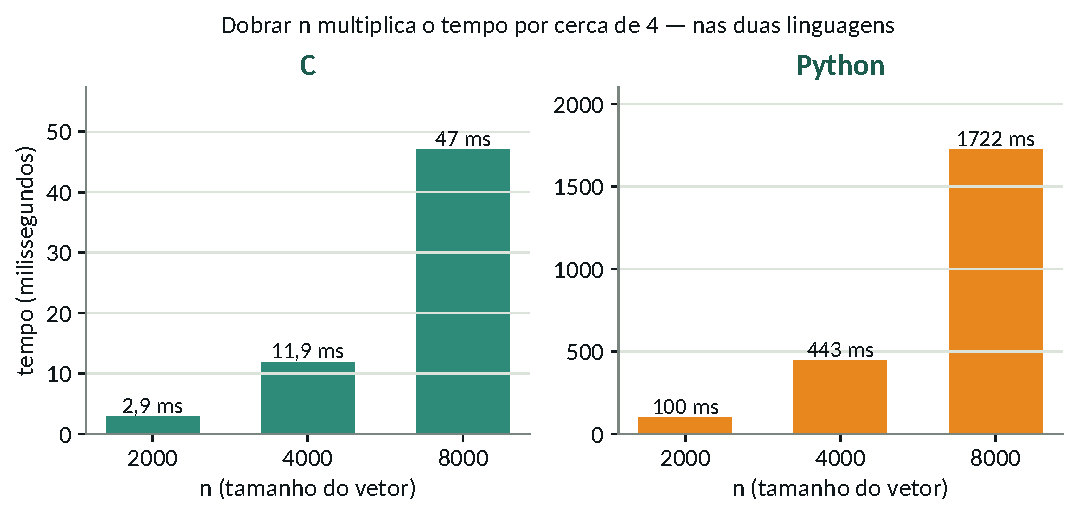
\includegraphics[width=0.92\textwidth]{figuras/f01_tempos_c_python.pdf}
  \caption{Tempo do mesmo algoritmo em C e em Python, para vetores de 2.000, 4.000 e 8.000
  elementos. Repare nas escalas: o Python é cerca de 35 vezes mais lento.}
\end{figure}

\begin{center}
\begin{tabularx}{0.8\textwidth}{L C C C}
\cab \tcx{$n$} & \tc{2.000} & \tc{4.000} & \tc{8.000} \\
Tempo em C & 2,9 ms & 11,9 ms & 47,0 ms \\
\rowcolor{edfundo} Tempo em Python & 100 ms & 443 ms & 1.722 ms \\
\textbf{Quanto multiplicou ao dobrar n} & — & $\approx 4\times$ & $\approx 4\times$ \\
\end{tabularx}
\end{center}

Os números absolutos são muito diferentes: 47 milissegundos contra quase 2 segundos. Mas o
\textbf{comportamento} é o mesmo nas duas linguagens: cada vez que $n$ dobra, o tempo fica cerca
de 4 vezes maior. Essa é a informação que vale em qualquer máquina e em qualquer linguagem — e é
ela que a análise de algoritmos captura.

\begin{atencao}
Os tempos da tabela vão mudar no seu computador. O \enquote{multiplicou por 4} não vai. É por
isso que, em vez de segundos, vamos medir algoritmos pelo \textbf{número de passos} e, mais
ainda, pela \textbf{forma como esse número cresce}.
\end{atencao}

\section{A ideia central: contar passos}

Em vez de cronometrar, vamos \textbf{contar} quantas operações simples o algoritmo executa em
função do tamanho da entrada, que chamaremos de $n$. O resultado é uma função, que escrevemos
como $T(n)$ — lê-se \enquote{tê de ene}. Por exemplo:

\begin{itemize}
  \item \codigo{soma_com_laco} faz um número de passos proporcional a $n$;
  \item \codigo{soma_com_formula} faz sempre o mesmo número de passos, não importa $n$.
\end{itemize}

Contar passos não depende da máquina: um computador mais rápido executa cada passo mais
depressa, mas a quantidade de passos é a mesma. No capítulo 2 você vai aprender a fazer essa
contagem com precisão, e nos capítulos seguintes, a resumir o resultado com as notações $O$,
$\Omega$ e $\Theta$.

\section{O caminho desta apostila}

\begin{center}
\begin{tabularx}{\textwidth}{P{3.2cm} L}
\cab \tc{Capítulos} & \tc{O que você vai aprender} \\
2 & contar os passos de um algoritmo e escrever $T(n)$ \\
\rowcolor{edfundo} 3 e 4 & a matemática necessária, do zero: funções, potências, logaritmos, somatórios, termo dominante \\
5, 6 e 7 & as notações $O$ (teto), $\Omega$ (piso) e $\Theta$ (justo) \\
\rowcolor{edfundo} 8 e 9 & melhor, pior e caso médio — com o Insertion Sort como estudo de caso \\
10 e 11 & comparar famílias de funções e usar derivadas para entender o crescimento \\
\rowcolor{edfundo} 12 e 13 & regras práticas para analisar código e a revisão das Aulas 1 a 3 \\
14 & o Campo Minado: regras, técnicas e análise de custo \\
\rowcolor{edfundo} 15 e 16 & lista de exercícios resolvidos e resumo para a prova \\
\end{tabularx}
\end{center}

\begin{exrapido}
Para $n = 1.000.000$, quantas somas \codigo{soma_com_laco} faz? E quantas contas faz
\codigo{soma_com_formula}? Se cada conta levasse 1 microssegundo, quanto tempo cada uma
levaria?
\end{exrapido}

\begin{respostas}
  \resp{1.1} \codigo{soma_com_laco} faz 1.000.000 de somas (uma por número), ou seja, cerca de
  1 segundo a 1 microssegundo por soma. \codigo{soma_com_formula} faz sempre 3 contas: cerca de
  3 microssegundos. E se $n$ fosse um bilhão, a primeira levaria uns 17 minutos; a segunda,
  os mesmos 3 microssegundos.
\end{respostas}

% =====================================================================
\chapter{Contando operações}\label{cap:02}
\naaula{06 a 08}

Neste capítulo vamos transformar um trecho de código em uma função $T(n)$: o número de passos
que ele executa para uma entrada de tamanho $n$.

\section{O modelo de custo}

Precisamos combinar o que conta como \enquote{um passo}. Usaremos um modelo simples, que é o
mesmo dos slides e dos programas da aula:

\begin{center}
\begin{tabularx}{0.92\textwidth}{L L}
\cab \tc{Custa 1 passo cada vez que executa} & \tc{Exemplo} \\
uma atribuição & \codigo{total = 0} \\
\rowcolor{edfundo} um teste de laço ou de \codigo{if} & \codigo{i < n}, \codigo{v[i] == valor} \\
um incremento & \codigo{i++}, \codigo{i = i + 1} \\
\rowcolor{edfundo} um comando simples do corpo & \codigo{total = total + v[i]} \\
um \codigo{return} & \codigo{return total} \\
\end{tabularx}
\end{center}

\begin{intuicao}
Na vida real, \codigo{total = total + v[i]} envolve várias operações da máquina (ler
\codigo{v[i]}, somar, guardar). Contar isso como 1 passo parece grosseiro, mas não faz diferença
no que nos interessa: se cada \enquote{passo} na verdade custar 3 operações, o total só fica
multiplicado por 3 — e, como você verá no capítulo 4, constantes multiplicativas não mudam a
forma como o custo cresce.
\end{intuicao}

O segredo da contagem é perguntar, para cada linha: \textbf{quantas vezes ela executa?}
Multiplicamos o custo da linha por esse número e somamos tudo.

\section{Exemplo 1: somar um vetor}

\begin{lstlisting}[style=c]
int soma(const int v[], int n) {
    int total = 0;                 /* custo 1, executa 1 vez           */
    for (int i = 0; i < n; i++) {  /* i = 0: 1 vez | i < n: n + 1 vezes | i++: n vezes */
        total = total + v[i];      /* custo 1, executa n vezes         */
    }
    return total;                  /* custo 1, executa 1 vez           */
}
\end{lstlisting}

\begin{center}
\begin{tabularx}{0.9\textwidth}{L C C}
\cab \tc{Linha} & \tc{Vezes} & \tc{Passos} \\
\codigo{int total = 0;} & 1 & 1 \\
\rowcolor{edfundo} \codigo{int i = 0} & 1 & 1 \\
\codigo{i < n} & $n + 1$ & $n + 1$ \\
\rowcolor{edfundo} \codigo{total = total + v[i];} & $n$ & $n$ \\
\codigo{i++} & $n$ & $n$ \\
\rowcolor{edfundo} \codigo{return total;} & 1 & 1 \\
\textbf{Total} & & $\mathbf{3n + 4}$ \\
\end{tabularx}
\end{center}

Por que o teste \codigo{i < n} executa $n + 1$ vezes, e não $n$? Porque ele é avaliado uma vez
para cada volta do laço (dando verdadeiro) e \textbf{mais uma vez no final}, quando dá falso e o
laço termina. Esse \enquote{mais um} é o detalhe que mais gente esquece.

\begin{center}
\begin{tabularx}{0.7\textwidth}{C C}
\cab \tcx{$n$} & \tcx{$T(n) = 3n + 4$} \\
10 & 34 \\
\rowcolor{edfundo} 100 & 304 \\
1.000 & 3.004 \\
\end{tabularx}
\end{center}

Em Python, o mesmo cálculo pode ser escrito com \codigo{while}, deixando cada passo visível.
A contagem é idêntica:

\begin{lstlisting}
def soma(v, n):
    total = 0                 # 1 vez
    i = 0                     # 1 vez
    while i < n:              # n + 1 vezes
        total = total + v[i]  # n vezes
        i = i + 1             # n vezes
    return total              # 1 vez
\end{lstlisting}

\begin{dica}
O programa \codigo{python/contagem_operacoes.py} (e a versão em C) conta os passos de verdade,
com um contador, e compara com a fórmula $3n + 4$. Rode e confira que os números batem.
\end{dica}

\section{Exemplo 2: busca linear}

Esta é a mesma lógica do \codigo{lista_buscar()} da Aula 1: procurar um valor olhando as
posições uma a uma.

\begin{lstlisting}[style=c]
int buscar(const int dados[], int tamanho, int valor) {
    for (int i = 0; i < tamanho; i++) {
        if (dados[i] == valor) {
            return i;
        }
    }
    return -1;
}
\end{lstlisting}

Agora aparece uma novidade: o número de passos \textbf{depende dos dados}, e não só de $n$.

\begin{itemize}
  \item \textbf{Valor ausente (pior situação):} o laço dá todas as voltas. São 1 passo para
        \codigo{i = 0}, $n + 1$ testes \codigo{i < n}, $n$ comparações no \codigo{if}, $n$
        incrementos e 1 \codigo{return -1}: $T(n) = 3n + 3$. Para $n = 100$, 303 passos.
  \item \textbf{Valor na posição 0 (melhor situação):} \codigo{i = 0}, um teste, uma comparação
        e o \codigo{return}: $T(n) = 4$, qualquer que seja $n$.
\end{itemize}

Essa diferença entre \enquote{melhor} e \enquote{pior} situação é tão importante que ganha um
capítulo inteiro, o 8.

\section{Exemplo 3: laços aninhados}

O que acontece com um laço dentro de outro? Este trecho imprime todos os pares $(i, j)$:

\begin{lstlisting}[style=c]
for (int i = 0; i < n; i++) {
    for (int j = 0; j < n; j++) {
        printf("%d %d\n", i, j);
    }
}
\end{lstlisting}

O laço de fora faz o de sempre: 1 inicialização, $n + 1$ testes e $n$ incrementos. O de dentro
\textbf{roda inteiro a cada volta} do de fora, ou seja, $n$ vezes:

\begin{center}
\begin{tabularx}{0.9\textwidth}{L C}
\cab \tc{Linha} & \tc{Vezes} \\
\codigo{int i = 0} ; \codigo{i < n} ; \codigo{i++} & $1 + (n+1) + n$ \\
\rowcolor{edfundo} \codigo{int j = 0} (uma vez por volta de fora) & $n$ \\
\codigo{j < n} ($n + 1$ por volta de fora) & $n(n + 1) = n^2 + n$ \\
\rowcolor{edfundo} \codigo{j++} e \codigo{printf} ($n$ cada, por volta de fora) & $n^2 + n^2$ \\
\textbf{Total} & $\mathbf{3n^2 + 4n + 2}$ \\
\end{tabularx}
\end{center}

Um laço dentro de outro \textbf{multiplica}: $n$ voltas de fora $\times$ $n$ voltas de dentro dão
$n^2$ execuções do corpo. Guarde essa ideia; ela volta no capítulo 12.

\section{Exemplo 4: um laço que divide por 2}

\begin{lstlisting}
i = n
while i > 1:
    i = i // 2      # divisão inteira por 2
\end{lstlisting}

Com $n = 16$, \codigo{i} vale 16, 8, 4, 2 e 1: o corpo executa 4 vezes, e o teste
\codigo{i > 1}, 5 vezes. Total: $1 + 5 + 4 = 10$ passos. Com $n = 1.024$, seriam só 10
divisões. Esse \enquote{quantas vezes dá para dividir ao meio} tem nome — é o
\textbf{logaritmo}, assunto da seção~3.4. O custo deste laço é $T(n) = 2\log_2 n + 2$.

\section{Cuidado com o Python: uma linha não é um passo}

Linguagens como Python escondem laços dentro de operações que parecem simples. No nosso modelo,
uma linha só vale 1 passo se ela realmente fizer uma quantidade fixa de trabalho.

\begin{center}
\begin{tabularx}{\textwidth}{P{4.4cm} C L}
\cab \tc{Operação em Python} & \tc{Custo} & \tc{Por quê} \\
\codigo{v[i]}, \codigo{len(v)} & $O(1)$ & lista contígua: acesso direto (Aula 1) \\
\rowcolor{edfundo} \codigo{v.append(x)} & $O(1)$\,* & escreve no fim; às vezes realoca (Aula 1) \\
\codigo{x in v} & $O(n)$ & percorre a lista procurando \codigo{x} \\
\rowcolor{edfundo} \codigo{v.insert(0, x)} & $O(n)$ & desloca todos os elementos (Aula 1) \\
\codigo{v.remove(x)}, \codigo{v.index(x)} & $O(n)$ & procura e depois desloca \\
\rowcolor{edfundo} \codigo{min(v)}, \codigo{max(v)}, \codigo{sum(v)} & $O(n)$ & olham todos os elementos \\
\codigo{v.pop()} & $O(1)$ & remove do fim, como o desempilhar (Aula 2) \\
\end{tabularx}
\end{center}

{\small * Em média. De vez em quando, a lista precisa de mais espaço e é copiada inteira, mas
isso é raro o suficiente para, na média, cada \codigo{append} custar um número fixo de passos.}

\begin{atencao}
\codigo{if valor in lista:} parece um único teste, mas é uma busca linear inteira! Foi por isso
que, na Aula 3, o \codigo{pertence()} do nosso Conjunto era $O(n)$. Se essa linha estiver dentro
de um laço de $n$ voltas, o total vira $n \times n = n^2$.
\end{atencao}

\begin{exrapido}[22]
Conte os passos da função abaixo, que devolve o maior valor de um vetor com $n \ge 1$
elementos. (a) Quantos passos, se o maior valor estiver na posição 0? (b) E se o vetor
estiver em ordem crescente, fazendo \codigo{m = v[i]} executar em todas as voltas?

\begin{lstlisting}[style=c]
int maior(const int v[], int n) {
    int m = v[0];
    for (int i = 1; i < n; i++) {
        if (v[i] > m) {
            m = v[i];
        }
    }
    return m;
}
\end{lstlisting}
\end{exrapido}

\begin{exrapido}
Na busca linear com o valor ausente e $n = 50$: (a) quantas vezes o \codigo{if} é avaliado?
(b) quantos passos ao todo?
\end{exrapido}

\begin{respostas}
  \resp{2.1} Repare que o laço começa em \codigo{i = 1}: ele dá $n - 1$ voltas e o teste
  \codigo{i < n} executa $n$ vezes. Contando: \codigo{m = v[0]} (1) + \codigo{i = 1} (1) +
  testes ($n$) + \codigo{if} ($n - 1$) + incrementos ($n - 1$) + \codigo{return} (1).
  (a) Sem nenhuma troca de \codigo{m}: $1 + 1 + n + (n-1) + (n-1) + 1 = 3n + 1$.
  (b) Com \codigo{m = v[i]} executando em todas as $n - 1$ voltas: $3n + 1 + (n - 1) = 4n$.
  Nos dois casos, o custo cresce proporcionalmente a $n$.
  \resp{2.2} (a) 50 vezes, uma por posição. (b) $3 \cdot 50 + 3 = 153$ passos.
\end{respostas}

% =====================================================================
\chapter{Matemática de bolso}\label{cap:03}
\naaula{09 a 16}

Este capítulo reúne toda a matemática de que você vai precisar, explicada do zero. Não pule
nenhuma seção, mesmo que o assunto pareça conhecido: cada uma termina ligando a ideia a algo que
você já programou.

% ---------------------------------------------------------------------
\section{Funções: uma máquina de entrada e saída}

Uma \textbf{função} é uma regra que recebe um valor de entrada e devolve um valor de saída. Pense
numa máquina: você coloca um número de um lado e sai um número do outro.

\begin{figure}[!htb]
\centering
\begin{tikzpicture}[font=\large]
  \node[draw=edteal, fill=edtealclaro, line width=1.2pt, rounded corners=3pt,
        minimum width=3.2cm, minimum height=1.4cm] (m) at (0,0) {$T(n) = 3n + 4$};
  \node[anchor=east] (e) at (-3.4,0) {$n = 5$};
  \node[anchor=west] (s) at (3.4,0) {$T(5) = 19$};
  \draw[-{Latex[length=3mm]}, line width=1.2pt, edverde] (e) -- (m);
  \draw[-{Latex[length=3mm]}, line width=1.2pt, edlaranja] (m) -- (s);
  \node[font=\small, color=edcinza] at (-2.6,-1.0) {entrada: o tamanho};
  \node[font=\small, color=edcinza] at (2.8,-1.0) {saída: os passos};
\end{tikzpicture}
\caption{A função $T(n) = 3n + 4$, que conta os passos da soma de um vetor (capítulo 2).}
\end{figure}

Escrevemos $T(n)$ para dizer \enquote{o valor de $T$ quando a entrada é $n$}. Para calcular, basta
trocar $n$ pelo número: $T(5) = 3 \cdot 5 + 4 = 19$. Em análise de algoritmos, a entrada $n$ é
quase sempre o \textbf{tamanho} dos dados — o mesmo número que o \codigo{tamanho()} da nossa Lista
devolve — e a saída é o \textbf{custo}: passos, comparações, deslocamentos.

\subsection{Tabela e gráfico}

Uma função pode ser mostrada como tabela ou como gráfico. No gráfico, cada ponto tem duas
coordenadas: a posição na horizontal é a entrada $n$; a altura é a saída $T(n)$.

\begin{center}
\begin{tabularx}{0.85\textwidth}{P{3.2cm} C C C C C C}
\cab \tcx{$n$} & \tc{0} & \tc{1} & \tc{2} & \tc{5} & \tc{8} & \tc{10} \\
$T(n) = 3n + 4$ & 4 & 7 & 10 & 19 & 28 & 34 \\
\end{tabularx}
\end{center}

\begin{figure}[!htb]
  \centering
  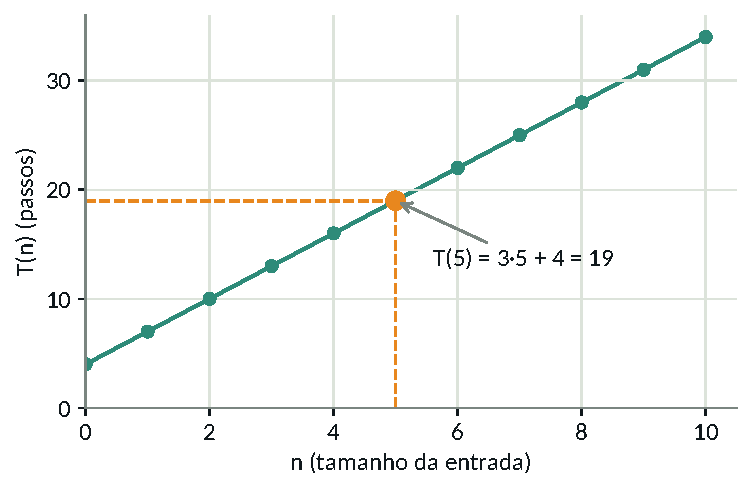
\includegraphics[width=0.66\textwidth]{figuras/f03_grafico_3n4.pdf}
  \caption{Como ler um gráfico: ande na horizontal até $n = 5$, suba até a linha e olhe a altura
  à esquerda: 19.}
\end{figure}

% ---------------------------------------------------------------------
\section{Funções crescentes}

Uma função é \textbf{crescente} quando, ao aumentar a entrada, a saída nunca diminui. Em
símbolos: se $a < b$, então $f(a) \le f(b)$. O custo de um algoritmo é (quase sempre) uma função
crescente: mais dados, mais trabalho. O que muda de um algoritmo para outro é \textbf{a
velocidade} com que o custo cresce.

\begin{figure}[!htb]
  \centering
  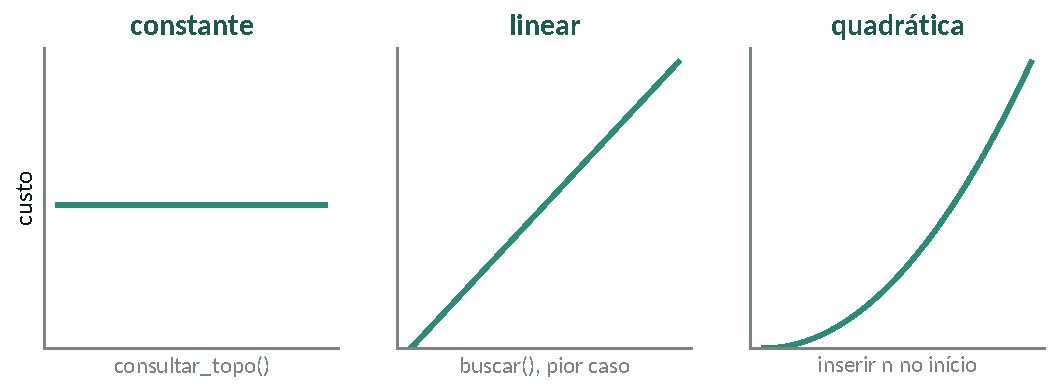
\includegraphics[width=0.95\textwidth]{figuras/f03_tipos_crescimento.pdf}
  \caption{Três formas de crescer, com exemplos das Aulas 1 e 2.}
\end{figure}

\begin{itemize}
  \item \textbf{Constante:} o custo não depende de $n$. O \codigo{consultar_topo()} da Pilha
        custa o mesmo com 3 ou com 3 milhões de elementos. (Uma função constante conta como
        crescente no sentido de que \enquote{nunca diminui}.)
  \item \textbf{Linear:} o custo cresce na mesma proporção de $n$. Dobrou $n$, dobrou o custo.
        É o caso da busca linear quando o valor não está na lista.
  \item \textbf{Quadrática:} o custo cresce muito mais rápido. Dobrou $n$, o custo
        quadruplica. É o caso de inserir $n$ elementos, um a um, no início de uma lista contígua.
\end{itemize}

\begin{exrapido}
Considere $f(n) = 7$, $g(n) = 2n + 1$ e $h(n) = n^2$. (a) Calcule as três para $n = 1$, $5$ e
$10$. (b) Em cada caso, qual é a maior? (c) O que isso sugere sobre comparar funções olhando só
valores pequenos de $n$?
\end{exrapido}

% ---------------------------------------------------------------------
\section{Potências e raízes}

A \textbf{potência} $n^k$ é $n$ multiplicado por ele mesmo $k$ vezes: $n^2 = n \cdot n$ (lê-se
\enquote{ene ao quadrado}) e $n^3 = n \cdot n \cdot n$ (\enquote{ene ao cubo}). Os nomes vêm da
geometria: $n^2$ é a área de um quadrado de lado $n$; $n^3$, o volume de um cubo.

\begin{figure}[!htb]
\centering
\begin{tikzpicture}[scale=0.55]
  \foreach \x in {0,...,3} \foreach \y in {0,...,3}
    \draw[fill=edtealclaro, draw=edteal, line width=0.8pt] (\x,\y) rectangle ++(1,1);
  \node[font=\small] at (2,-0.6) {lado $n = 4$};
  \node[font=\small, rotate=90] at (-0.6,2) {lado $n = 4$};
  \node[font=\large, anchor=west] at (4.8,2.6) {$n^2 = 4 \times 4 = 16$ casas};
  \node[font=\small, anchor=west, color=edcinza, align=left] at (4.8,1.2)
    {como um tabuleiro de Campo Minado $4 \times 4$,\\ou uma matriz guardada numa lista contígua};
\end{tikzpicture}
\caption{$n^2$ conta as casas de um quadrado de lado $n$.}
\end{figure}

A \textbf{raiz quadrada} faz o caminho inverso: $\sqrt{n}$ é o lado de um quadrado com $n$ casas.
$\sqrt{16} = 4$, $\sqrt{100} = 10$, $\sqrt{10.000} = 100$. Também se escreve $\sqrt{n} = n^{1/2}$.

\subsection{Regras que vamos usar}

\begin{center}
\begin{tabularx}{\textwidth}{P{3.6cm} P{3.8cm} L}
\cab \tc{Regra} & \tc{Exemplo} & \tc{Em palavras} \\
$n^a \cdot n^b = n^{a+b}$ & $2^3 \cdot 2^4 = 2^7 = 128$ & multiplicar: soma os expoentes \\
\rowcolor{edfundo} $(n^a)^b = n^{a \cdot b}$ & $(n^2)^3 = n^6$ & potência de potência: multiplica \\
$n^1 = n$ \quad e \quad $n^0 = 1$ & $7^0 = 1$ & qualquer número (não nulo) elevado a 0 dá 1 \\
\rowcolor{edfundo} $n^{-1} = \dfrac{1}{n}$ & $10^{-2} = \dfrac{1}{100}$ & expoente negativo: inverte \\
$n^{1/2} = \sqrt{n}$ & $64^{1/2} = 8$ & expoente ½ é a raiz quadrada \\
\end{tabularx}
\end{center}

\begin{conexao}
Na Aula 3, a interseção \enquote{ingênua} de dois Conjuntos com $n$ e $m$ elementos perguntava,
para cada elemento do primeiro, se ele pertencia ao segundo: $n$ consultas de custo $m$, ou
seja, $n \cdot m$ comparações. Se os dois têm o mesmo tamanho, isso dá $n^2$.
\end{conexao}

\begin{exrapido}
Calcule: (a) $2^3 \cdot 2^4$; (b) $\sqrt{64}$; (c) $(n^2)^3$; (d) $10^{-2}$; (e) $1.000^{1/3}$
(dica: que número multiplicado por ele mesmo 3 vezes dá 1.000?).
\end{exrapido}

% ---------------------------------------------------------------------
\section{Logaritmos: quantas vezes dá para dividir ao meio?}

Pegue 16 caixas e vá dividindo ao meio até sobrar uma. Quantas divisões são necessárias?

\begin{figure}[!htb]
\centering
\begin{tikzpicture}[scale=0.42]
  \foreach \linha/\qtd in {0/16, 1/8, 2/4, 3/2, 4/1} {
    \foreach \i in {1,...,\qtd}
      \draw[fill=edtealclaro, draw=edteal, line width=0.7pt] (\i-1, -\linha*1.5) rectangle ++(0.85,0.85);
    \node[anchor=west, font=\small] at (16.4, -\linha*1.5+0.42) {\textbf{\qtd}};
  }
  \foreach \linha/\num in {0/1, 1/2, 2/3, 3/4}
    \node[font=\small, color=edlaranja, anchor=west] at (18.4, -\linha*1.5-0.33) {$\div 2$ \ (divisão \num)};
\end{tikzpicture}
\caption{$16 \to 8 \to 4 \to 2 \to 1$: são 4 divisões. Por isso, $\log_2 16 = 4$.}
\end{figure}

O número de divisões ao meio até chegar a 1 é o \textbf{logaritmo na base 2}. Escrevemos
$\log_2 16 = 4$ (lê-se \enquote{logaritmo de 16 na base 2 é 4}). Olhando ao contrário: dobrando
4 vezes a partir de 1, chegamos a 16, ou seja, $2^4 = 16$. Esta é a definição:

\begin{center}
\colorbox{edtealclaro}{\large\quad $\log_2 n = x \quad\Longleftrightarrow\quad 2^x = n$\quad}
\end{center}

\begin{center}
\begin{tabularx}{\textwidth}{L C C C C C C C}
\cab \tcx{$n$} & \tc{1} & \tc{2} & \tc{8} & \tc{16} & \tc{1.024} & \tc{1.048.576} & \tc{≈ 1 bilhão} \\
$\log_2 n$ & 0 & 1 & 3 & 4 & 10 & 20 & $\approx 30$ \\
\end{tabularx}
\end{center}

Repare no mais importante: quando $n$ vai de mil para um milhão (mil vezes mais), o logaritmo só
vai de 10 para 20. \textbf{O logaritmo cresce muito devagar.} Um algoritmo que faz $\log_2 n$
passos é excelente.

\begin{intuicao}
O jogo \enquote{adivinhe o número de 1 a 100}: a cada palpite, você ouve \enquote{maior} ou
\enquote{menor}. Chutando sempre o meio, cada resposta elimina metade dos números que sobram. Em
no máximo 7 palpites você acerta, porque $2^7 = 128 \ge 100$. Esse é o princípio da
\emph{busca binária} em um vetor ordenado: cerca de $\log_2 n$ comparações.
\end{intuicao}

\subsection{E quando \texorpdfstring{$n$}{n} não é uma potência de 2?}

O logaritmo continua existindo, só que não é inteiro: $\log_2 1.000 \approx 9{,}97$, porque
$2^{9{,}97} \approx 1.000$. Para calcular numa calculadora (ou no Python), use:

\[
\log_2 n = \frac{\ln n}{\ln 2} \approx 3{,}32 \cdot \log_{10} n
\qquad\text{no Python: } \texttt{math.log2(n)}
\]

\subsection{Propriedades úteis}

\begin{center}
\begin{tabularx}{\textwidth}{P{4.2cm} P{4.4cm} L}
\cab \tc{Propriedade} & \tc{Exemplo} & \tc{Em palavras} \\
$\log(a \cdot b) = \log a + \log b$ & $\log_2 (8 \cdot 4) = 3 + 2 = 5$ & produto vira soma \\
\rowcolor{edfundo} $\log(n^k) = k \cdot \log n$ & $\log_2 (2^{10}) = 10$ & o expoente \enquote{desce} \\
$\log 1 = 0$ & $\log_2 1 = 0$ & porque $2^0 = 1$ \\
\rowcolor{edfundo} $\log_2 n = 3{,}32 \cdot \log_{10} n$ & $\log_2 1.000 \approx 3{,}32 \cdot 3$ & bases diferentes só diferem por uma constante \\
\end{tabularx}
\end{center}

\begin{atencao}
A última propriedade tem uma consequência importante: em análise de algoritmos, a base do
logaritmo \textbf{não importa}. Trocar de base só multiplica o resultado por uma constante — e
constantes são desprezadas (capítulo 4). Por isso escrevemos simplesmente $O(\log n)$.
\end{atencao}

\begin{figure}[!htb]
  \centering
  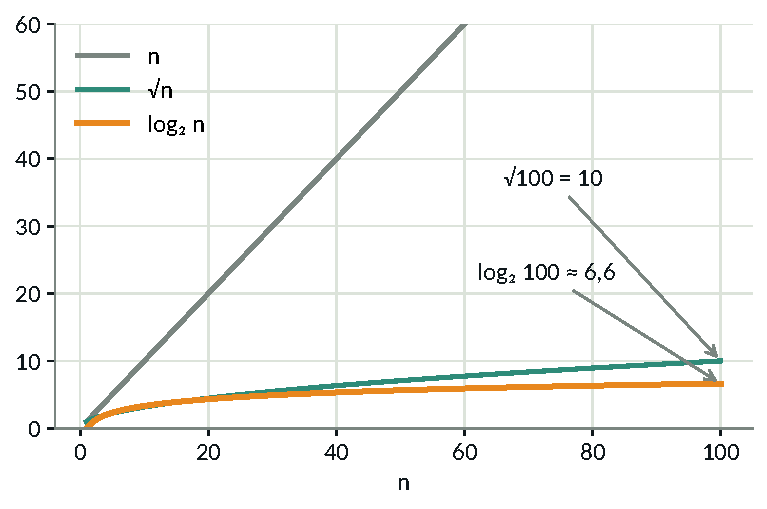
\includegraphics[width=0.7\textwidth]{figuras/f03_log_raiz.pdf}
  \caption{Para $n = 100$: $n$ vale 100, $\sqrt{n}$ vale 10 e $\log_2 n$ vale só 6,6.}
\end{figure}

\begin{exrapido}
(a) $\log_2 64$; (b) $\log_2 1.024$; (c) entre quais inteiros está $\log_2 100$?
(d) Quantas vezes é preciso dividir 1.000.000 ao meio para chegar a 1 (aproximadamente)?
\end{exrapido}

% ---------------------------------------------------------------------
\section{Exponenciais: dobrar a cada passo}

Na \textbf{exponencial} $2^n$, a variável está no expoente: cada vez que $n$ aumenta 1, o valor
\textbf{dobra}. $2^{10} = 1.024$, $2^{20} \approx$ um milhão, $2^{30} \approx$ um bilhão.

\begin{intuicao}
Diz a lenda que o inventor do xadrez pediu como prêmio 1 grão de trigo na primeira casa do
tabuleiro, 2 na segunda, 4 na terceira, dobrando até a casa 64. Parece pouco, mas a última casa
sozinha teria $2^{63}$ grãos, e o total, $2^{64} - 1 \approx 1{,}8 \times 10^{19}$ grãos —
muito mais trigo do que o mundo inteiro já produziu.
\end{intuicao}

Onde a exponencial aparece em computação? Sempre que um algoritmo testa \textbf{todas as
combinações} de escolhas do tipo sim/não.

\begin{conexao}
Um Conjunto (Aula 3) com $n$ elementos tem $2^n$ subconjuntos. Para cada elemento, há duas
escolhas: ele está no subconjunto ou não. São $2 \times 2 \times \dots \times 2 = 2^n$ combinações.
Para $\{A, B, C\}$:

\begin{center}
\begin{tabularx}{0.9\linewidth}{C C C L}
\cab \tc{A está?} & \tc{B está?} & \tc{C está?} & \tc{Subconjunto} \\
não & não & não & $\varnothing$ (vazio) \\
\rowcolor{white} não & não & sim & $\{C\}$ \\
não & sim & não & $\{B\}$ \\
\rowcolor{white} não & sim & sim & $\{B, C\}$ \\
sim & não & não & $\{A\}$ \\
\rowcolor{white} sim & não & sim & $\{A, C\}$ \\
sim & sim & não & $\{A, B\}$ \\
\rowcolor{white} sim & sim & sim & $\{A, B, C\}$ \\
\end{tabularx}
\end{center}

São $2^3 = 8$ subconjuntos. Com 30 elementos, seriam mais de um bilhão.
\end{conexao}

\begin{figure}[!htb]
  \centering
  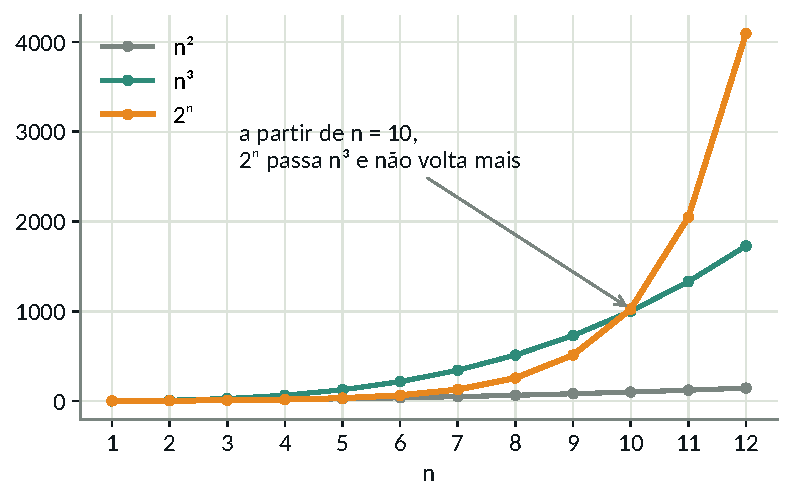
\includegraphics[width=0.7\textwidth]{figuras/f03_exponencial.pdf}
  \caption{No começo, $2^n$ parece inofensiva: fica abaixo de $n^3$ até $n = 9$. A partir de
  $n = 10$, passa à frente e dispara.}
\end{figure}

% ---------------------------------------------------------------------
\section{Fatorial: todas as ordens possíveis}

O \textbf{fatorial} de $n$, escrito $n!$ (lê-se \enquote{ene fatorial}), é o produto de todos os
inteiros de 1 até $n$:
\[
n! = n \times (n-1) \times \dots \times 2 \times 1,
\qquad 3! = 3 \cdot 2 \cdot 1 = 6, \qquad 5! = 120, \qquad 0! = 1 \text{ (por convenção)}.
\]

O fatorial conta de quantas \textbf{ordens} diferentes podemos arrumar $n$ objetos.

\begin{conexao}
Na central de impressão da Aula 2, três trabalhos — 101, 102 e 103 — podem chegar à fila em
qualquer ordem. Para o primeiro lugar, há 3 opções; escolhido o primeiro, sobram 2 para o
segundo; e o último fica com a única que resta: $3 \times 2 \times 1 = 6$ ordens.
\end{conexao}

\begin{figure}[!htb]
\centering
\begin{tikzpicture}[
  level 1/.style={sibling distance=4.4cm, level distance=1.25cm},
  level 2/.style={sibling distance=2.1cm, level distance=1.25cm},
  level 3/.style={level distance=1.1cm},
  every node/.style={font=\small, draw=edteal, fill=edtealclaro, rounded corners=2pt, inner sep=3pt},
  edge from parent/.style={draw=edteal, line width=0.8pt}]
  \node[fill=edteal, text=white] {início}
    child {node {101}
      child {node {102} child {node[fill=white] {103}}}
      child {node {103} child {node[fill=white] {102}}}}
    child {node {102}
      child {node {101} child {node[fill=white] {103}}}
      child {node {103} child {node[fill=white] {101}}}}
    child {node {103}
      child {node {101} child {node[fill=white] {102}}}
      child {node {102} child {node[fill=white] {101}}}};
\end{tikzpicture}
\caption{As $3! = 6$ ordens de chegada de três trabalhos à fila de impressão. Cada caminho do
início até uma folha é uma ordem.}
\end{figure}

\begin{center}
\begin{tabularx}{\textwidth}{L C C C C C}
\cab \tcx{$n$} & \tc{3} & \tc{5} & \tc{10} & \tc{15} & \tc{20} \\
$2^n$ & 8 & 32 & 1.024 & 32.768 & $\approx 1$ milhão \\
\rowcolor{edfundo} $n!$ & 6 & 120 & 3.628.800 & $\approx 1{,}3 \times 10^{12}$ & $\approx 2{,}4 \times 10^{18}$ \\
\end{tabularx}
\end{center}

O fatorial cresce ainda mais rápido que a exponencial: a partir de $n = 4$ ($4! = 24 > 2^4 = 16$),
passa à frente e nunca mais é alcançado. Um algoritmo que testa todas as ordens possíveis de $n$
itens é inviável já para $n$ em torno de 20.

\begin{exrapido}
(a) Liste os subconjuntos de $\{A, B, C\}$ sem olhar a tabela. (b) Calcule $4!$. (c) De quantas
formas 4 trabalhos podem chegar à fila? (d) Calcule $\dfrac{5!}{3!}$ sem calcular os fatoriais
inteiros.
\end{exrapido}

% ---------------------------------------------------------------------
\section{Somatórios e a soma de Gauss}

Muitos algoritmos fazem um trabalho que cresce a cada volta de um laço: 1 passo na primeira volta,
2 na segunda, 3 na terceira\dots\ Para somar isso tudo, usamos o \textbf{somatório}, escrito com a
letra grega $\Sigma$ (sigma maiúsculo):

\[
\sum_{i=1}^{n} i \;=\; 1 + 2 + 3 + \dots + n
\]

Leia assim: \enquote{a soma de $i$, para $i$ indo de 1 até $n$}. O número embaixo diz onde o
contador começa; o de cima, onde termina; e a expressão ao lado diz o que somar em cada volta —
exatamente como um laço \codigo{for}:

\begin{lstlisting}
total = 0
for i in range(1, n + 1):   # i vai de 1 até n
    total = total + i       # soma a expressão "i"
\end{lstlisting}

Mais exemplos: $\sum_{i=1}^{4} i = 1 + 2 + 3 + 4 = 10$ \quad e \quad
$\sum_{i=1}^{3} 2i = 2 + 4 + 6 = 12$.

\subsection{O truque de Gauss}

Conta-se que, criança, Carl Friedrich Gauss recebeu a tarefa de somar os números de 1 a 100 e
respondeu em segundos: 5.050. Ele percebeu que, escrevendo a soma de trás para a frente embaixo
dela mesma, cada coluna soma sempre 101:

\[
\begin{array}{r@{\;}c@{\;}c@{\;}c@{\;}c@{\;}c@{\;}c@{\;}c@{\;}c}
      & 1   & + & 2   & + & \cdots & + & 100 & \\
  +   & 100 & + & 99  & + & \cdots & + & 1   & \\ \hline
      & 101 & + & 101 & + & \cdots & + & 101 & = 100 \times 101
\end{array}
\]

Isso é o dobro da soma pedida; então a soma é $\dfrac{100 \times 101}{2} = 5.050$. Em geral:

\begin{center}
\colorbox{edtealclaro}{\large\quad $\displaystyle \sum_{i=1}^{n} i \;=\; 1 + 2 + \dots + n \;=\; \frac{n(n+1)}{2}$\quad}
\end{center}

\begin{figure}[!htb]
\centering
\begin{tikzpicture}[scale=0.62]
  \foreach \c in {1,...,5} \foreach \r in {1,...,\c}
    \draw[fill=edtealclaro, draw=edteal, line width=0.8pt] (\c-1, \r-1) rectangle ++(1,1);
  \foreach \c in {1,...,5} \foreach \r in {\c,...,5}
    \draw[fill=edlaranjaclaro, draw=edlaranja, line width=0.8pt] (\c-1, \r) rectangle ++(1,1);
  \node[font=\small] at (2.5,-0.6) {$n = 5$ colunas};
  \node[font=\small, rotate=90] at (-0.7,3) {$n + 1 = 6$ linhas};
  \node[font=\small, anchor=west] at (6.0,4.2) {\textcolor{edteal}{\textbf{escada verde:}} $1 + 2 + 3 + 4 + 5$};
  \node[font=\small, anchor=west] at (6.0,3.2) {\textcolor{edlaranja}{\textbf{escada laranja:}} a mesma, virada};
  \node[font=\small, anchor=west, align=left] at (6.0,1.8) {juntas: retângulo $5 \times 6 = 30$\\uma só: $30 \div 2 = 15$};
\end{tikzpicture}
\caption{A prova visual de Gauss: duas escadas iguais formam um retângulo $n \times (n+1)$.}
\end{figure}

Duas variações que aparecem muito:
\[
\sum_{i=0}^{n-1} i \;=\; 0 + 1 + \dots + (n-1) \;=\; \frac{(n-1)\,n}{2}
\qquad\text{e}\qquad
\sum_{i=1}^{n} c \;=\; c \cdot n \quad \text{(somar a constante } c\text{, } n \text{ vezes).}
\]

\begin{conexao}
Lembra do exercício 3 da Aula 1 (\enquote{contando deslocamentos})? Inserir $n$ elementos, um a
um, sempre no início de uma lista contígua: o primeiro não desloca ninguém; o segundo desloca 1;
o terceiro, 2; \dots; o último, $n - 1$. Total: $0 + 1 + \dots + (n - 1) = \dfrac{n(n-1)}{2}$
deslocamentos. Para $n = 100$, são 4.950.
\end{conexao}

\begin{exrapido}
(a) $1 + 2 + \dots + 100$. (b) Inserindo 10, 20, 30, 40 e 50, sempre no início de uma lista
contígua vazia, quantos deslocamentos ocorrem ao todo? (c) E para $n = 100$ inserções?
(d) Quanto vale $2 + 4 + 6 + \dots + 2n$? (Dica: coloque o 2 em evidência.)
\end{exrapido}

% ---------------------------------------------------------------------
\section{Para \texorpdfstring{$n$}{n} muito grande}

A análise de algoritmos se interessa pelo que acontece quando $n$ fica \textbf{muito grande} —
milhões, bilhões. Escrevemos $n \to \infty$ (lê-se \enquote{ene tende ao infinito}) para dizer
\enquote{$n$ crescendo sem parar}. Veja o que acontece com duas divisões:

\begin{center}
\begin{tabularx}{\textwidth}{P{2.8cm} C C C C}
\cab \tcx{$n$} & \tc{10} & \tc{100} & \tc{1.000} & \tc{1.000.000} \\
$\dfrac{3n + 4}{n}$ & 3,4 & 3,04 & 3,004 & 3,000004 \\
\rowcolor{edfundo} $\dfrac{n^2}{2^n}$ & 0,098 & $\approx 7{,}9 \times 10^{-27}$ & praticamente 0 & praticamente 0 \\
\end{tabularx}
\end{center}

A primeira divisão se aproxima de 3: para $n$ grande, $3n + 4$ se comporta como \enquote{3 vezes
$n$}, e o $+4$ deixa de importar. A segunda se aproxima de 0: $2^n$ cresce tão mais rápido que
$n^2$ fica insignificante perto dela. Dizemos que a primeira \enquote{tende a 3} e a segunda
\enquote{tende a 0}. Essa é a ideia intuitiva de \textbf{limite}, que volta no capítulo 11 — e é
exatamente o que o próximo capítulo explora.

\begin{respostas}
  \resp{3.1} (a) $n = 1$: $f = 7$, $g = 3$, $h = 1$. $n = 5$: $f = 7$, $g = 11$, $h = 25$.
  $n = 10$: $f = 7$, $g = 21$, $h = 100$. (b) Para $n = 1$, a maior é $f$; para $n = 5$ e
  $n = 10$, é $h$. (c) Quem começa na frente pode terminar atrás: comparar algoritmos com $n$
  pequeno engana. O que importa é o comportamento para $n$ grande.

  \begin{center}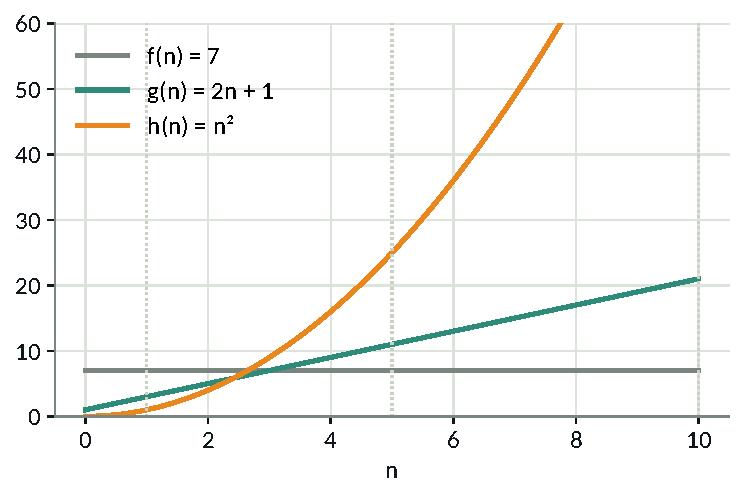
\includegraphics[width=0.6\textwidth]{figuras/f03_fgh.pdf}\end{center}

  \resp{3.2} (a) $2^7 = 128$. (b) 8. (c) $n^6$. (d) $\dfrac{1}{100} = 0{,}01$. (e) 10, porque
  $10 \times 10 \times 10 = 1.000$.
  \resp{3.3} (a) 6, pois $2^6 = 64$. (b) 10. (c) Entre 6 e 7, pois $2^6 = 64 < 100 < 128 = 2^7$
  (o valor exato é $\approx 6{,}64$). (d) Cerca de 20 vezes, pois $2^{20} \approx 1.000.000$.
  \resp{3.4} (a) $\varnothing$, $\{A\}$, $\{B\}$, $\{C\}$, $\{A,B\}$, $\{A,C\}$, $\{B,C\}$ e
  $\{A,B,C\}$: são 8. (b) $4! = 24$. (c) 24 formas. (d) $\dfrac{5 \cdot 4 \cdot 3!}{3!} = 5 \cdot 4 = 20$.
  \resp{3.5} (a) $\dfrac{100 \cdot 101}{2} = 5.050$. (b) $0 + 1 + 2 + 3 + 4 = 10$, que é
  $\dfrac{5 \cdot 4}{2}$. (c) $\dfrac{100 \cdot 99}{2} = 4.950$.
  (d) $2 + 4 + \dots + 2n = 2(1 + 2 + \dots + n) = 2 \cdot \dfrac{n(n+1)}{2} = n(n+1)$.
\end{respostas}

% =====================================================================
\chapter{Termo dominante e análise assintótica}\label{cap:04}
\naaula{17 a 19}

No capítulo 2, a soma de um vetor custou $3n + 4$ passos, e os laços aninhados custaram
$3n^2 + 4n + 2$. Essas fórmulas são exatas, mas têm detalhes demais. Neste capítulo você vai
aprender a ficar só com o que importa.

\section{Quem manda quando \texorpdfstring{$n$}{n} cresce}

Tome $T(n) = 3n^2 + 5n + 2$ e veja quanto cada termo contribui para o total:

\begin{center}
\begin{tabularx}{\textwidth}{L C C C C}
\cab \tcx{$n$} & \tcx{$3n^2$} & \tcx{$5n$} & \tc{2} & \tcx{PARTE DE $3n^2$ NO TOTAL} \\
10 & 300 & 50 & 2 & 85,2\% \\
\rowcolor{edfundo} 100 & 30.000 & 500 & 2 & 98,4\% \\
1.000 & 3.000.000 & 5.000 & 2 & 99,8\% \\
\rowcolor{edfundo} 1.000.000 & $3 \times 10^{12}$ & $5 \times 10^{6}$ & 2 & 99,9998\% \\
\end{tabularx}
\end{center}

\begin{figure}[!htb]
  \centering
  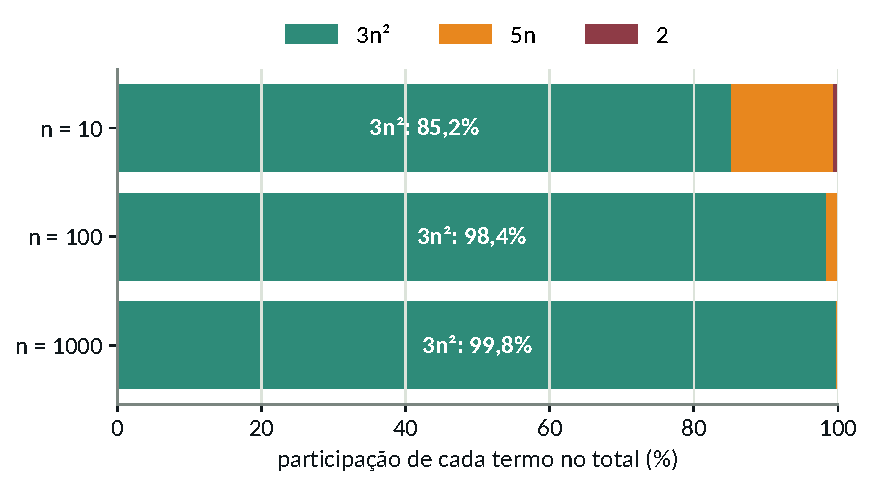
\includegraphics[width=0.74\textwidth]{figuras/f04_termo_dominante.pdf}
  \caption{Quanto maior $n$, mais o termo $3n^2$ domina o total.}
\end{figure}

O termo que cresce mais rápido — aqui, $3n^2$ — acaba respondendo por praticamente todo o custo.
Ele é chamado de \textbf{termo dominante}. Os outros ficam cada vez mais irrelevantes.

\begin{intuicao}
É como comprar um carro e um cafezinho: o preço total é \enquote{o preço do carro}. Ninguém
deixa de comprar o carro por causa do cafezinho. Em $3n^2 + 5n + 2$, o $3n^2$ é o carro.
\end{intuicao}

\section{As duas regras de simplificação}

\begin{enumerate}
  \item \textbf{Fique só com o termo dominante:} $3n^2 + 5n + 2 \;\to\; 3n^2$.
  \item \textbf{Despreze a constante que multiplica:} $3n^2 \;\to\; n^2$.
\end{enumerate}

Dizemos então que $T(n)$ \enquote{cresce como $n^2$}, ou que ele é \enquote{quadrático}.

Por que podemos desprezar a constante? Lembre do capítulo 1: rodar o mesmo algoritmo numa máquina
mais lenta, ou em Python em vez de C, multiplica o tempo por uma constante (ali, cerca de 35).
Constantes mudam de máquina para máquina; a \textbf{forma do crescimento} não muda. Como queremos
uma medida que valha em qualquer máquina, deixamos a constante de lado.

\begin{center}
\begin{tabularx}{0.9\textwidth}{L L L}
\cab \tc{Custo exato} & \tc{Termo dominante} & \tc{Cresce como} \\
$3n + 4$ & $3n$ & $n$ \\
\rowcolor{edfundo} $3n^2 + 4n + 2$ & $3n^2$ & $n^2$ \\
$2\log_2 n + 2$ & $2 \log_2 n$ & $\log n$ \\
\rowcolor{edfundo} $\dfrac{n(n-1)}{2} = \dfrac{n^2}{2} - \dfrac{n}{2}$ & $\dfrac{n^2}{2}$ & $n^2$ \\
$2^n + n^3$ & $2^n$ & $2^n$ \\
\rowcolor{edfundo} $500$ & $500$ & constante \\
\end{tabularx}
\end{center}

\begin{atencao}
Para achar o termo dominante, use a hierarquia do capítulo 3: uma constante cresce menos que
$\log n$, que cresce menos que $n$, que cresce menos que $n^2$, que cresce menos que $2^n$, que
cresce menos que $n!$. Na dúvida, calcule os termos para um $n$ grande, como $n = 1.000$.
\end{atencao}

\section{Análise assintótica}

\textbf{Análise assintótica} é o nome técnico de \enquote{olhar o comportamento quando $n$ fica
muito grande}. A palavra vem de \emph{assíntota}, uma linha da qual uma curva se aproxima cada
vez mais.

Veja por que isso importa. Imagine dois algoritmos: $A$, que faz $100n$ passos, e $B$, que faz
$n^2$. Para $n = 10$, $A$ faz 1.000 passos e $B$ só 100: $B$ parece melhor! Mas:

\begin{figure}[!htb]
  \centering
  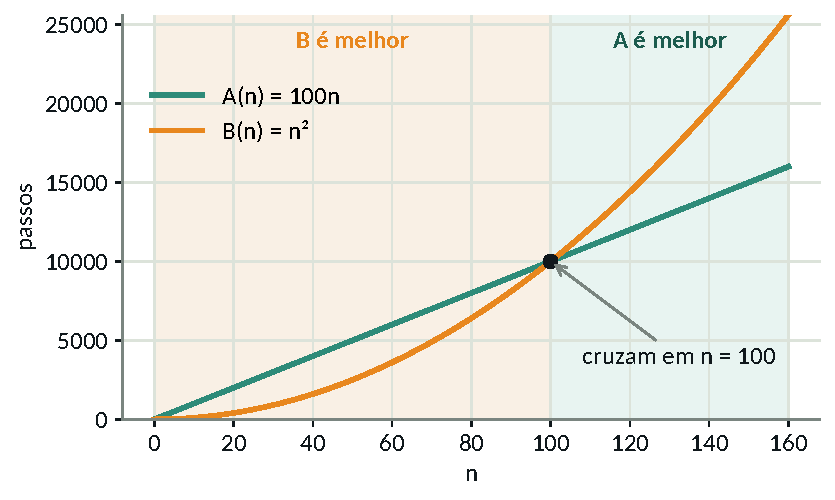
\includegraphics[width=0.72\textwidth]{figuras/f04_cruzamento.pdf}
  \caption{$100n$ e $n^2$ se cruzam em $n = 100$. Depois disso, $A$ ganha, e a vantagem só aumenta.}
\end{figure}

\begin{center}
\begin{tabularx}{\textwidth}{P{2.8cm} C C C C}
\cab \tcx{$n$} & \tc{10} & \tc{100} & \tc{1.000} & \tc{1.000.000} \\
$A(n) = 100n$ & 1.000 & 10.000 & 100.000 & $10^8$ \\
\rowcolor{edfundo} $B(n) = n^2$ & 100 & 10.000 & 1.000.000 & $10^{12}$ \\
\end{tabularx}
\end{center}

Para um milhão de elementos, $B$ faz \textbf{dez mil vezes} mais trabalho que $A$. A constante 100
de $A$ assustava no começo, mas perdeu completamente a importância. Por isso comparamos
algoritmos pela forma do crescimento: \textbf{para $n$ grande, quem cresce mais devagar sempre
vence}, qualquer que seja a constante.

\section{Um cuidado: desprezar não é ignorar sempre}

A análise assintótica fala de $n$ grande. Para entradas pequenas, as constantes podem, sim,
decidir quem é mais rápido. É por isso que bibliotecas reais combinam algoritmos: o
\codigo{sort()} do Python, por exemplo, usa um algoritmo \enquote{de família menor} para listas
grandes, mas troca para o Insertion Sort (capítulo 9) em trechos pequenos, onde ele é mais
rápido na prática.

\begin{exrapido}
Diga como cresce cada função: (a) $4n + 10$; (b) $\dfrac{n^2}{2} + 3n$; (c) $5 + 2\log_2 n$;
(d) $2^n + n^3$; (e) $1.000$. Depois: com $A(n) = 50n$ e $B(n) = n^2$, a partir de qual $n$ o
algoritmo $A$ passa a ser melhor?
\end{exrapido}

\begin{respostas}
  \resp{4.1} (a) como $n$; (b) como $n^2$; (c) como $\log n$; (d) como $2^n$; (e) é constante.
  Os dois se igualam quando $50n = n^2$, isto é, em $n = 50$. Para $n > 50$, $A$ é melhor.
\end{respostas}

% =====================================================================
\chapter{Notação O: o teto}\label{cap:05}
\naaula{20 a 23}

No capítulo 4, dissemos que $3n + 4$ \enquote{cresce como $n$}. A notação $O$ (lê-se \enquote{ó
grande}) é a forma precisa de dizer isso — e é a notação que usamos desde a Aula 1.

\section{A ideia}

Escrever $f(n) = O(g(n))$ significa: \textbf{$f$ não cresce mais rápido que $g$}. A função $g$
funciona como um \textbf{teto} para $f$ — um teto que pode ser multiplicado por uma constante e
que só precisa valer a partir de algum ponto.

\begin{conexao}
Pense na Pilha contígua da Aula 2: ela tem uma capacidade máxima. O topo pode estar em qualquer
posição, mas nunca passa desse limite. A notação $O$ faz o mesmo com o crescimento de uma função:
diz até onde ela pode chegar.
\end{conexao}

\section{A definição, palavra por palavra}

\begin{center}
\colorbox{edtealclaro}{\parbox{0.92\textwidth}{\centering\large
$f(n) = O(g(n))$ \ se existem constantes $c > 0$ e $n_0 \ge 1$ tais que\\[0.3em]
$f(n) \le c \cdot g(n)$ \ para todo $n \ge n_0$.}}
\end{center}

\begin{center}
\begin{tabularx}{\textwidth}{P{3.6cm} L}
\cab \tc{Pedaço} & \tc{Significado} \\
\enquote{existem constantes} & você pode escolher os números; basta encontrar \emph{algum} par que funcione \\
\rowcolor{edfundo} $c > 0$ & quanto o teto pode ser \enquote{esticado} (é o que permite desprezar constantes) \\
$n_0$ (\enquote{ene zero}) & a partir de onde a regra precisa valer; antes dele, pode falhar \\
\rowcolor{edfundo} $f(n) \le c \cdot g(n)$ & $f$ fica abaixo do teto (ou encosta nele) \\
\enquote{para todo $n \ge n_0$} & não basta valer em alguns pontos: tem que valer daí em diante, sempre \\
\end{tabularx}
\end{center}

\begin{figure}[!htb]
  \centering
  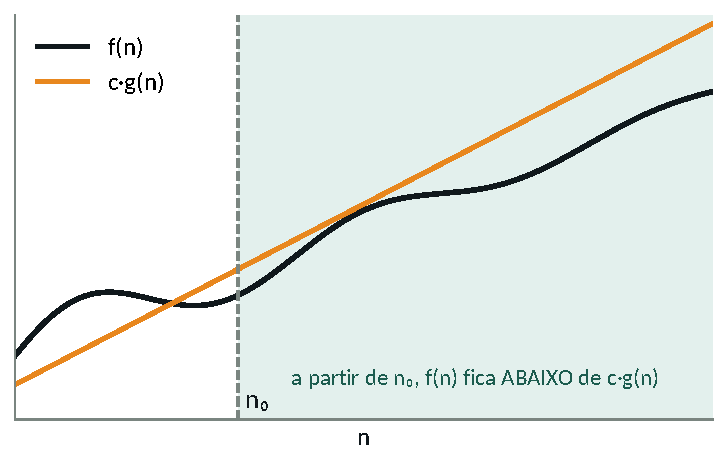
\includegraphics[width=0.72\textwidth]{figuras/f05_definicao_O.pdf}
  \caption{Antes de $n_0$, $f$ pode até passar do teto. Na região destacada, nunca mais.}
\end{figure}

\section{Exemplo guiado: \texorpdfstring{$3n + 4 = O(n)$}{3n + 4 = O(n)}}

Queremos mostrar que existe um par $(c, n_0)$ com $3n + 4 \le c \cdot n$ para todo $n \ge n_0$.

\begin{enumerate}
  \item \textbf{Escolha um $c$ um pouco maior que o coeficiente de $n$.} O coeficiente é 3;
        vamos tentar $c = 4$.
  \item \textbf{Resolva a desigualdade:} $3n + 4 \le 4n$ \ $\Longleftrightarrow$ \ $4 \le 4n - 3n$
        \ $\Longleftrightarrow$ \ $4 \le n$.
  \item \textbf{Leia o resultado:} a desigualdade vale para todo $n \ge 4$. Então $n_0 = 4$.
\end{enumerate}

Conferindo com números:

\begin{center}
\begin{tabularx}{0.9\textwidth}{L C C C C C C}
\cab \tcx{$n$} & \tc{1} & \tc{2} & \tc{3} & \tc{4} & \tc{5} & \tc{6} \\
$3n + 4$ & 7 & 10 & 13 & 16 & 19 & 22 \\
\rowcolor{edfundo} $4n$ & 4 & 8 & 12 & 16 & 20 & 24 \\
vale $3n + 4 \le 4n$? & não & não & não & \textbf{sim} & \textbf{sim} & \textbf{sim} \\
\end{tabularx}
\end{center}

\begin{figure}[!htb]
  \centering
  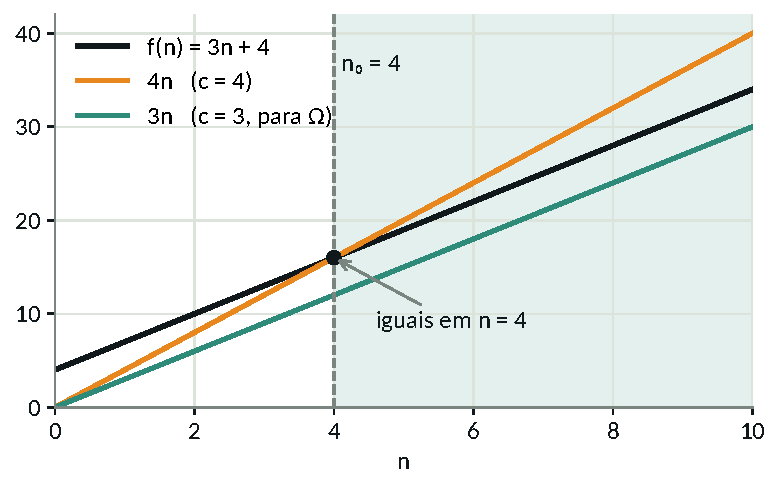
\includegraphics[width=0.7\textwidth]{figuras/f05_exemplo_3n4.pdf}
  \caption{$3n + 4$ fica abaixo de $4n$ a partir de $n_0 = 4$. (A reta $3n$ será usada no capítulo 6.)}\label{fig:exemplo3n4}
\end{figure}

Encontramos $c = 4$ e $n_0 = 4$; logo, $3n + 4 = O(n)$. Outros pares também servem: com $c = 7$,
por exemplo, a desigualdade $3n + 4 \le 7n$ vale desde $n_0 = 1$. A definição só pede que
\textbf{exista} um par.

\section{Uma técnica que sempre funciona para polinômios}

Para mostrar que $2n^2 + 3n + 1 = O(n^2)$: para $n \ge 1$, temos $n \le n^2$ e $1 \le n^2$.
Então podemos trocar cada termo pelo maior deles:
\[
2n^2 + 3n + 1 \;\le\; 2n^2 + 3n^2 + 1n^2 \;=\; 6n^2 \qquad \text{para todo } n \ge 1.
\]
Logo, $c = 6$ e $n_0 = 1$ funcionam. O truque: \textbf{some os coeficientes} e use o resultado
como $c$.

\section{Como mostrar que algo NÃO é \texorpdfstring{$O$}{O}}

Será que $n^2 = O(n)$? Se fosse, existiriam $c$ e $n_0$ com $n^2 \le c \cdot n$ para todo
$n \ge n_0$. Dividindo os dois lados por $n$ (que é positivo), isso vira $n \le c$. Mas $n$ cresce
sem parar e $c$ é fixo: basta tomar $n = c + 1$ (e maior que $n_0$) para a desigualdade falhar.
Nenhuma constante segura $n^2$ debaixo de $c \cdot n$. Portanto, $n^2$ \textbf{não} é $O(n)$.

\section{O é um teto — e pode ser folgado}

É verdade que $3n + 4 = O(n^2)$: um teto quadrático é alto o suficiente para uma função linear.
Mas essa informação é pobre, como dizer que \enquote{um carro custa menos que um bilhão de reais}.
Na prática, sempre buscamos o teto \textbf{mais justo} possível: $3n + 4 = O(n)$. Quando quisermos
dizer que o teto é exato, usaremos a notação $\Theta$ (capítulo 7).

\begin{atencao}
Três erros comuns:
\begin{itemize}
  \item Escrever $O(2n)$ ou $O(n^2 + n)$: as constantes e os termos menores devem ser removidos.
        Escreva $O(n)$ e $O(n^2)$.
  \item Achar que $O(n)$ quer dizer \enquote{exatamente $n$ passos}. Quer dizer \enquote{no máximo
        proporcional a $n$, para $n$ grande}.
  \item Achar que $O$ significa \enquote{pior caso}. $O$ é uma forma de comparar funções; o pior
        caso é uma situação dos dados. Voltaremos a isso nos capítulos 8 e 9.
\end{itemize}
\end{atencao}

\begin{exrapido}
Mostre que $2n + 10 = O(n)$, encontrando um par $c$ e $n_0$.
\end{exrapido}

\begin{exrapido}
(a) $7 = O(1)$? Encontre $c$ e $n_0$. (b) $n^2 + 100 = O(n^2)$? (c) $n^2 = O(n)$?
\end{exrapido}

\begin{respostas}
  \resp{5.1} Com $c = 3$: $2n + 10 \le 3n \Longleftrightarrow 10 \le n$. Então $c = 3$ e $n_0 = 10$.
  Outra resposta válida: com $c = 12$, $2n + 10 \le 12n$ vale desde $n_0 = 1$ (pela técnica de
  somar os coeficientes).
  \resp{5.2} (a) Sim: $7 \le 7 \cdot 1$ sempre, com $c = 7$ e $n_0 = 1$. Custo constante é $O(1)$.
  (b) Sim: $n^2 + 100 \le n^2 + 100n^2 = 101n^2$ para $n \ge 1$ ($c = 101$, $n_0 = 1$); ou
  $n^2 + 100 \le 2n^2$ para $n \ge 10$ ($c = 2$, $n_0 = 10$). (c) Não: veja a seção 5.5.
\end{respostas}

% =====================================================================
\chapter{Notação Ω: o piso}\label{cap:06}
\naaula{24, 26 e 27}

Se $O$ é um teto, $\Omega$ (lê-se \enquote{ômega grande}) é um \textbf{piso}: escrever
$f(n) = \Omega(g(n))$ significa que \textbf{$f$ cresce pelo menos tão rápido quanto $g$}.

\section{A definição}

\begin{center}
\colorbox{edtealclaro}{\parbox{0.92\textwidth}{\centering\large
$f(n) = \Omega(g(n))$ \ se existem constantes $c > 0$ e $n_0 \ge 1$ tais que\\[0.3em]
$f(n) \ge c \cdot g(n)$ \ para todo $n \ge n_0$.}}
\end{center}

É a mesma definição do $O$, com a desigualdade virada: agora $f$ fica \textbf{acima} de
$c \cdot g$ a partir de $n_0$.

\begin{figure}[!htb]
  \centering
  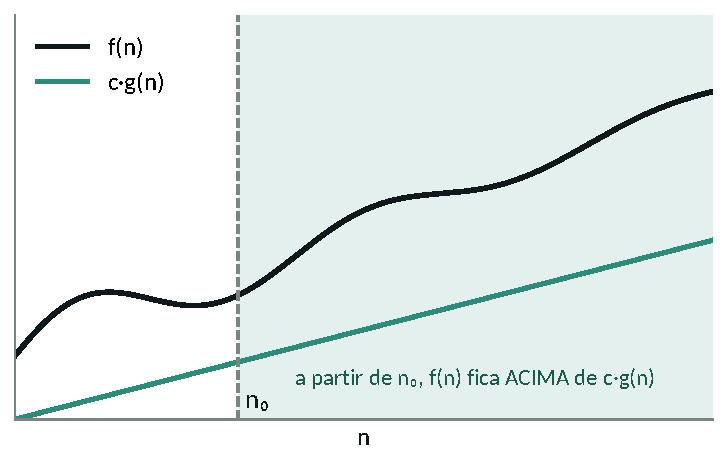
\includegraphics[width=0.72\textwidth]{figuras/f06_definicao_Omega.pdf}
  \caption{A partir de $n_0$, $f$ nunca desce abaixo do piso $c \cdot g(n)$.}
\end{figure}

\section{Exemplos}

\textbf{$3n + 4 = \Omega(n)$.} Com $c = 3$: $3n + 4 \ge 3n$ vale para todo $n \ge 1$ (o $+4$ só
ajuda). Então $c = 3$ e $n_0 = 1$. (É a reta $3n$ da figura~\ref{fig:exemplo3n4}.)

\textbf{$\dfrac{n^2}{2} - 3n = \Omega(n^2)$.} Aqui há um termo \emph{subtraindo}, então precisamos
de um pouco mais de cuidado. Vamos tentar $c = \dfrac{1}{4}$:
\[
\frac{n^2}{2} - 3n \ge \frac{n^2}{4}
\;\Longleftrightarrow\; \frac{n^2}{4} \ge 3n
\;\Longleftrightarrow\; n \ge 12.
\]
Então $c = \dfrac{1}{4}$ e $n_0 = 12$ funcionam. A ideia: \enquote{gastamos} metade do termo
dominante para cobrir o termo negativo, que é menor.

\section{Ω também descreve problemas}

A notação $\Omega$ tem um uso muito poderoso: dizer que um \textbf{problema} exige, no mínimo,
certo trabalho, qualquer que seja o algoritmo.

\begin{intuicao}
Achar o maior valor de uma lista \textbf{não ordenada} com $n$ elementos exige olhar todos os
$n$. Por quê? Se algum algoritmo deixasse de olhar um único elemento, esse elemento poderia ser
justamente o maior, e o algoritmo erraria. Então todo algoritmo correto para esse problema faz
pelo menos $n$ leituras: o problema é $\Omega(n)$. Nenhuma ideia genial, em nenhuma linguagem,
consegue fazer melhor.
\end{intuicao}

\section{Como mostrar que algo NÃO é Ω}

Será que $n = \Omega(n^2)$? Precisaríamos de $n \ge c \cdot n^2$, ou seja, $1 \ge c \cdot n$,
ou ainda $n \le \dfrac{1}{c}$. Como $n$ cresce sem parar, isso falha para $n$ grande. Então
$n$ \textbf{não} é $\Omega(n^2)$: uma função linear não cresce tão rápido quanto uma quadrática.

\begin{exrapido}
(a) Mostre que $5n - 20 = \Omega(n)$. (b) $n = \Omega(n^2)$? (c) $n^2 = \Omega(n)$?
\end{exrapido}

\begin{respostas}
  \resp{6.1} (a) Com $c = 1$: $5n - 20 \ge n \Longleftrightarrow 4n \ge 20 \Longleftrightarrow n \ge 5$.
  Então $c = 1$ e $n_0 = 5$. (b) Não (seção 6.4). (c) Sim: $n^2 \ge 1 \cdot n$ para todo $n \ge 1$.
  Um piso baixo é sempre verdadeiro, mas, como o teto alto do $O$, é pouco informativo.
\end{respostas}

% =====================================================================
\chapter{Notação Θ: o crescimento exato}\label{cap:07}
\naaula{25 a 27}

Quando uma função tem o mesmo $g$ como teto \emph{e} como piso, sabemos exatamente como ela
cresce. É isso que a notação $\Theta$ (lê-se \enquote{teta grande}) expressa.

\section{A definição}

\begin{center}
\colorbox{edtealclaro}{\parbox{0.92\textwidth}{\centering\large
$f(n) = \Theta(g(n))$ \ se existem constantes $c_1 > 0$, $c_2 > 0$ e $n_0 \ge 1$ tais que\\[0.3em]
$c_1 \cdot g(n) \;\le\; f(n) \;\le\; c_2 \cdot g(n)$ \ para todo $n \ge n_0$.}}
\end{center}

Em outras palavras: $f(n) = \Theta(g(n))$ quando $f(n) = O(g(n))$ \textbf{e} $f(n) = \Omega(g(n))$.
A função fica \enquote{ensanduichada} entre dois múltiplos de $g$.

\begin{figure}[!htb]
  \centering
  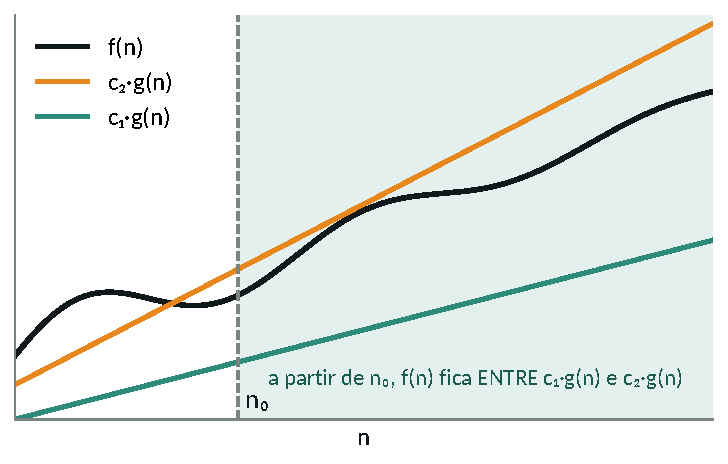
\includegraphics[width=0.72\textwidth]{figuras/f07_definicao_Theta.pdf}
  \caption{A partir de $n_0$, $f$ fica presa na faixa entre $c_1 \cdot g(n)$ e $c_2 \cdot g(n)$.}
\end{figure}

\section{Exemplos}

\textbf{$3n + 4 = \Theta(n)$.} Já temos as duas metades: no capítulo 5, $3n + 4 \le 4n$ para
$n \ge 4$; no capítulo 6, $3n + 4 \ge 3n$ para $n \ge 1$. Juntando, com $c_1 = 3$, $c_2 = 4$ e
$n_0 = 4$ (o maior dos dois $n_0$):
\[
3n \;\le\; 3n + 4 \;\le\; 4n \qquad \text{para todo } n \ge 4.
\]

\textbf{$n^2 + n = \Theta(n^2)$.} Para $n \ge 1$: $n^2 \le n^2 + n$ (óbvio) e
$n^2 + n \le n^2 + n^2 = 2n^2$. Então $c_1 = 1$, $c_2 = 2$ e $n_0 = 1$.

\section{Resumo das três notações}

\begin{center}
\begin{tabularx}{\textwidth}{P{1.6cm} P{2.6cm} P{2.6cm} P{3.3cm} L}
\cab \tc{Notação} & \tc{Lê-se} & \tc{Ideia} & \tc{Desigualdade} & \tc{Como comparar números} \\
$O(g)$ & ó grande & teto & $f \le c \cdot g$ & como \enquote{$\le$} \\
\rowcolor{edfundo} $\Omega(g)$ & ômega grande & piso & $f \ge c \cdot g$ & como \enquote{$\ge$} \\
$\Theta(g)$ & teta grande & crescimento exato & $c_1 g \le f \le c_2 g$ & como \enquote{$=$} \\
\end{tabularx}
\end{center}

\begin{intuicao}
A comparação com números ajuda a lembrar: dizer $f = O(g)$ é como dizer \enquote{a velocidade de
crescimento de $f$ é $\le$ a de $g$}; $\Omega$ é \enquote{$\ge$}; e $\Theta$ é \enquote{$=$}.
Sempre em termos de \emph{forma de crescimento}, ignorando constantes.
\end{intuicao}

\section{Uma regra prática para polinômios}

Se $f(n)$ é um polinômio cujo maior expoente é $d$ e o coeficiente desse termo é positivo, então
$f(n) = \Theta(n^d)$. Exemplos: $3n + 4 = \Theta(n)$; $3n^2 + 4n + 2 = \Theta(n^2)$;
$\dfrac{n(n-1)}{2} = \Theta(n^2)$. É a formalização exata da ideia de termo dominante do
capítulo 4.

\begin{conexao}
Agora dá para dizer com precisão alguns custos das aulas anteriores:
\begin{itemize}
  \item \codigo{empilhar()}, \codigo{desempilhar()} e \codigo{consultar_topo()} da Pilha: $\Theta(1)$.
  \item \codigo{enfileirar()} e \codigo{desenfileirar()} da Fila com ponteiro para o fim: $\Theta(1)$.
  \item \codigo{percorrer()} de qualquer Lista com $n$ elementos: $\Theta(n)$.
  \item Inserir $n$ elementos, um a um, no início de uma lista contígua: $\dfrac{n(n-1)}{2}$
        deslocamentos, ou seja, $\Theta(n^2)$.
\end{itemize}
\end{conexao}

\begin{exrapido}
(a) Mostre que $3n + 4 = \Theta(n)$, dando $c_1$, $c_2$ e $n_0$. (b) Mostre que
$4n^2 - 10n + 7 = \Theta(n^2)$. (Dica para o piso: $7 \ge 0$ e \enquote{gaste} metade do $4n^2$
com o $-10n$.)
\end{exrapido}

\begin{respostas}
  \resp{7.1} (a) $c_1 = 3$, $c_2 = 4$, $n_0 = 4$ (seção 7.2).
  (b) \emph{Teto:} para $n \ge 1$, $-10n \le 0$ e $7 \le 7n^2$, então $4n^2 - 10n + 7 \le 4n^2 + 7n^2 = 11n^2$.
  \emph{Piso:} como $7 \ge 0$, temos $4n^2 - 10n + 7 \ge 4n^2 - 10n$, e
  $4n^2 - 10n \ge 2n^2 \Longleftrightarrow 2n^2 \ge 10n \Longleftrightarrow n \ge 5$.
  Logo, $c_1 = 2$, $c_2 = 11$ e $n_0 = 5$.
\end{respostas}

% =====================================================================
\chapter{Melhor, pior e caso médio}\label{cap:08}
\naaula{28}

No capítulo 2, a busca linear custou 4 passos quando o valor estava na primeira posição e $3n + 3$
quando não estava na lista. O mesmo algoritmo, com o mesmo $n$, tem custos muito diferentes:
tudo depende dos \textbf{dados}. Este capítulo organiza essa ideia.

\section{Três perguntas diferentes}

Para uma entrada de tamanho $n$, podemos perguntar:

\begin{itemize}
  \item \textbf{Melhor caso:} qual é o \emph{menor} custo possível, escolhendo os dados mais
        favoráveis?
  \item \textbf{Pior caso:} qual é o \emph{maior} custo possível, com os dados mais desfavoráveis?
  \item \textbf{Caso médio:} qual é o custo \emph{esperado}, em média, para dados típicos?
\end{itemize}

Cada resposta é uma função de $n$ diferente. Vamos calculá-las para a busca linear, contando só
as comparações \codigo{dados[i] == valor}.

\begin{figure}[!htb]
\centering
\begin{tikzpicture}[scale=0.62, every node/.style={font=\small}]
  \foreach \lin/\nome/\alvo/\cor in {0/melhor caso/1/edteal, 1/caso médio/5/edlaranja, 2/pior caso/9/edverde} {
    \node[anchor=east, font=\small\bfseries] at (-0.4, -\lin*1.8+0.5) {\nome};
    \foreach \i in {1,...,9} {
      \pgfmathsetmacro{\preench}{\i <= \alvo ? 1 : 0}
      \ifdim\preench pt=1pt
        \draw[fill=\cor!25, draw=\cor, line width=0.8pt] (\i-1, -\lin*1.8) rectangle ++(1,1);
      \else
        \draw[fill=white, draw=edcinzaclaro, line width=0.8pt] (\i-1, -\lin*1.8) rectangle ++(1,1);
      \fi
    }
    \draw[-{Latex}, line width=1pt, \cor] (\alvo-0.5, -\lin*1.8+1.7) -- (\alvo-0.5, -\lin*1.8+1.05);
  }
  \node[anchor=west] at (9.4, 0.5) {1 comparação};
  \node[anchor=west] at (9.4, -1.3) {em média, $(n+1)/2$};
  \node[anchor=west] at (9.4, -3.1) {$n$ comparações};
\end{tikzpicture}
\caption{Busca linear num vetor de 9 posições: as células coloridas são as comparadas até achar o
valor (seta).}
\end{figure}

\section{A busca linear, caso a caso}

\textbf{Melhor caso:} o valor está na posição 0. Uma comparação e pronto: custo $\Theta(1)$.

\textbf{Pior caso:} o valor está na última posição ou não está na lista. São $n$ comparações:
custo $\Theta(n)$.

\textbf{Caso médio:} suponha que o valor está na lista e que qualquer posição é igualmente
provável. Se ele está na posição 1, fazemos 1 comparação; na posição 2, fazemos 2; \dots; na
posição $n$, fazemos $n$. A média é a soma dividida por $n$ — e a soma é a de Gauss:
\[
\text{média} \;=\; \frac{1 + 2 + \dots + n}{n} \;=\; \frac{n(n+1)/2}{n} \;=\; \frac{n+1}{2}.
\]
Em média, olhamos cerca de metade da lista. Mas \enquote{metade de $n$} ainda cresce como $n$:
o caso médio também é $\Theta(n)$.

\begin{center}
\begin{tabularx}{\textwidth}{L C C L}
\cab \tc{Caso} & \tc{Comparações} & \tc{Crescimento} & \tc{Quando acontece} \\
Melhor & 1 & $\Theta(1)$ & valor na primeira posição \\
\rowcolor{edfundo} Médio & $\dfrac{n+1}{2}$ & $\Theta(n)$ & valor numa posição qualquer \\
Pior & $n$ & $\Theta(n)$ & valor no fim ou ausente \\
\end{tabularx}
\end{center}

\section{Qual caso importa mais?}

\begin{itemize}
  \item O \textbf{pior caso} é uma \emph{garantia}: o algoritmo nunca será mais lento que isso.
        É o mais usado, principalmente em sistemas em que atrasar não é aceitável.
  \item O \textbf{caso médio} descreve o desempenho típico, mas exige supor como os dados
        costumam ser — e nem sempre sabemos.
  \item O \textbf{melhor caso} raramente serve para escolher um algoritmo (é fácil ter sorte), mas
        mostra o mínimo que o algoritmo faz e, às vezes, revela situações práticas importantes,
        como dados quase ordenados (capítulo 9).
\end{itemize}

\section{Mais dois exemplos das aulas anteriores}

\textbf{O \codigo{conjunto_inserir()} da Aula 3} chama \codigo{pertence()} antes de inserir, para
não duplicar. Num Conjunto com $n$ elementos:
\begin{itemize}
  \item melhor caso: o valor já é o primeiro elemento; \codigo{pertence()} acha na primeira
        comparação e a inserção é recusada: $\Theta(1)$;
  \item pior caso: o valor é novo; \codigo{pertence()} compara com todos os $n$ e depois
        insere no fim: $\Theta(n)$.
\end{itemize}
E se inserirmos $n$ valores \emph{distintos}, um a um, num Conjunto vazio? A primeira inserção
compara com 0 elementos, a segunda com 1, \dots, a última com $n - 1$: de novo a soma de Gauss,
$\dfrac{n(n-1)}{2}$ comparações, ou seja, $\Theta(n^2)$. É por isso que o \codigo{set()} do
Python usa outra estrutura (as tabelas de dispersão, assunto de um curso mais adiante).

\textbf{A função \codigo{maior()} do exercício 2.1} fez $3n + 1$ passos no melhor caso e $4n$ no
pior. Os números mudam, mas os dois casos são $\Theta(n)$. Nem sempre o caso muda a
\emph{família} do crescimento — mas, às vezes, muda, como você verá no capítulo 9.

\section{Casos e notações não são a mesma coisa}

\begin{atencao}
É muito comum confundir \enquote{$O$ = pior caso} e \enquote{$\Omega$ = melhor caso}. Não é isso!
\begin{itemize}
  \item \textbf{Melhor, pior e médio} são \emph{situações dos dados}. Cada uma gera uma função de $n$.
  \item \textbf{$O$, $\Omega$ e $\Theta$} são \emph{formas de descrever o crescimento de uma função}.
\end{itemize}
Por isso podemos dizer, por exemplo, \enquote{o pior caso da busca linear é $\Theta(n)$} e
\enquote{o melhor caso é $\Theta(1)$}. O capítulo 9 mostra essa distinção com o Insertion Sort,
em que o melhor e o pior caso pertencem a famílias diferentes.
\end{atencao}

\begin{exrapido}[18]
Considere a função abaixo, que verifica se uma lista tem algum valor repetido.
(a) Qual é o melhor caso e quantas comparações ele faz? (b) Qual é o pior caso e quantas
comparações ele faz? (c) Escreva os dois com a notação $\Theta$.

\begin{lstlisting}
def tem_repetido(v):
    for i in range(len(v)):
        for j in range(i + 1, len(v)):
            if v[i] == v[j]:
                return True
    return False
\end{lstlisting}
\end{exrapido}

\begin{exrapido}
Numa busca linear num vetor de 9 elementos, com o valor presente e todas as posições igualmente
prováveis, quantas comparações são feitas em média?
\end{exrapido}

\begin{respostas}
  \resp{8.1} (a) Melhor caso: \codigo{v[0] == v[1]}. A primeira comparação já encontra a
  repetição: 1 comparação. (b) Pior caso: não há nenhum valor repetido, e todas as duplas são
  comparadas. Para \codigo{i = 0}, são $n - 1$ comparações; para \codigo{i = 1}, $n - 2$; \dots;
  no total, $(n-1) + (n-2) + \dots + 1 + 0 = \dfrac{n(n-1)}{2}$. (c) Melhor caso $\Theta(1)$;
  pior caso $\Theta(n^2)$.
  \resp{8.2} $\dfrac{9 + 1}{2} = 5$ comparações.
\end{respostas}

\IfFileExists{capitulos/cap09.tex}{% =====================================================================
\chapter{Estudo de caso: Insertion Sort}\label{cap:09}
\naaula{29 a 36}

Este capítulo junta tudo o que vimos: contagem de operações, somatórios, as notações e os casos.
O personagem é um algoritmo de ordenação simples e muito usado na prática, o \textbf{Insertion
Sort} (ordenação por inserção), cujo custo depende fortemente de como os dados chegam.

\section{A ideia: arrumar cartas na mão}

Pense em como você arruma cartas de baralho recebidas uma a uma: a parte da mão que você já
arrumou fica em ordem; quando chega uma carta nova, você a compara com as da direita para a
esquerda, abre espaço e a encaixa no lugar certo. O Insertion Sort faz exatamente isso num vetor:

\begin{enumerate}
  \item A parte da esquerda do vetor (no começo, só o primeiro elemento) já está ordenada.
  \item Pegamos o próximo elemento — a \textbf{chave}.
  \item Deslocamos para a direita todos os elementos ordenados maiores que a chave.
  \item Colocamos a chave no espaço que sobrou.
\end{enumerate}

\begin{conexao}
Os passos 3 e 4 são o \codigo{inserir(pos, valor)} da lista contígua da Aula 1: para inserir no
meio, é preciso deslocar os elementos seguintes. O Insertion Sort é uma sequência de
\enquote{inserções no lugar certo}, e o custo dele vem justamente desses deslocamentos.
\end{conexao}

\section{O código}

\begin{lstlisting}
def insertion_sort(v):
    for i in range(1, len(v)):
        chave = v[i]
        j = i - 1
        while j >= 0 and v[j] > chave:
            v[j + 1] = v[j]      # desloca para a direita
            j -= 1
        v[j + 1] = chave         # encaixa a chave
\end{lstlisting}

\begin{lstlisting}[style=c]
void insertion_sort(int v[], int n) {
    for (int i = 1; i < n; i++) {
        int chave = v[i];
        int j = i - 1;
        while (j >= 0 && v[j] > chave) {
            v[j + 1] = v[j];     /* desloca para a direita */
            j--;
        }
        v[j + 1] = chave;        /* encaixa a chave */
    }
}
\end{lstlisting}

Para analisar, vamos contar duas coisas: as \textbf{comparações} (cada avaliação de
\codigo{v[j] > chave}) e os \textbf{deslocamentos} (cada \codigo{v[j + 1] = v[j]}).

\section{Passo a passo}

\begin{figure}[!htb]
\centering
\begin{tikzpicture}[scale=0.62]
  \linhaIns{0}{5,2,4,6,1,3}{1}{0}{início: a parte ordenada é só o 5}
  \linhaIns{-1.3}{2,5,4,6,1,3}{2}{1}{passada 1, chave 2: 1 comparação, 1 deslocamento}
  \linhaIns{-2.6}{2,4,5,6,1,3}{3}{2}{passada 2, chave 4: 2 comparações, 1 deslocamento}
  \linhaIns{-3.9}{2,4,5,6,1,3}{4}{4}{passada 3, chave 6: 1 comparação, 0 deslocamentos}
  \linhaIns{-5.2}{1,2,4,5,6,3}{5}{1}{passada 4, chave 1: 4 comparações, 4 deslocamentos}
  \linhaIns{-6.5}{1,2,3,4,5,6}{6}{3}{passada 5, chave 3: 4 comparações, 3 deslocamentos}
\end{tikzpicture}
\caption{Ordenando $[5, 2, 4, 6, 1, 3]$. Em verde, a parte ordenada; em laranja, onde a chave foi
encaixada. Total: 12 comparações e 9 deslocamentos.}
\end{figure}

Repare na passada 4: a chave 1 é menor que todos os ordenados, então é comparada com os quatro,
todos se deslocam, e o laço para porque \codigo{j} chega a $-1$ (sem uma quinta comparação). Na
passada 3, a chave 6 já é maior que o último ordenado: uma comparação, nenhum deslocamento.

\section{Melhor caso: o vetor já está ordenado}

\begin{figure}[!htb]
\centering
\begin{minipage}{0.48\textwidth}\centering
\begin{tikzpicture}[scale=0.5]
  \linhaIns{0}{1,2,3,4,5}{1}{0}{}
  \linhaIns{-1.3}{1,2,3,4,5}{2}{2}{}
  \linhaIns{-2.6}{1,2,3,4,5}{3}{3}{}
  \linhaIns{-3.9}{1,2,3,4,5}{4}{4}{}
  \linhaIns{-5.2}{1,2,3,4,5}{5}{5}{}
  \foreach \k in {1,...,4} \node[anchor=west, font=\footnotesize] at (5.2, -\k*1.3+0.45) {1 comp., 0 desl.};
\end{tikzpicture}
\par\small\textbf{Melhor caso:} $[1, 2, 3, 4, 5]$
\end{minipage}\hfill
\begin{minipage}{0.48\textwidth}\centering
\begin{tikzpicture}[scale=0.5]
  \linhaIns{0}{5,4,3,2,1}{1}{0}{}
  \linhaIns{-1.3}{4,5,3,2,1}{2}{1}{}
  \linhaIns{-2.6}{3,4,5,2,1}{3}{1}{}
  \linhaIns{-3.9}{2,3,4,5,1}{4}{1}{}
  \linhaIns{-5.2}{1,2,3,4,5}{5}{1}{}
  \foreach \k in {1,...,4} \node[anchor=west, font=\footnotesize] at (5.2, -\k*1.3+0.45) {\k\ comp., \k\ desl.};
\end{tikzpicture}
\par\small\textbf{Pior caso:} $[5, 4, 3, 2, 1]$
\end{minipage}
\caption{À esquerda, cada chave já está no lugar: uma comparação por passada. À direita, cada
chave precisa ir até o início: as passadas custam 1, 2, 3 e 4.}
\end{figure}

Se o vetor já está em ordem crescente, cada chave é comparada só com o elemento à sua esquerda,
descobre que já está no lugar e nenhum deslocamento acontece. São $n - 1$ passadas com 1
comparação cada:
\[
T_{\text{melhor}}(n) = n - 1 \text{ comparações} \qquad\Longrightarrow\qquad T_{\text{melhor}}(n) = \Theta(n).
\]

\section{Pior caso: ordem inversa}

Se o vetor está em ordem decrescente, cada chave é menor que todos os já ordenados: na passada
$i$, ela é comparada com os $i$ elementos da esquerda e todos se deslocam. Somando as passadas —
a soma de Gauss do capítulo 3:
\[
T_{\text{pior}}(n) = 1 + 2 + \dots + (n-1) = \frac{n(n-1)}{2} \text{ comparações}
\qquad\Longrightarrow\qquad T_{\text{pior}}(n) = \Theta(n^2).
\]
Para $n = 1.000$, são 499.500 comparações — contra 999 do melhor caso.

\section{Caso médio: ordem aleatória}

Com os dados embaralhados, cada chave, em média, é maior que metade dos elementos já ordenados e
menor que a outra metade. Então ela anda, em média, metade do caminho: na passada $i$, cerca de
$i/2$ comparações. Somando, chegamos à metade do pior caso:
\[
T_{\text{médio}}(n) \approx \frac{1}{2} \cdot \frac{n(n-1)}{2} \approx \frac{n^2}{4}
\qquad\Longrightarrow\qquad T_{\text{médio}}(n) = \Theta(n^2).
\]

\begin{center}
\begin{tabularx}{0.95\textwidth}{C C C C C}
\cab \tcx{$n$} & \tc{Ordenado} & \tc{Aleatório (medido)} & \tc{Invertido} & \tcx{$n^2/4$} \\
10 & 9 & 30 & 45 & 25 \\
\rowcolor{edfundo} 100 & 99 & 2.607 & 4.950 & 2.500 \\
1.000 & 999 & 252.249 & 499.500 & 250.000 \\

\end{tabularx}
\end{center}

\begin{figure}[!htb]
  \centering
  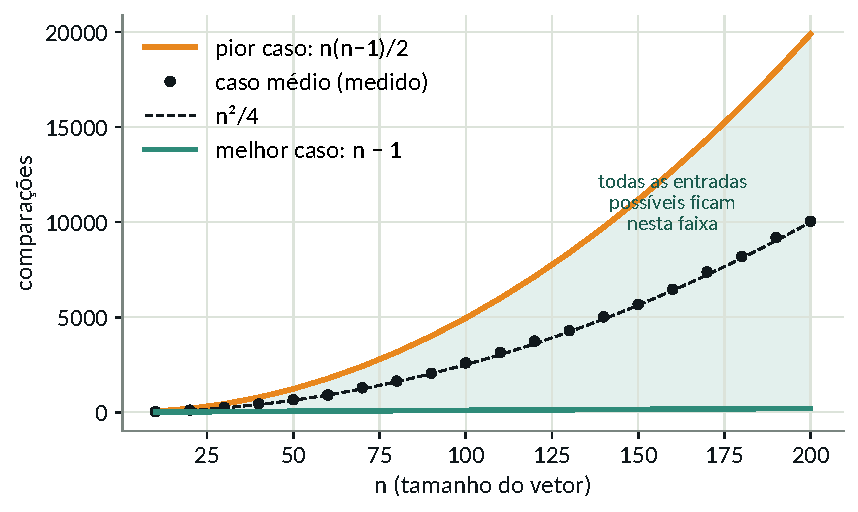
\includegraphics[width=0.74\textwidth]{figuras/f09_insertion_casos.pdf}
  \caption{Comparações do Insertion Sort nos três cenários. O caso médio (pontos) acompanha
  $n^2/4$, e o melhor caso quase não sai do chão.}
\end{figure}

\begin{atencao}
Metade do pior caso continua sendo quadrático! Dividir por 2 é multiplicar por uma constante, e
constantes não mudam a família. Em média, o Insertion Sort é tão \enquote{quadrático} quanto no pior
caso — só com a metade do trabalho.
\end{atencao}

\section{Vendo na prática}

O programa \codigo{python/insertion_sort.py} (e a versão em C) faz o passo a passo e conta as
comparações nos três cenários. Esta é a saída real:

\needspace{22\baselineskip}
\lstinputlisting[style=terminal]{tabelas/saida_insertion.txt}

Os números do caso aleatório mudam um pouco entre o Python e o C, porque os dois usam geradores
de números aleatórios diferentes. Mas ambos ficam perto de $n^2/4$.

\section{Onde entram \texorpdfstring{$O$, $\Omega$ e $\Theta$}{O, Ω e Θ}}

Este é o ponto que mais confunde — e o Insertion Sort é o exemplo perfeito para esclarecê-lo.

\begin{itemize}
  \item Cada \textbf{caso} é uma função diferente: $T_{\text{melhor}}(n) = n - 1$ e
        $T_{\text{pior}}(n) = \dfrac{n(n-1)}{2}$.
  \item Cada função pode ser descrita com a notação $\Theta$:
        $T_{\text{melhor}}(n) = \Theta(n)$ e $T_{\text{pior}}(n) = \Theta(n^2)$.
  \item Para \textbf{qualquer} entrada, o custo fica na faixa entre essas duas curvas (a região
        destacada na figura acima). Então podemos dizer: o custo do Insertion Sort é
        $O(n^2)$ (nunca passa do pior caso) e $\Omega(n)$ (nunca fica abaixo do melhor caso).
\end{itemize}

\begin{atencao}
Não diga \enquote{o Insertion Sort é $\Theta(n^2)$} sem dizer de qual caso está falando: no melhor
caso ele é $\Theta(n)$! Frases corretas: \enquote{o pior caso do Insertion Sort é $\Theta(n^2)$};
\enquote{o Insertion Sort é $O(n^2)$}; \enquote{o melhor caso é $\Theta(n)$}. E lembre: $O$ não é
sinônimo de pior caso, nem $\Omega$ de melhor caso — são as notações que usamos para descrever
cada caso.
\end{atencao}

\section{Dados quase ordenados}

O melhor caso não é só uma curiosidade. Muitos dados reais chegam \emph{quase} ordenados: uma
lista de chamada com um aluno novo no fim, um histórico em que só o último registro está fora do
lugar. Nesses casos, o Insertion Sort faz pouco mais que $n$ comparações.

\begin{aprofunde}
Chamamos de \textbf{inversão} cada par de elementos fora de ordem (um maior antes de um menor).
Cada deslocamento do Insertion Sort desfaz exatamente uma inversão; por isso o número de
deslocamentos é igual ao número de inversões do vetor. Um vetor ordenado tem 0 inversões; um
invertido tem o máximo, $\dfrac{n(n-1)}{2}$; um embaralhado tem, em média, $\dfrac{n(n-1)}{4}$.
Por isso o \codigo{sort()} do Python (um algoritmo chamado Timsort) usa o Insertion Sort em
trechos pequenos: nesses trechos, ele é o mais rápido.
\end{aprofunde}

\begin{exrapido}
Aplique o Insertion Sort a $[1, 2, 3, 5, 4]$. Quantas comparações e quantos deslocamentos são
feitos? O resultado está mais perto do melhor ou do pior caso?
\end{exrapido}

\begin{exrapido}
(a) Para $n = 8$, quantas comparações o Insertion Sort faz no melhor caso? E no pior?
(b) Quantos deslocamentos são feitos para ordenar $[4, 3, 2, 1]$?
\end{exrapido}

\begin{respostas}
  \resp{9.1} Passadas 1, 2 e 3 (chaves 2, 3 e 5): 1 comparação cada, nenhum deslocamento.
  Passada 4 (chave 4): compara com 5 (desloca) e com 3 (para): 2 comparações e 1 deslocamento.
  Total: 5 comparações e 1 deslocamento — quase o melhor caso ($n - 1 = 4$). O vetor tinha uma
  única inversão (o par 5, 4).
  \resp{9.2} (a) Melhor caso: $8 - 1 = 7$; pior caso: $\dfrac{8 \cdot 7}{2} = 28$.
  (b) $1 + 2 + 3 = 6$ deslocamentos (é o pior caso para $n = 4$).
\end{respostas}
}{}
\IfFileExists{capitulos/cap10.tex}{% =====================================================================
\chapter{Comparando famílias de funções}\label{cap:10}
\naaula{37 a 40}

Até aqui, encontramos custos constantes, logarítmicos, lineares, quadráticos, exponenciais e
fatoriais. Este capítulo coloca todos lado a lado e mostra, com números, por que a
\textbf{família} de uma função importa mais do que qualquer constante ou qualquer computador.

\section{A hierarquia}

\begin{center}
\colorbox{edtealclaro}{\large\quad $1 \;<\; \log n \;<\; \sqrt{n} \;<\; n \;<\; n \log n \;<\; n^2 \;<\; n^3 \;<\; 2^n \;<\; n!$\quad}
\end{center}

Leia \enquote{$<$} como \enquote{cresce mais devagar que}, para $n$ grande. Cada família tem
representantes que você já conhece:

\begin{center}
\begin{tabularx}{\textwidth}{P{2.4cm} P{2.8cm} L}
\cab \tc{Família} & \tc{Nome} & \tc{Exemplo} \\
$1$ & constante & \codigo{consultar_topo()}, \codigo{obter(pos)} na lista contígua \\
\rowcolor{edfundo} $\log n$ & logarítmica & adivinhar um número dividindo ao meio; busca binária \\
$\sqrt{n}$ & raiz & busca por saltos em vetor ordenado (capítulo 11) \\
\rowcolor{edfundo} $n$ & linear & \codigo{buscar()}, \codigo{percorrer()}, achar o maior valor \\
$n \log n$ & \enquote{n log n} & os melhores algoritmos de ordenação, como o \codigo{sort()} do Python \\
\rowcolor{edfundo} $n^2$ & quadrática & Insertion Sort no pior caso, interseção ingênua de conjuntos \\
$n^3$ & cúbica & três laços aninhados até $n$ \\
\rowcolor{edfundo} $2^n$ & exponencial & testar todos os subconjuntos de um Conjunto \\
$n!$ & fatorial & testar todas as ordens possíveis de uma fila \\
\end{tabularx}
\end{center}

\section{Os números}

A tabela abaixo foi gerada pelo programa \codigo{python/crescimento_funcoes.py}. Números enormes
aparecem em notação científica: $1{,}3 \times 10^{30}$ quer dizer 1,3 seguido de 30 casas.

\begin{center}
\begin{tabularx}{\textwidth}{P{2.1cm} C C C C C}
\cab \tc{Função} & \tcx{$n = 10$} & \tcx{$n = 20$} & \tcx{$n = 50$} & \tcx{$n = 100$} & \tcx{$n = 1.000$} \\
$\log_2 n$ & 3,3 & 4,3 & 5,6 & 6,6 & 10,0 \\
\rowcolor{edfundo} $\sqrt{n}$ & 3,2 & 4,5 & 7,1 & 10,0 & 31,6 \\
$n$ & 10 & 20 & 50 & 100 & 1.000 \\
\rowcolor{edfundo} $n \log_2 n$ & 33,2 & 86,4 & 282,2 & 664,4 & 9.966 \\
$n^2$ & 100 & 400 & 2.500 & 10.000 & 1.000.000 \\
\rowcolor{edfundo} $n^3$ & 1.000 & 8.000 & 125.000 & 1.000.000 & $1{,}0 \times 10^{9}$ \\
$2^n$ & 1.024 & 1.048.576 & $1{,}1 \times 10^{15}$ & $1{,}3 \times 10^{30}$ & $1{,}1 \times 10^{301}$ \\
\rowcolor{edfundo} $n!$ & 3.628.800 & $2{,}4 \times 10^{18}$ & $3{,}0 \times 10^{64}$ & $9{,}3 \times 10^{157}$ & $4{,}0 \times 10^{2567}$ \\

\end{tabularx}
\end{center}

\begin{intuicao}
Um número como $4{,}0 \times 10^{2567}$ (o valor de $1.000!$) não tem comparação com nada no
mundo real: estima-se que o universo inteiro tenha cerca de $10^{80}$ átomos.
\end{intuicao}

\section{Lendo um gráfico em escala logarítmica}

Se desenharmos essas funções num gráfico comum, $n!$ e $2^n$ disparam para fora da página e as
outras parecem grudadas no chão. A solução é a \textbf{escala logarítmica} no eixo vertical: cada
marca vale 10 vezes (ou mais) a anterior. Assim, números muito diferentes cabem no mesmo desenho.

\begin{figure}[!htb]
  \centering
  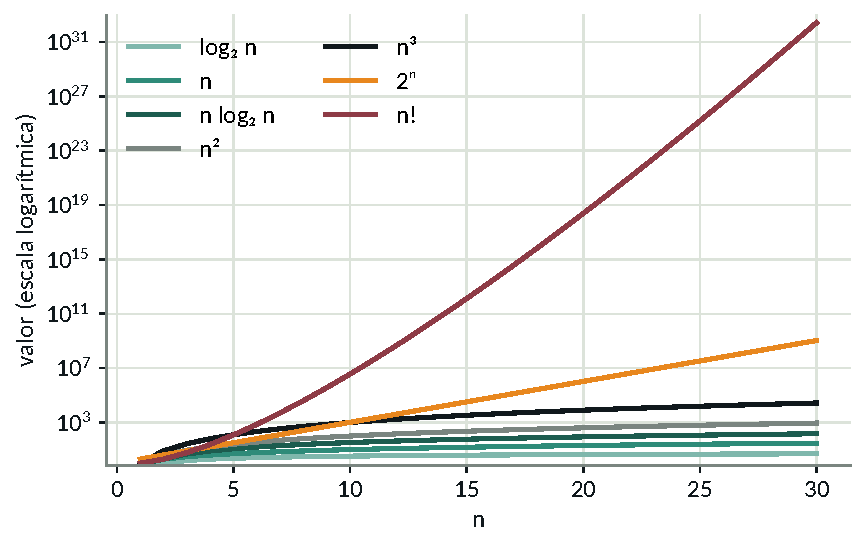
\includegraphics[width=0.76\textwidth]{figuras/f10_familias_log.pdf}
  \caption{As famílias em escala logarítmica. Cada marca do eixo vertical é $10^4$ vezes a
  anterior. $n!$ e $2^n$ se afastam de todas as outras.}
\end{figure}

\begin{atencao}
Numa escala logarítmica, curvas que parecem próximas podem estar muito distantes. A distância
vertical entre duas marcas vizinhas, aqui, é uma multiplicação por 10.000.
\end{atencao}

\section{Transformando em tempo}

Suponha um computador que execute um passo a cada nanossegundo (um bilionésimo de segundo),
ou seja, um bilhão de passos por segundo. Quanto tempo leva cada família?

\begin{center}
\begin{tabularx}{\textwidth}{P{2.1cm} C C C C}
\cab \tc{Passos} & \tcx{$n = 10$} & \tcx{$n = 20$} & \tcx{$n = 50$} & \tcx{$n = 100$} \\
$n$ & 10 ns & 20 ns & 50 ns & 100 ns \\
\rowcolor{edfundo} $n^2$ & 100 ns & 400 ns & 2,5 µs & 10,0 µs \\
$n^3$ & 1,0 µs & 8,0 µs & 125,0 µs & 1,0 ms \\
\rowcolor{edfundo} $2^n$ & 1,0 µs & 1,0 ms & 13 dias & $4{,}0 \times 10^{13}$ anos \\
$n!$ & 3,6 ms & 77 anos & $9{,}6 \times 10^{47}$ anos & $3{,}0 \times 10^{141}$ anos \\

\end{tabularx}
\end{center}
{\small ns = nanossegundo; µs = microssegundo (mil ns); ms = milissegundo (um milhão de ns).
Para comparar: a idade do universo é de cerca de $1{,}4 \times 10^{10}$ anos.}

Com $n = 100$, um algoritmo cúbico termina em 1 milissegundo; um exponencial levaria
$4 \times 10^{13}$ anos — milhares de vezes a idade do universo.

\section{E um computador mil vezes mais rápido?}

É tentador pensar que hardware melhor resolve tudo. Veja o maior $n$ que cabe em 1 segundo hoje
($10^9$ passos) e numa máquina 1.000 vezes mais rápida ($10^{12}$ passos):

\begin{center}
\begin{tabularx}{\textwidth}{P{2.1cm} C C L}
\cab \tc{Passos} & \tc{Maior n hoje} & \tc{Maior n, 1.000× mais rápido} & \tc{Ganho} \\
$n$ & $1{,}0 \times 10^{9}$ & $1{,}0 \times 10^{12}$ & 1.000 vezes maior \\
\rowcolor{edfundo} $n \log_2 n$ & $4{,}0 \times 10^{7}$ & $2{,}9 \times 10^{10}$ & 726 vezes maior \\
$n^2$ & 31.622 & 1.000.000 & 31{,}6 vezes maior \\
\rowcolor{edfundo} $n^3$ & 1.000 & 10.000 & 10{,}0 vezes maior \\
$2^n$ & 29 & 39 & só $+10$ \\
\rowcolor{edfundo} $n!$ & 12 & 14 & só $+2$ \\

\end{tabularx}
\end{center}

Para um algoritmo linear, a máquina nova resolve problemas 1.000 vezes maiores. Para um
quadrático, só 31,6 vezes maiores. Para um exponencial, o ganho é de \textbf{10 elementos}; para
um fatorial, de \textbf{2}. A moral:

\begin{center}
\colorbox{edlaranjaclaro}{\parbox{0.9\textwidth}{\centering\large
Trocar de computador multiplica a velocidade por uma constante.\\
Trocar de algoritmo pode mudar a família — e isso vale muito mais.}}
\end{center}

\begin{exrapido}
Ordene da que cresce mais devagar para a que cresce mais rápido:
$n^2$, $2^n$, $n \log n$, $100$, $n!$, $\sqrt{n}$, $n^3$, $\log n$.
\end{exrapido}

\begin{exrapido}
Um algoritmo exponencial ($2^n$ passos) leva 1 segundo para $n = 30$. (a) Quanto tempo leva para
$n = 31$? (b) E para $n = 40$? (c) Se o algoritmo fosse quadrático ($n^2$ passos) e levasse
1 segundo para $n = 30$, quanto levaria para $n = 40$?
\end{exrapido}

\begin{respostas}
  \resp{10.1} $100 < \log n < \sqrt{n} < n \log n < n^2 < n^3 < 2^n < n!$.
  \resp{10.2} (a) 2 segundos: cada $+1$ em $n$ dobra o tempo. (b) São 10 dobras:
  $2^{10} = 1.024$ segundos, cerca de 17 minutos. (c) O tempo cresce como $(40/30)^2 = 16/9$:
  cerca de 1,8 segundo.
\end{respostas}
}{}
\IfFileExists{capitulos/cap11.tex}{% =====================================================================
\chapter{Um toque de Cálculo}\label{cap:11}
\naaula{41 a 45}

Você não precisa ter estudado Cálculo para acompanhar este capítulo. Vamos usar uma única ideia —
a \textbf{derivada} — e uma única regra para calculá-la. Com elas, dá para medir quanto um custo
cresce a cada elemento a mais e até descobrir o melhor valor de um parâmetro de um algoritmo.

\section{Derivada: a inclinação de uma curva}

Nos capítulos anteriores, comparamos funções pelo \enquote{quanto crescem}. A derivada torna isso
preciso: ela mede \textbf{a taxa de crescimento} de uma função em cada ponto — quanto a saída
aumenta quando a entrada aumenta um pouquinho.

Graficamente, a derivada de $T$ no ponto $n$ é a \textbf{inclinação da reta tangente} (a reta que
só \enquote{encosta} na curva naquele ponto). Uma inclinação 4 quer dizer: perto daquele ponto,
cada unidade a mais em $n$ aumenta $T$ em cerca de 4.

\begin{figure}[!htb]
  \centering
  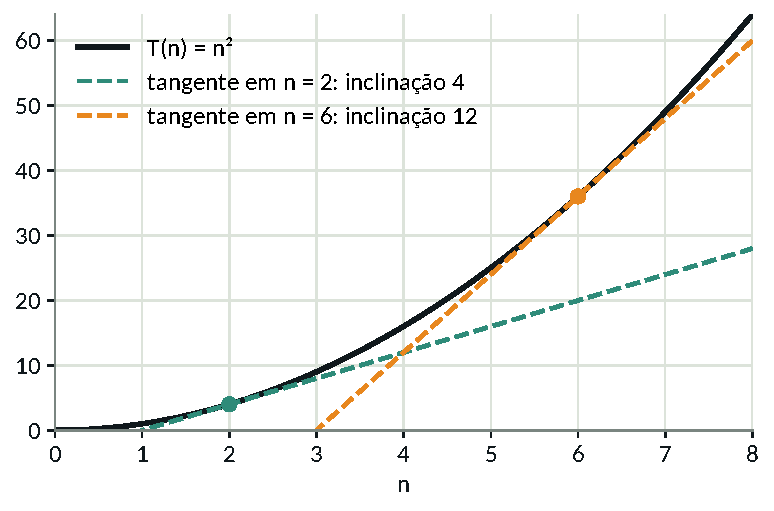
\includegraphics[width=0.72\textwidth]{figuras/f11_tangentes.pdf}
  \caption{Em $T(n) = n^2$, a tangente em $n = 2$ tem inclinação 4; em $n = 6$, inclinação 12.
  Quanto mais à direita, mais íngreme: o crescimento acelera.}
\end{figure}

Escrevemos a derivada de $T(n)$ como $T'(n)$ (lê-se \enquote{tê linha de ene}). Se $T'(n)$ é
constante, a função cresce sempre no mesmo ritmo (é linear); se $T'(n)$ aumenta com $n$, o
crescimento acelera.

\section{A regra da potência}

Para as funções que aparecem em análise de algoritmos, uma regra resolve quase tudo:

\begin{center}
\colorbox{edtealclaro}{\large\quad $\dfrac{d}{dn}\left(n^p\right) = p \cdot n^{p-1}$\quad}
\qquad \small (\enquote{o expoente desce multiplicando e diminui 1})
\end{center}

\begin{center}
\begin{tabularx}{\textwidth}{P{3.4cm} P{3.6cm} L}
\cab \tc{Função} & \tc{Derivada} & \tc{Como} \\
$n$ & $1$ & $n = n^1 \to 1 \cdot n^0 = 1$ \\
\rowcolor{edfundo} $n^2$ & $2n$ & $2 \cdot n^1$ \\
$n^3$ & $3n^2$ & $3 \cdot n^2$ \\
\rowcolor{edfundo} $\sqrt{n} = n^{1/2}$ & $\dfrac{1}{2\sqrt{n}}$ & $\tfrac{1}{2} \cdot n^{-1/2}$ \\
$\dfrac{1}{n} = n^{-1}$ & $-\dfrac{1}{n^2}$ & $-1 \cdot n^{-2}$ \\
\rowcolor{edfundo} uma constante, como $7$ & $0$ & constantes não variam \\
\end{tabularx}
\end{center}

Duas regras completam o kit: a derivada de uma \textbf{soma} é a soma das derivadas, e uma
\textbf{constante multiplicando} continua multiplicando. Por exemplo:
$\dfrac{d}{dn}\left(3n^2 + 5n + 2\right) = 3 \cdot 2n + 5 \cdot 1 + 0 = 6n + 5$.

\subsection{A regra da cadeia para \texorpdfstring{$u^p$}{u elevado a p}}

Quando o que está elevado a $p$ não é o próprio $n$, mas uma expressão $u$ que depende de $n$,
multiplicamos também pela derivada de $u$:
\[
\frac{d}{dn}\left(u^p\right) = p \cdot u^{p-1} \cdot u'
\]
Exemplos: $\dfrac{d}{dn}(n + 1)^2 = 2(n + 1) \cdot 1 = 2n + 2$ \quad e \quad
$\dfrac{d}{dn}(3n - 2)^2 = 2(3n - 2) \cdot 3 = 18n - 12$.

\section{Custo marginal: quanto custa um elemento a mais?}

A derivada responde a uma pergunta prática: \textbf{se o problema ganhar um elemento, quanto
trabalho a mais o algoritmo terá?}

No pior caso do Insertion Sort, $T(n) = \dfrac{n(n-1)}{2} = \dfrac{n^2}{2} - \dfrac{n}{2}$.
Pela regra da potência:
\[
T'(n) = \frac{2n}{2} - \frac{1}{2} = n - \frac{1}{2} \approx n.
\]
Cada elemento a mais custa cerca de $n$ comparações extras. Conferindo com a conta exata:
$T(n + 1) - T(n) = \dfrac{(n+1)n}{2} - \dfrac{n(n-1)}{2} = n$. Para um vetor de 1.000 elementos,
acrescentar mais um custa cerca de 1.000 comparações; para 1.000.000 de elementos, cerca de um
milhão.

Compare com a busca linear, $T(n) = n$: $T'(n) = 1$. Cada elemento a mais custa sempre a mesma
coisa, uma comparação. \textbf{Derivada constante significa crescimento linear; derivada que
cresce significa crescimento acelerado.}

\section{Achando o melhor parâmetro: a busca por saltos}

Agora um problema em que a derivada \emph{resolve} uma questão de projeto.

Queremos procurar um valor num vetor \textbf{ordenado} com $n$ elementos — por exemplo, uma
lista de chamada com 10.000 nomes em ordem alfabética. A busca linear faria até 10.000
comparações. A \textbf{busca por saltos} aproveita a ordem e o acesso por índice em $O(1)$ da
lista contígua (Aula 1):

\begin{enumerate}
  \item Salte de $m$ em $m$ posições, olhando só o último elemento de cada bloco, até achar um
        bloco cujo último elemento seja maior ou igual ao valor procurado.
  \item Faça uma busca linear só dentro desse bloco.
\end{enumerate}

\begin{figure}[!htb]
\centering
\begin{tikzpicture}[scale=0.42]
  \foreach \i in {0,...,23} \draw[fill=white, draw=edcinzaclaro, line width=0.7pt] (\i, 0) rectangle ++(0.9, 0.9);
  \foreach \b in {3,7,11,15} \draw[fill=edtealclaro, draw=edteal, line width=0.9pt] (\b, 0) rectangle ++(0.9, 0.9);
  \foreach \i in {16,...,19} \draw[fill=edlaranjaclaro, draw=edlaranja, line width=0.9pt] (\i, 0) rectangle ++(0.9, 0.9);
  \foreach \a/\b in {-1/3, 3/7, 7/11, 11/15, 15/19}
    \draw[-{Latex}, edteal, line width=1pt] (\a+0.45, 1.1) to[bend left=40] (\b+0.45, 1.1);
  \node[font=\small, color=edteal, anchor=south] at (8, 2.4) {fase 1: saltos de $m = 4$ posições};
  \node[font=\small, color=edlaranja, anchor=north] at (17.9, -0.3) {fase 2: busca linear no bloco};
\end{tikzpicture}
\caption{Busca por saltos com $m = 4$: os saltos examinam o fim de cada bloco (verde); o valor
está no bloco laranja, percorrido um a um.}
\end{figure}

Qual o melhor tamanho de salto $m$? Se $m$ for muito pequeno, damos saltos demais; se for muito
grande, o bloco final é enorme. No pior caso, fazemos cerca de $n/m$ saltos mais $m$ comparações
dentro do bloco:
\[
T(m) = \frac{n}{m} + m.
\]

\begin{figure}[!htb]
  \centering
  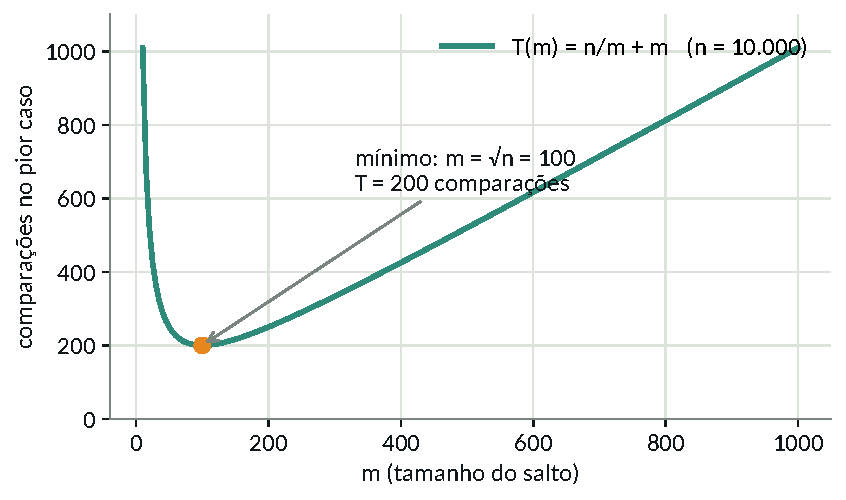
\includegraphics[width=0.72\textwidth]{figuras/f11_busca_saltos.pdf}
  \caption{$T(m)$ para $n = 10.000$: a curva tem um \enquote{vale}. O ponto mais baixo é o melhor
  salto.}
\end{figure}

No ponto mais baixo do vale, a curva fica \enquote{deitada}: a tangente é horizontal, com
inclinação zero. Então basta achar onde $T'(m) = 0$. Escrevendo $\dfrac{n}{m} = n \cdot m^{-1}$ e
usando a regra da potência com $p = -1$:
\[
T'(m) = n \cdot (-1) \cdot m^{-2} + 1 = -\frac{n}{m^2} + 1.
\]
\[
T'(m) = 0 \;\Longleftrightarrow\; \frac{n}{m^2} = 1 \;\Longleftrightarrow\; m^2 = n
\;\Longleftrightarrow\; \boxed{m = \sqrt{n}}.
\]

Com $n = 10.000$: $m = 100$, e o pior caso fica em $T = 100 + 100 = 200$ comparações — contra
10.000 da busca linear. Em geral, $T(\sqrt{n}) = 2\sqrt{n}$: a busca por saltos é $O(\sqrt{n})$.

O programa \codigo{python/busca_saltos.py} testa todos os saltos de 1 a 1.000 e confirma:

\needspace{18\baselineskip}
\lstinputlisting[style=terminal]{tabelas/saida_saltos.txt}

Repare na penúltima linha: vinte valores de $m$, de 91 a 110, empatam em 200. Perto do mínimo,
a curva é quase plana — exatamente o que significa \enquote{inclinação zero}.

\begin{aprofunde}
Como saber que $m = \sqrt{n}$ é um mínimo, e não um máximo? Pela \textbf{segunda derivada}
(a derivada da derivada): $T''(m) = \dfrac{2n}{m^3}$, que é positiva para $m > 0$. Segunda
derivada positiva quer dizer que a inclinação está aumentando: a curva tem a forma de um vale,
e o ponto de inclinação zero é o fundo.
\end{aprofunde}

\section{Comparando crescimentos com limites}

\begin{aprofunde}
Às vezes não é óbvio qual de duas funções cresce mais rápido. Por exemplo: $n \log n$ ou
$n^{1{,}5} = n\sqrt{n}$? Uma técnica é olhar o limite da divisão entre elas quando $n \to \infty$
(capítulo 3): se tende a 0, a de cima cresce mais devagar.

Dividindo as duas por $n$, sobra comparar $\ln n$ com $\sqrt{n}$. As duas vão para o infinito, e
aí entra a \textbf{regra de L'Hôpital}: nesse caso, o limite da divisão é igual ao limite da
divisão das derivadas.
\[
\lim_{n \to \infty} \frac{\ln n}{n^{1/2}}
\;=\; \lim_{n \to \infty} \frac{1/n}{\tfrac{1}{2} n^{-1/2}}
\;=\; \lim_{n \to \infty} \frac{2}{\sqrt{n}} \;=\; 0.
\]
Conclusão: $n \log n$ cresce mais devagar que $n\sqrt{n}$. (Usamos que a derivada de $\ln n$ é
$1/n$.) É por isso que, na hierarquia do capítulo 10, $n \log n$ vem antes de $n^2$, e até
antes de $n^{1{,}5}$.
\end{aprofunde}

\begin{exrapido}
Calcule as derivadas: (a) $n^4$; (b) $5n^2$; (c) $\sqrt{n}$; (d) $\dfrac{1}{n^2}$;
(e) $(n + 1)^2$; (f) $(3n - 2)^2$.
\end{exrapido}

\begin{exrapido}
Na busca por saltos: (a) com $n = 400$, qual é o melhor salto e quantas comparações são feitas
no pior caso? (b) E com $n = 1.000.000$? Compare com a busca linear.
\end{exrapido}

\begin{exrapido}
Um algoritmo faz $T(n) = n^2 + 3n$ passos. Use a derivada para estimar quantos passos a mais ele
faz quando $n$ passa de 100 para 101. Confira calculando $T(101) - T(100)$.
\end{exrapido}

\begin{respostas}
  \resp{11.1} (a) $4n^3$. (b) $10n$. (c) $\dfrac{1}{2\sqrt{n}}$. (d) $n^{-2} \to -2n^{-3} = -\dfrac{2}{n^3}$.
  (e) $2(n + 1)$. (f) $2(3n - 2) \cdot 3 = 18n - 12$.
  \resp{11.2} (a) $m = \sqrt{400} = 20$; $T = 400/20 + 20 = 40$ comparações (contra 400).
  (b) $m = 1.000$; $T = 2.000$ comparações (contra 1.000.000).
  \resp{11.3} $T'(n) = 2n + 3$, então $T'(100) = 203$ passos a mais, aproximadamente. Exato:
  $T(101) - T(100) = (10.201 + 303) - (10.000 + 300) = 204$. A derivada acerta por pouco.
\end{respostas}
}{}
\IfFileExists{capitulos/cap12.tex}{% =====================================================================
\chapter{Regras práticas para analisar código}\label{cap:12}
\naaula{46}

Contar cada passo, como no capítulo 2, é ótimo para aprender — mas trabalhoso. Na prática,
reconhecemos alguns \textbf{padrões} e chegamos direto à notação $O$ (ou $\Theta$).

\section{Os padrões}

\begin{center}
\begin{tabularx}{\textwidth}{P{4.3cm} P{5.2cm} L}
\cab \tc{Padrão} & \tc{Exemplo} & \tc{Custo} \\
comandos simples, sem laço & \codigo{x = v[0] + 1} & $\Theta(1)$ \\
\rowcolor{edfundo} um laço de $n$ voltas com corpo $\Theta(1)$ & \codigo{for i in range(n): soma += v[i]} & $\Theta(n)$ \\
laço dentro de laço, $n$ voltas cada & \codigo{for i ... for j ...} & $\Theta(n^2)$ \\
\rowcolor{edfundo} laço \enquote{triangular}: o de dentro vai até \codigo{i} & \codigo{for i in range(n): for j in range(i)} & $\Theta(n^2)$ (Gauss) \\
laço que divide (ou multiplica) por 2 & \codigo{while i > 1: i //= 2} & $\Theta(\log n)$ \\
\rowcolor{edfundo} blocos em sequência & bloco $A$ e depois bloco $B$ & soma: fica o maior \\
\codigo{if}/\codigo{else} & ramo $A$ ou ramo $B$ & o pior dos ramos (para $O$) \\
\rowcolor{edfundo} chamada de função dentro de laço & $n$ chamadas de algo $\Theta(m)$ & $\Theta(n \cdot m)$ \\
\end{tabularx}
\end{center}

\begin{intuicao}
Duas perguntas resolvem quase tudo: \textbf{quantas vezes cada laço roda?} e \textbf{o que está
dentro de quê?} Laços um \emph{depois} do outro somam; laços um \emph{dentro} do outro multiplicam.
\end{intuicao}

\section{Exemplos resolvidos}

\needspace{10\baselineskip}\textbf{Exemplo 1 — laços em sequência e aninhados.}

\begin{lstlisting}
for i in range(n):          # bloco A: n * n voltas
    for j in range(n):
        print(i, j)
for k in range(n):          # bloco B: n voltas
    print(k)
\end{lstlisting}

O bloco A custa $n^2$; o B, $n$. Em sequência, somam: $n^2 + n$. Fica o termo dominante:
$\Theta(n^2)$.

\needspace{10\baselineskip}\textbf{Exemplo 2 — dividindo ao meio.}

\begin{lstlisting}
i = n
while i > 1:
    i = i // 2
\end{lstlisting}

A cada volta, \codigo{i} cai pela metade: o laço roda cerca de $\log_2 n$ vezes. Custo:
$\Theta(\log n)$.

\needspace{10\baselineskip}\textbf{Exemplo 3 — o laço triangular.}

\begin{lstlisting}
for i in range(n):
    for j in range(i):      # 0, 1, 2, ..., n-1 voltas
        print(i, j)
\end{lstlisting}

O laço de dentro dá $0 + 1 + 2 + \dots + (n - 1) = \dfrac{n(n-1)}{2}$ voltas no total (Gauss).
Custo: $\Theta(n^2)$ — a metade de um quadrado continua quadrática.

\needspace{10\baselineskip}\textbf{Exemplo 4 — um laço logarítmico dentro de um linear.}

\begin{lstlisting}
for i in range(n):          # n voltas
    j = 1
    while j < n:            # cerca de log2(n) voltas
        j = j * 2
\end{lstlisting}

Para cada uma das $n$ voltas de fora, o de dentro roda cerca de $\log_2 n$ vezes. Aninhados,
multiplicam: $\Theta(n \log n)$.

\needspace{10\baselineskip}\textbf{Exemplo 5 — a função escondida.}

\begin{lstlisting}
def comuns(a, b):           # a tem n elementos, b tem m
    resultado = []
    for x in a:             # n voltas
        if x in b:          # "in" percorre b: O(m)
            resultado.append(x)
    return resultado
\end{lstlisting}

O \codigo{x in b} parece um teste simples, mas é uma busca linear em \codigo{b}
(capítulo 2). São $n$ buscas de custo $m$: $O(n \cdot m)$. É a interseção ingênua da Aula 3.

\begin{atencao}
Em Python, desconfie de toda linha que opera sobre uma lista inteira: \codigo{in},
\codigo{insert(0, x)}, \codigo{remove(x)}, \codigo{index(x)}, \codigo{min}, \codigo{max},
\codigo{sum}, \codigo{sorted}. Cada uma esconde um laço.
\end{atencao}

\begin{exrapido}[14]
Dê o custo de cada trecho, em notação $O$.

\begin{lstlisting}
# (a)
for i in range(n):
    for j in range(10):
        print(i, j)
# (b)
i = 1
while i < n:
    i = i * 3
# (c)
for i in range(n):
    lista.insert(0, i)      # lista contígua do Python
\end{lstlisting}
\end{exrapido}

\begin{respostas}
  \resp{12.1} (a) O laço de dentro tem sempre 10 voltas (uma constante): $10n$, ou seja, $O(n)$.
  (b) \codigo{i} é multiplicado por 3 a cada volta: $\log_3 n$ voltas, ou seja, $O(\log n)$ (a
  base não importa). (c) Cada \codigo{insert(0, i)} desloca todos os elementos já inseridos:
  $0 + 1 + \dots + (n - 1)$ deslocamentos, ou seja, $O(n^2)$.
\end{respostas}
}{}
\IfFileExists{capitulos/cap13.tex}{% =====================================================================
\chapter{Revisitando Lista, Pilha, Fila e Conjunto}\label{cap:13}
\naaula{47}

Com as ferramentas desta apostila, podemos olhar de novo para as estruturas das Aulas 1 a 3 e
dizer, com precisão, quanto custa cada operação. Esta tabela é um ótimo resumo para a prova.

\begin{center}
\begin{tabularx}{\textwidth}{P{3.3cm} P{4.2cm} C L}
\cab \tc{Estrutura} & \tc{Operação} & \tc{Custo} & \tc{Por quê} \\
Lista contígua (Aula 1)
  & \codigo{obter(pos)} & $\Theta(1)$ & acesso direto por índice \\
  & inserir/remover no fim & $\Theta(1)$\,* & nada a deslocar \\
  & inserir/remover no início & $\Theta(n)$ & desloca todos \\
  & \codigo{buscar(valor)} & $O(n)$ & melhor caso $\Theta(1)$, pior $\Theta(n)$ \\
\rowcolor{edfundo} Lista encadeada (Aula 1)
  & inserir/remover no início & $\Theta(1)$ & só troca referências \\
\rowcolor{edfundo}  & inserir no fim, com ponteiro \codigo{fim} & $\Theta(1)$ & vai direto ao último nó \\
\rowcolor{edfundo}  & \codigo{obter(pos)} & $O(n)$ & precisa percorrer os nós \\
\rowcolor{edfundo}  & \codigo{buscar(valor)} & $O(n)$ & percorre até achar \\
Pilha contígua (Aula 2)
  & empilhar, desempilhar & $\Theta(1)$ & só mexe no topo \\
  & \codigo{consultar_topo()} & $\Theta(1)$ & acesso direto ao topo \\
\rowcolor{edfundo} Fila encadeada (Aula 2)
  & enfileirar (com ponteiro \codigo{fim}) & $\Theta(1)$ & insere direto no fim \\
\rowcolor{edfundo}  & desenfileirar & $\Theta(1)$ & remove direto do início \\
Conjunto sobre lista (Aula 3)
  & \codigo{pertence(valor)} & $O(n)$ & percorre os elementos \\
  & \codigo{inserir(valor)}, \codigo{remover} & $O(n)$ & chamam \codigo{pertence()} \\
  & união, interseção, diferença & $O(n \cdot m)$ & um \codigo{pertence()} por elemento \\
\rowcolor{edfundo} \codigo{set()} do Python & \codigo{in}, \codigo{add}, \codigo{remove} & $O(1)$\,** & tabela de dispersão \\
\end{tabularx}
\end{center}
{\small * Com espaço disponível (ou, na \codigo{list} do Python, em média).
** Em média; usa uma estrutura chamada tabela de dispersão (\emph{hash}), assunto de um curso mais
adiante.}

\section{A reflexão da Aula 2, respondida}

Na atividade da Aula 2, a pergunta era: \emph{por que manter um ponteiro para o fim permite
enfileirar em $O(1)$? O que mudaria se a fila guardasse apenas o início?}

Com o ponteiro \codigo{fim}, enfileirar é ir direto ao último nó e ligar o novo: um número fixo de
passos, $\Theta(1)$. Sem ele, para achar o último nó seria preciso percorrer a fila inteira a
partir do início: $\Theta(n)$ por enfileiramento. E enfileirar $n$ elementos, um a um, custaria
$0 + 1 + \dots + (n - 1) = \Theta(n^2)$ — Gauss mais uma vez. No Campo Minado (capítulo 14), a
abertura em cascata enfileira até $L \cdot C$ células: com a Fila sem \codigo{fim}, ela passaria
de $O(L \cdot C)$ para $O((L \cdot C)^2)$.

\section{Escolhendo a estrutura}

\begin{itemize}
  \item Precisa acessar por posição com frequência? \textbf{Lista contígua}.
  \item Insere e remove muito no início, e raramente acessa por posição? \textbf{Lista encadeada}.
  \item O último a entrar é o primeiro a sair (desfazer, histórico, navegação)? \textbf{Pilha}.
  \item Atendimento por ordem de chegada (impressão, processos, abertura em ondas)? \textbf{Fila}.
  \item Muitas perguntas \enquote{este valor está aqui?} e nada de duplicatas? \textbf{Conjunto} — e,
        se forem muitas consultas, um \codigo{set()} com custo $O(1)$ em média.
\end{itemize}

\begin{exrapido}
Qual estrutura você usaria, e com que custo por operação, para: (a) o botão \enquote{voltar} de um
navegador; (b) os pedidos de uma lanchonete, atendidos por ordem de chegada; (c) verificar, milhares
de vezes, se um CPF já foi cadastrado?
\end{exrapido}

\begin{respostas}
  \resp{13.1} (a) Pilha: a última página visitada é a primeira a voltar; empilhar e desempilhar
  em $\Theta(1)$. (b) Fila: enfileirar e desenfileirar em $\Theta(1)$, com ponteiro para o fim.
  (c) Um conjunto; com muitas consultas, o \codigo{set()} do Python, com \codigo{in} em $O(1)$ em
  média. Com o Conjunto sobre lista da Aula 3, cada consulta custaria $O(n)$.
\end{respostas}
}{}
\IfFileExists{capitulos/cap14.tex}{% =====================================================================
\chapter{Campo Minado: regras do jogo e técnicas de implementação}\label{cap:14}
\naaula{48}

A atividade prática desta aula é um Campo Minado completo, que usa as estruturas das Aulas 1 a 3
e as análises da Aula 4. Este capítulo explica as regras do jogo em detalhes e cada técnica usada
na solução de exemplo (pasta \codigo{solucoes/campo_minado/} do repositório). Os trechos de
código são da solução real; o enunciado da atividade diz o que você deve implementar.

\section{As regras do jogo}

\subsection{O tabuleiro}

O jogo acontece num tabuleiro de $L$ linhas e $C$ colunas de \textbf{células}. Algumas células —
$k$ delas — escondem uma \textbf{mina}. No começo, todas estão \textbf{fechadas}: o jogador não
sabe onde estão as minas. O objetivo é \textbf{abrir todas as células que não têm mina}.

\begin{center}
\begin{tabularx}{0.8\textwidth}{L C C C}
\cab \tc{Nível} & \tc{Linhas × colunas} & \tc{Células} & \tc{Minas} \\
Fácil & $9 \times 9$ & 81 & 10 \\
\rowcolor{edfundo} Médio & $16 \times 16$ & 256 & 40 \\
Difícil & $16 \times 30$ & 480 & 99 \\
\end{tabularx}
\end{center}

\subsection{Os números}

Ao abrir uma célula sem mina, ela mostra um \textbf{número}: quantas minas existem entre as suas
\textbf{vizinhas} — as até 8 células que encostam nela, inclusive nas diagonais. Uma célula no
meio do tabuleiro tem 8 vizinhas; numa borda, 5; num canto, 3. Os números são as pistas do jogo:
um 1 cercado de células abertas, com uma única vizinha fechada, garante que essa vizinha é mina.

\begin{figure}[!htb]
\centering
\begin{tikzpicture}[scale=0.62]
  \fill[edfundo] (0,0) rectangle (5,5);
  \draw[edcinzaclaro, line width=0.8pt] (0,0) grid (5,5);
  \draw[edverde, line width=1.2pt] (0,0) rectangle (5,5);
  \foreach \i in {1,...,5} {
    \node[font=\small\bfseries, color=edverde] at (\i-0.5, 5.4) {\i};
    \node[font=\small\bfseries, color=edverde] at (-0.4, 5.5-\i) {\i};
  }
  \foreach \c/\l in {1/1, 2/1, 5/1, 1/2, 4/2, 5/2, 1/3, 2/3, 3/3, 4/3, 5/3, 4/4, 4/5, 5/5}
    \node[font=\bfseries, color=edteal] at (\c-0.5, 5.5-\l) {1};
  \foreach \c/\l in {3/1, 3/2}
    \node[font=\bfseries, color=edlaranja] at (\c-0.5, 5.5-\l) {2};
  \foreach \c/\l in {1/4, 2/4, 3/4, 1/5, 2/5, 3/5}
    \node[font=\bfseries, color=edcinza] at (\c-0.5, 5.5-\l) {0};
  \foreach \c/\l in {4/1, 2/2, 5/4} {
    \fill[edtexto] (\c-0.5, 5.5-\l) circle (0.2);
    \foreach \a in {0,45,90,135} \draw[edtexto, line width=1pt] ($(\c-0.5, 5.5-\l)+(\a:0.32)$) -- ($(\c-0.5, 5.5-\l)+(\a+180:0.32)$);
  }
\end{tikzpicture}
\caption{O tabuleiro 5 × 5 da atividade (Parte A), com minas em (1,\,4), (2,\,2) e (4,\,5) e os
números de todas as células seguras.}
\end{figure}

\subsection{A abertura em cascata}

Uma célula com \textbf{0} não tem nenhuma mina em volta. Então todas as suas vizinhas são
seguras, e o jogo as abre automaticamente. Se alguma delas também for 0, as vizinhas dela também
se abrem, e assim por diante: uma única jogada pode abrir uma área grande. As células numeradas
formam a \enquote{borda} da área aberta: elas se abrem, mas não espalham a abertura.

\subsection{Bandeiras, primeiro clique, vitória e derrota}

\begin{itemize}
  \item \textbf{Bandeira:} o jogador pode marcar uma célula fechada onde acha que há mina. A
        célula marcada não pode ser aberta (nem pela cascata) até a bandeira ser retirada. O placar
        mostra \enquote{minas menos bandeiras}; ele fica negativo se houver bandeiras demais.
  \item \textbf{Primeiro clique seguro:} as minas só são sorteadas depois do primeiro clique,
        longe da célula clicada e das suas vizinhas. Assim, o primeiro clique sempre abre uma área.
  \item \textbf{Derrota:} abrir uma célula com mina. O jogo mostra todas as minas e marca as
        bandeiras colocadas em lugares errados.
  \item \textbf{Vitória:} abrir todas as células seguras. As minas que faltavam ganham bandeira.
  \item \textbf{Desfazer:} só a última bandeira pode ser desfeita. Abrir uma célula não tem volta.
\end{itemize}

\subsection{Como jogar nas duas interfaces}

Na \textbf{interface gráfica} (\codigo{jogo_gui.py}): clique esquerdo abre, clique direito (no Mac,
Control + clique) marca bandeira, \textbf{Ctrl+Z} desfaz a última bandeira e \textbf{F2} começa um
novo jogo. O menu \textbf{Análise} permite escolher Fila ou Pilha para a cascata, animar a abertura,
numerar a ordem de abertura e ver o painel com as operações contadas. Na \textbf{interface de
texto} (\codigo{jogo_terminal.py}), os comandos são \codigo{r 3 5} (revelar a linha 3, coluna 5),
\codigo{b 3 5} (bandeira), \codigo{d} (desfazer), \codigo{h} (histórico), \codigo{o} (operações),
\codigo{a} (alternar Fila e Pilha) e \codigo{s} (sair).

\begin{figure}[!htb]
  \centering
  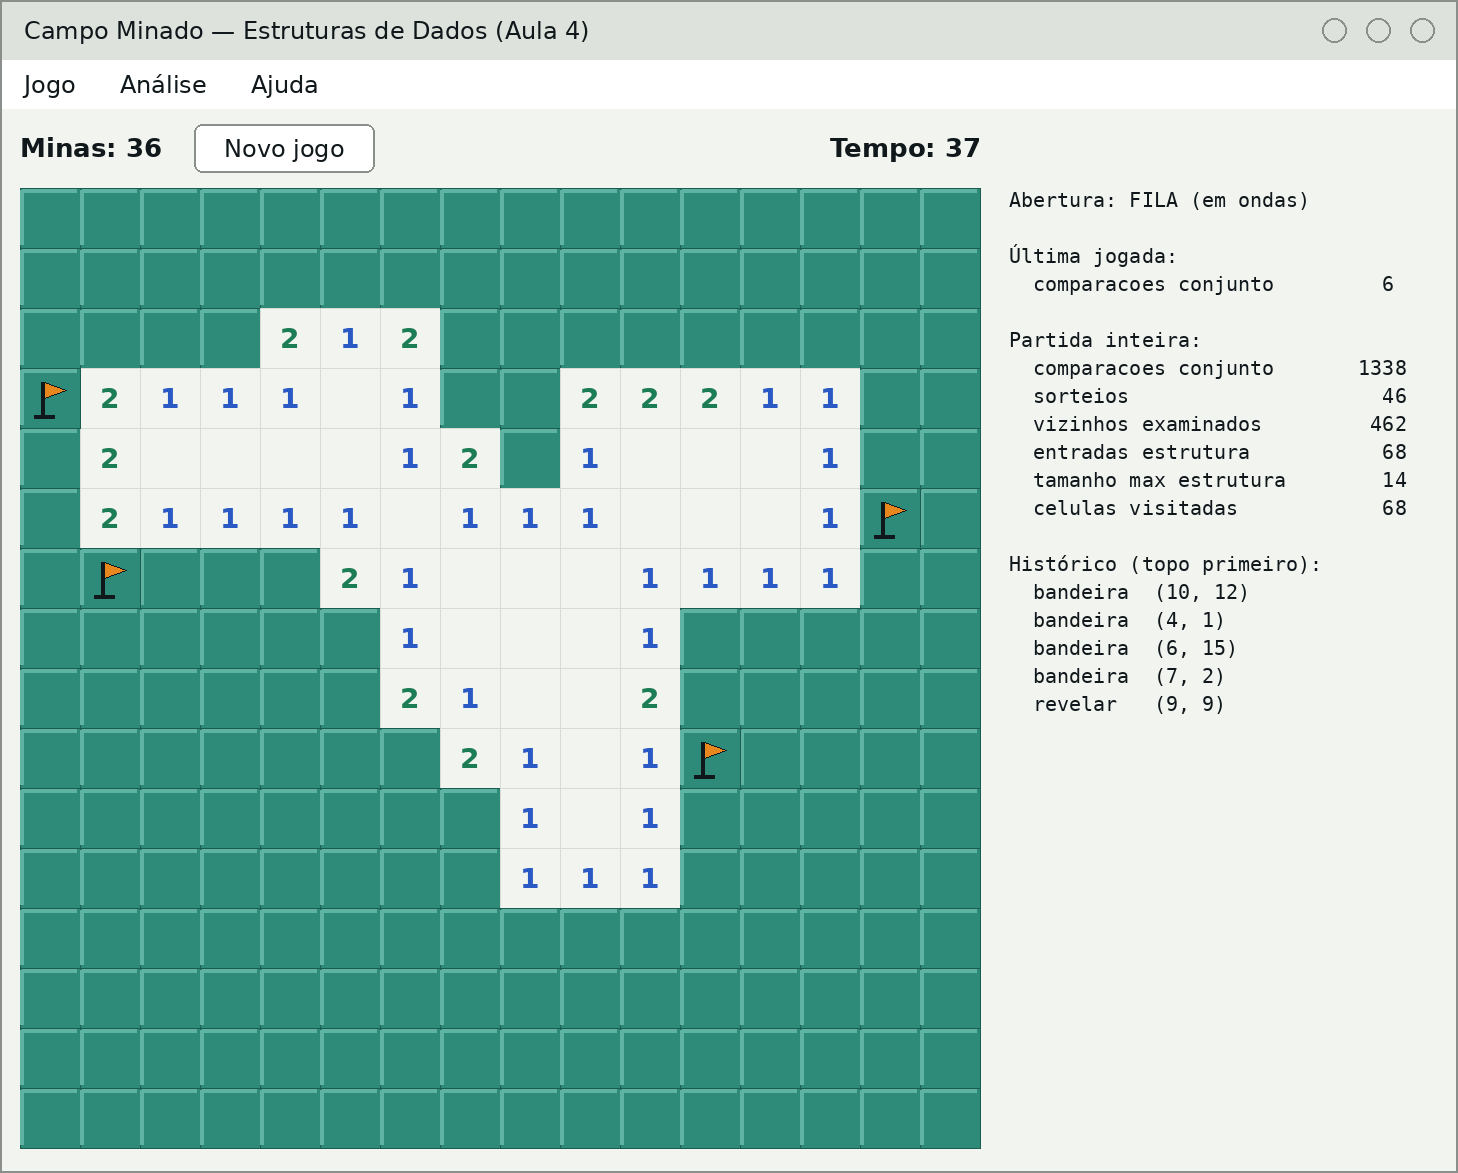
\includegraphics[width=0.78\textwidth]{figuras/janela_campo_minado.png}
  \caption{A interface gráfica, com o painel de análise (ilustração gerada a partir do código de
  desenho do jogo).}
\end{figure}

\section{A organização do programa}

A decisão de projeto mais importante é \textbf{separar a lógica da interface}. Todas as regras
ficam na classe \codigo{Tabuleiro}, que não imprime nada nem abre janelas. As interfaces só
chamam os métodos dela e desenham o resultado.

\begin{figure}[!htb]
\centering
\begin{tikzpicture}[caixa/.style={draw=edteal, fill=edtealclaro, line width=1pt, rounded corners=2pt,
    minimum width=3.1cm, minimum height=0.9cm, font=\small, align=center},
    seta/.style={-{Latex}, line width=1pt, edverde}]
  \node[caixa] (e) at (0,0) {\texttt{estruturas.py}\\Pilha, Fila, Conjunto};
  \node[caixa, fill=edlaranjaclaro, draw=edlaranja] (t) at (0,-1.7) {\texttt{tabuleiro.py}\\regras do jogo};
  \node[caixa] (r) at (4.4,-1.7) {\texttt{ranking.py}\\melhores tempos};
  \node[caixa] (gui) at (-4.4,-3.5) {\texttt{jogo\_gui.py}\\janela (tkinter)};
  \node[caixa] (ter) at (-1.2,-3.5) {\texttt{jogo\_terminal.py}\\texto};
  \node[caixa] (tes) at (2.0,-3.5) {\texttt{testes.py}\\testes automáticos};
  \node[caixa] (an) at (5.2,-3.5) {\texttt{analise\_...py}\\medições};
  \draw[seta] (e) -- (t);
  \foreach \x in {gui, ter, tes, an} \draw[seta] (\x.north) -- (t.south);
  \draw[seta] (gui.north) to[bend left=35] (r.north west);
  \draw[seta] (ter.north) -- (r.south west);
\end{tikzpicture}
\caption{Quem usa quem: as setas apontam para o módulo usado. As regras ficam num único lugar.}
\end{figure}

Vantagens: a mesma lógica serve às duas interfaces; os testes verificam as regras sem abrir
janela nenhuma; e dá para trocar a interface sem mexer nas regras (e vice-versa).

\section{Técnica 1: o tabuleiro numa lista linear}

Um tabuleiro parece pedir uma matriz, mas a solução guarda tudo em \textbf{listas lineares}, com
uma posição por célula — a lista contígua da Aula 1. A célula (linha, coluna) fica na posição
\[
\text{índice} = \text{linha} \times C + \text{coluna} \qquad \text{(contando a partir de 0)}.
\]

\begin{figure}[!htb]
\centering
\begin{tikzpicture}[scale=0.62]
  \foreach \l in {0,1,2} \foreach \c in {0,...,3} {
    \pgfmathtruncatemacro{\idx}{\l*4+\c}
    \draw[fill=edtealclaro, draw=edteal, line width=0.8pt] (\c, -\l) rectangle ++(0.95,0.95);
    \node[font=\small] at (\c+0.47, -\l+0.47) {\idx};
  }
  \node[font=\small, color=edcinza] at (1.9, 1.4) {tabuleiro 3 × 4};
  \foreach \i/\cor in {0/edtealclaro, 1/edtealclaro, 2/edtealclaro, 3/edtealclaro,
                      4/edlaranjaclaro, 5/edlaranjaclaro, 6/edlaranjaclaro, 7/edlaranjaclaro,
                      8/edfundo2, 9/edfundo2, 10/edfundo2, 11/edfundo2} {
    \draw[fill=\cor, draw=edteal, line width=0.8pt] (6.2+\i*0.95, -0.9) rectangle ++(0.9,0.9);
    \node[font=\small] at (6.2+\i*0.95+0.45, -0.45) {\i};
  }
  \node[font=\small, color=edcinza] at (11.9, 0.55) {a mesma coisa, numa lista linear};
  \node[font=\footnotesize, color=edteal] at (7.9, -1.5) {linha 0};
  \node[font=\footnotesize, color=edlaranja] at (11.7, -1.5) {linha 1};
  \node[font=\footnotesize, color=edverde] at (15.5, -1.5) {linha 2};
\end{tikzpicture}
\caption{Com 4 colunas, a célula (1,\,2) fica no índice $1 \times 4 + 2 = 6$.}
\end{figure}

\begin{lstlisting}
def indice(self, linha, coluna):
    return linha * self.colunas + coluna                  # O(1)

def coordenadas(self, indice):
    return indice // self.colunas, indice % self.colunas  # O(1)
\end{lstlisting}

Ler ou alterar qualquer célula custa $O(1)$. E um único número identifica cada célula, o que
simplifica guardar células em Conjuntos, Filas e Pilhas.

\section{Técnica 2: vizinhança e bordas}

As 8 direções ficam numa tupla de deslocamentos, sempre na mesma ordem. Para cada uma, calcula-se
a vizinha e descarta-se o que cair fora do tabuleiro:

\begin{lstlisting}
DIRECOES = ((-1, -1), (-1, 0), (-1, 1),     # noroeste, norte, nordeste
            (0, -1),           (0, 1),      # oeste, leste
            (1, -1),  (1, 0),  (1, 1))      # sudoeste, sul, sudeste

def vizinhos(self, indice):
    linha, coluna = self.coordenadas(indice)
    resultado = []
    for delta_linha, delta_coluna in DIRECOES:
        l, c = linha + delta_linha, coluna + delta_coluna
        if 0 <= l < self.linhas and 0 <= c < self.colunas:   # dentro do tabuleiro?
            resultado.append(self.indice(l, c))
    return resultado
\end{lstlisting}

São sempre 8 tentativas: custo $\Theta(1)$. A verificação de bordas é essencial. Sem ela, a
última célula de uma linha \enquote{enxergaria} a primeira célula da linha de baixo, porque na
lista linear elas são vizinhas de posição.

\section{Técnica 3: sortear minas sem repetição}

O sorteio usa o \textbf{Conjunto} da Aula 3, que já ignora valores repetidos:

\begin{lstlisting}
proibidas = Conjunto(self.contador)          # a célula clicada e suas vizinhas
proibidas.inserir(protegida)
for vizinha in self.vizinhos(protegida):
    proibidas.inserir(vizinha)

while self.minas.tamanho() < self.num_minas:
    candidata = self._gerador.randrange(self.total_celulas)
    if not proibidas.pertence(candidata):
        self.minas.inserir(candidata)        # o Conjunto ignora repetidas
\end{lstlisting}

Cada \codigo{inserir()} chama \codigo{pertence()}, que percorre as minas já sorteadas: $0 + 1 +
\dots + (k - 1) = \dfrac{k(k-1)}{2}$ comparações, ou seja, $O(k^2)$ — mais as tentativas
repetidas, que são poucas quando $k$ é pequeno perto do tabuleiro. No nível Difícil, foram 122
tentativas e 6.515 comparações.

\begin{aprofunde}
Uma alternativa sem repetições é o \textbf{embaralhamento de Fisher–Yates}: coloque numa lista os
índices permitidos e, de trás para a frente, troque cada posição com uma posição sorteada entre as
anteriores (inclusive ela). No fim, a lista está embaralhada com todas as ordens igualmente
prováveis, e as primeiras $k$ posições são as minas. Custo: $\Theta(L \cdot C)$, sem nenhuma
repetição. Vale mais a pena quando há muitas minas, caso em que o sorteio simples repetiria muito.
\end{aprofunde}

\section{Técnica 4: calcular os números percorrendo as minas}

A forma óbvia de calcular os números seria perguntar, para cada célula, \enquote{quantas das minhas
vizinhas são minas?}: $L \cdot C$ células, até 8 consultas ao Conjunto cada uma, e cada consulta
custando $O(k)$. Total: $O(L \cdot C \cdot k)$. A solução faz o contrário:

\begin{lstlisting}
for mina in self.minas.valores():            # só as k minas
    for vizinha in self.vizinhos(mina):      # até 8 vizinhas
        self.numeros[vizinha] += 1
\end{lstlisting}

São no máximo 8 passos por mina: $O(k)$. Medido com o \codigo{analise_complexidade.py}:

\begin{center}
\begin{tabularx}{\textwidth}{L C C C C}
\cab \tc{Nível} & \tcx{$L \times C$} & \tcx{$k$} & \tc{Percorrendo as minas} & \tc{Perguntando a cada célula} \\
Fácil & $9 \times 9$ & 10 & 65 & 5.110 \\
\rowcolor{edfundo} Médio & $16 \times 16$ & 40 & 294 & 68.664 \\
Difícil & $16 \times 30$ & 99 & 735 & 317.004 \\
\end{tabularx}
\end{center}

No nível Difícil, a forma ingênua faz cerca de \textbf{431 vezes} mais trabalho para chegar ao
mesmo resultado. Mudar o ponto de vista do algoritmo mudou a família do custo.

\section{Técnica 5: a abertura em cascata com Fila ou Pilha}

A abertura em cascata é um algoritmo clássico de \enquote{preenchimento de região}
(\emph{flood fill}). Ele mantém uma estrutura de células \textbf{pendentes}: retira uma, e, se ela
for 0, coloca na estrutura as vizinhas ainda fechadas.

\begin{lstlisting}
usar_fila = self.estrategia == "fila"
pendentes = Fila() if usar_fila else Pilha(self.total_celulas)
colocar = pendentes.enfileirar if usar_fila else pendentes.empilhar
retirar = pendentes.desenfileirar if usar_fila else pendentes.desempilhar

ordem = []
self._marcar_revelada(inicio)                # marca AO COLOCAR na estrutura
colocar(inicio)
while not pendentes.esta_vazia():
    atual = retirar()
    ordem.append(atual)
    if self.numeros[atual] != 0:
        continue                             # numerada: abre, mas não espalha
    for vizinha in self.vizinhos(atual):
        if not self.reveladas[vizinha] and not self.bandeiras.pertence(vizinha):
            self._marcar_revelada(vizinha)
            colocar(vizinha)
return ordem
\end{lstlisting}

Três detalhes fazem toda a diferença:

\begin{itemize}
  \item \textbf{Funções como valores:} \codigo{colocar} e \codigo{retirar} guardam as operações da
        estrutura escolhida, e o resto do algoritmo é o mesmo para Fila e Pilha.
  \item \textbf{Marcar ao colocar:} a célula é marcada como aberta no momento em que entra na
        estrutura. Assim, cada célula entra no máximo uma vez, e a abertura custa $O(L \cdot C)$.
        Se marcássemos só ao retirar, uma célula poderia entrar uma vez para cada vizinha que a
        visse antes de ela sair:
\end{itemize}

\begin{center}
\begin{tabularx}{0.85\textwidth}{C C C C}
\cab \tcx{$N$} & \tcx{Células ($N^2$)} & \tc{Entradas, marcando ao colocar} & \tc{Entradas, marcando ao retirar} \\
10 & 100 & 100 & 343 \\
\rowcolor{edfundo} 20 & 400 & 400 & 1.483 \\
40 & 1.600 & 1.600 & 6.163 \\
\end{tabularx}
\end{center}
{\small Tabuleiro $N \times N$ sem minas, aberto a partir do canto: o pior caso da cascata.}

\begin{itemize}
  \item \textbf{Fila ou Pilha:} as duas abrem exatamente as mesmas células, com o mesmo custo de
        tempo. Muda a \textbf{ordem}: a Fila abre em ondas a partir do clique (busca em largura);
        a Pilha segue um caminho em profundidade antes de voltar (busca em profundidade).
\end{itemize}

\begin{figure}[!htb]
  \centering
  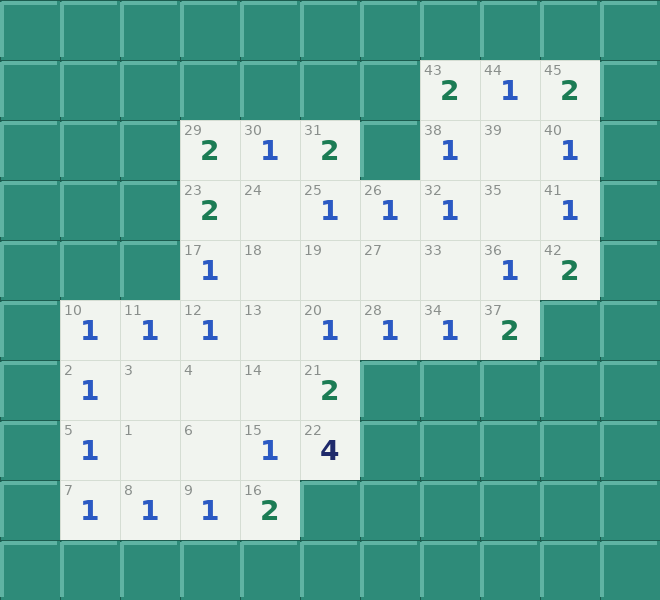
\includegraphics[width=0.45\textwidth]{figuras/ordem_fila.png}\hfill
  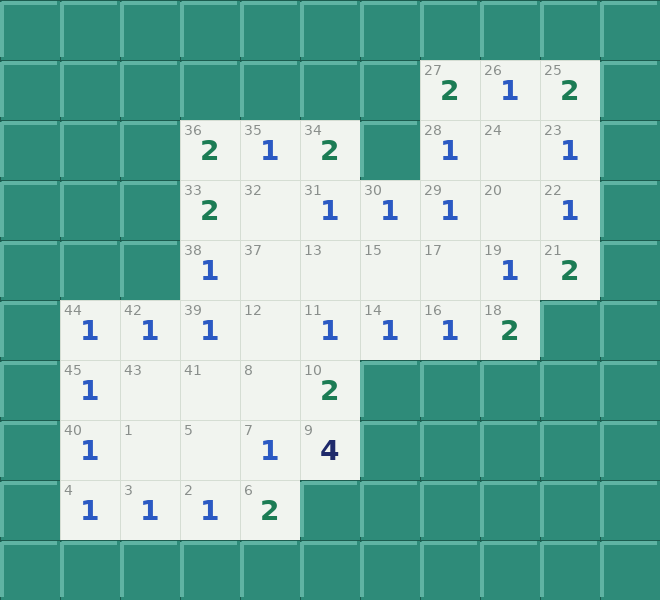
\includegraphics[width=0.45\textwidth]{figuras/ordem_pilha.png}
  \caption{Mesmo tabuleiro, mesmo clique: com Fila (esquerda) e com Pilha (direita). Os números
  pequenos indicam a ordem de abertura.}
\end{figure}

A diferença aparece na \textbf{memória}: a Fila guarda só a \enquote{frente da onda}; a Pilha pode
acumular muito mais células ao mesmo tempo. Por isso a Pilha contígua (de capacidade fixa, como
na Aula 2) é criada com capacidade $L \cdot C$.

\begin{center}
\begin{tabularx}{0.85\textwidth}{C C C C}
\cab \tcx{$N$} & \tc{Células} & \tc{Maior tamanho da Fila} & \tc{Maior tamanho da Pilha} \\
10 & 100 & 19 & 44 \\
\rowcolor{edfundo} 20 & 400 & 39 & 142 \\
40 & 1.600 & 79 & 487 \\
\rowcolor{edfundo} 80 & 6.400 & 159 & 1.777 \\
\end{tabularx}
\end{center}

\section{Técnica 6: vitória em \texorpdfstring{$O(1)$}{O(1)}}

Para saber se o jogador venceu, poderíamos varrer a lista \codigo{reveladas} a cada jogada:
$O(L \cdot C)$ por jogada. A solução mantém um contador, \codigo{celulas_seguras_restantes}, que
começa em $L \cdot C - k$ e diminui 1 a cada célula aberta. A vitória é simplesmente
\codigo{celulas_seguras_restantes == 0}: $O(1)$. É a mesma ideia do \codigo{tamanho} guardado na
Lista da Aula 1: \textbf{manter uma informação atualizada custa pouco e evita recalcular tudo}.

\section{Técnica 7: histórico com Pilha e o desfazer}

Cada jogada é empilhada como uma tupla \codigo{("revelar", linha, coluna)} ou
\codigo{("bandeira", linha, coluna)}. Desfazer consulta o \textbf{topo}: se for uma bandeira,
desempilha e desfaz; se for um \enquote{revelar}, não faz nada, porque abrir uma célula não tem volta.

\begin{lstlisting}
acao, linha, coluna = self.historico.consultar_topo()
if acao != "bandeira":
    return None                              # revelar não tem volta
self.historico.desempilhar()
\end{lstlisting}

É o comportamento LIFO em ação: só o último elemento é acessível. As \enquote{últimas jogadas}
mostradas no painel são os valores da Pilha do topo para a base, sem remover nada.

\section{Técnica 8: ranking com inserção ordenada}

O ranking guarda os 10 melhores tempos de cada nível numa lista sempre ordenada. Para inserir um
recorde, faz um passo do Insertion Sort: coloca no fim e desloca para a direita os tempos maiores.
Custo $O(n)$ no pior caso e $O(1)$ no melhor. Ao carregar o arquivo, ordena com o Insertion Sort
completo — e, como o próprio programa salva o arquivo já ordenado, cai no \textbf{melhor caso},
$\Theta(n)$, exatamente o cenário do capítulo 9.

\section{Técnica 9: medir contando operações}

A classe \codigo{ContadorOperacoes} registra, por categoria, o trabalho de cada jogada:
\enquote{entradas na estrutura}, \enquote{células visitadas}, \enquote{vizinhos examinados},
\enquote{comparações no Conjunto}. O próprio \codigo{pertence()} do Conjunto conta cada
comparação que faz — por isso ele usa um laço explícito em vez de \codigo{valor in lista}, que
esconderia o trabalho. É a contagem de operações do capítulo 2, aplicada a um programa inteiro.

\section{Técnica 10: interfaces, eventos e testes}

\begin{itemize}
  \item \textbf{Programação orientada a eventos:} a interface gráfica não tem um laço que lê
        comandos. Ela registra funções que o tkinter chama quando algo acontece
        (\codigo{canvas.bind("<Button-1>", ...)} para o clique) e usa \codigo{raiz.after(ms, funcao)}
        para agendar ações no futuro: o relógio e cada quadro da animação da abertura.
  \item \textbf{Desenho com etiquetas:} cada célula desenhada no Canvas recebe a etiqueta
        \codigo{"c<indice>"}, para ser apagada e redesenhada sozinha, sem redesenhar o tabuleiro todo.
  \item \textbf{Testes com semente fixa:} com \codigo{random.Random(semente)}, o sorteio é sempre o
        mesmo, e os testes podem conferir resultados exatos. O \codigo{testes.py} usa o tabuleiro da
        Parte A e confere, por exemplo, a ordem exata de abertura com Fila e com Pilha.
\end{itemize}

\section{Resumo dos custos}

\begin{center}
\begin{tabularx}{\textwidth}{L C L}
\cab \tc{Operação} & \tc{Custo} & \tc{Técnica} \\
\codigo{indice()}, \codigo{coordenadas()}, \codigo{vizinhos()} & $\Theta(1)$ & lista linear, 8 direções \\
\rowcolor{edfundo} sortear as minas & $O(k^2)$ & Conjunto sobre lista \\
calcular os números & $O(k)$ & percorrer as minas \\
\rowcolor{edfundo} abertura em cascata & $O(L \cdot C \cdot f)$ & Fila ou Pilha, marcar ao colocar \\
verificar vitória & $\Theta(1)$ & contador de células seguras \\
\rowcolor{edfundo} bandeira, desfazer & $O(f)$ & Conjunto e Pilha \\
registrar recorde & $O(n)$ & inserção ordenada \\
\end{tabularx}
\end{center}
{\small $f$ = número de bandeiras. Na abertura, cada vizinha examinada consulta o Conjunto de
bandeiras ($O(f)$); com uma lista de booleanos, essa consulta seria $O(1)$ e a abertura,
$O(L \cdot C)$.}

\begin{exrapido}
No tabuleiro 5 × 5 da Parte A (5 colunas, contando a partir de 0 no código): (a) qual é o índice
da célula (3,\,4)? (b) quais são os índices das vizinhas da célula de índice 0? (c) quantas
vizinhas tem a célula de índice 12?
\end{exrapido}

\begin{respostas}
  \resp{14.1} (a) $3 \times 5 + 4 = 19$ — é a mina da linha 4, coluna 5 (contando a partir de 1).
  (b) A célula 0 é o canto superior esquerdo: vizinhas 1, 5 e 6. (c) A célula 12 é
  (2,\,2), no meio do tabuleiro: 8 vizinhas.
\end{respostas}
}{}
\IfFileExists{capitulos/cap15.tex}{% =====================================================================
\chapter{Lista de exercícios resolvidos}\label{cap:15}
\naaula{todos}

Resolva cada exercício antes de olhar a resolução. As estrelas indicam a dificuldade:
{\color{edlaranja}\estrela{}} direto, {\color{edlaranja}\estrela{}\estrela{}} médio, {\color{edlaranja}\estrela{}\estrela{}\estrela{}} desafiador.
O bloco D traz questões objetivas no estilo da prova automática do Grau 1 no LEX.

% =====================================================================
\section{Bloco A — contagem e matemática}

\exercicio{A1}{\estrela{}}
Conte os passos do trecho abaixo e escreva $T(n)$. Quanto vale $T(100)$?
\begin{lstlisting}[style=c]
int s = 0;
for (int i = 0; i < n; i++) {
    s = s + i * i;
}
\end{lstlisting}
\begin{resolucao}
\codigo{s = 0}: 1; \codigo{i = 0}: 1; testes: $n + 1$; corpo: $n$; incrementos: $n$. Total:
$T(n) = 3n + 3$. Para $n = 100$: $T(100) = 303$.
\end{resolucao}

\exercicio{A2}{\estrela{}}
Quantas voltas dá o laço \codigo{for i in range(0, n, 2)} (de 2 em 2)? Qual é o seu custo?
\begin{resolucao}
Ele passa por $0, 2, 4, \dots$: cerca de $n/2$ voltas. Metade de $n$ continua crescendo como $n$
(a constante $1/2$ é desprezada): $\Theta(n)$.
\end{resolucao}

\exercicio{A3}{\estrela{}}
Calcule: (a) $\log_2 512$; (b) $\log_2 2^{20}$; (c) $\log_2 1$; (d) entre quais inteiros está $\log_2 3.000$?
\begin{resolucao}
(a) 9, pois $2^9 = 512$. (b) 20 (o expoente \enquote{desce}). (c) 0, pois $2^0 = 1$.
(d) Entre 11 e 12, pois $2^{11} = 2.048 < 3.000 < 4.096 = 2^{12}$.
\end{resolucao}

\exercicio{A4}{\estrela{}\estrela{}}
Calcule (a) $\displaystyle\sum_{i=1}^{50} i$ \quad e \quad (b) $\displaystyle\sum_{i=1}^{n} (2i + 1)$.
\begin{resolucao}
(a) $\dfrac{50 \cdot 51}{2} = 1.275$. (b) Separando: $2 \sum i + \sum 1 = 2 \cdot \dfrac{n(n+1)}{2} + n
= n^2 + n + n = n^2 + 2n$. Confira com $n = 2$: $3 + 5 = 8 = 4 + 4$.
\end{resolucao}

\exercicio{A5}{\estrela{}\estrela{}}
Uma lista contígua tem $n$ elementos. Removemos sempre o \textbf{primeiro} elemento, até a lista
ficar vazia. Quantos deslocamentos acontecem ao todo? Qual é o custo?
\begin{resolucao}
Remover o primeiro de uma lista com $t$ elementos desloca os $t - 1$ restantes. Somando para
$t = n, n-1, \dots, 1$: $(n-1) + (n-2) + \dots + 0 = \dfrac{n(n-1)}{2}$ deslocamentos: $\Theta(n^2)$.
Com uma Fila encadeada, cada remoção seria $\Theta(1)$ e o total, $\Theta(n)$.
\end{resolucao}

\exercicio{A6}{\estrela{}\estrela{}}
A função \codigo{tem_repetido()} do capítulo 8 recebe uma lista de 10 elementos sem nenhum
valor repetido. Quantas comparações ela faz?
\begin{resolucao}
É o pior caso: todas as duplas são comparadas. $9 + 8 + \dots + 1 + 0 = \dfrac{10 \cdot 9}{2} = 45$.
\end{resolucao}

% =====================================================================
\section{Bloco B — notações}

\exercicio{B1}{\estrela{}}
Mostre que $5n + 3 = O(n)$.
\begin{resolucao}
Com $c = 6$: $5n + 3 \le 6n \Longleftrightarrow n \ge 3$. Então $c = 6$, $n_0 = 3$. (Pela técnica
de somar coeficientes: $5n + 3 \le 8n$ para $n \ge 1$, com $c = 8$, $n_0 = 1$.)
\end{resolucao}

\exercicio{B2}{\estrela{}\estrela{}}
Mostre que $n^3 + 2n^2 = \Theta(n^3)$.
\begin{resolucao}
Piso: $n^3 + 2n^2 \ge n^3$ sempre. Teto: para $n \ge 1$, $2n^2 \le 2n^3$, então
$n^3 + 2n^2 \le 3n^3$. Logo, $c_1 = 1$, $c_2 = 3$ e $n_0 = 1$.
\end{resolucao}

\exercicio{B3}{\estrela{}\estrela{}}
Verdadeiro ou falso? (a) $n = O(n^2)$; (b) $n^2 = O(n)$; (c) $2^{n+1} = O(2^n)$;
(d) $3^n = O(2^n)$; (e) $\log_2 n = O(\log_{10} n)$; (f) $n \log n = O(n^2)$.
\begin{resolucao}
(a) V (teto folgado, mas verdadeiro). (b) F (seção 5.5). (c) V: $2^{n+1} = 2 \cdot 2^n$, basta
$c = 2$. (d) F: $3^n / 2^n = 1{,}5^n$ cresce sem limite; nenhuma constante segura. (e) V: as bases
só diferem por uma constante ($\approx 3{,}32$). (f) V: $\log n \le n$, então $n \log n \le n \cdot n$.
\end{resolucao}

\exercicio{B4}{\estrela{}\estrela{}\estrela{}}
Mostre que $n^2 - 10n = \Omega(n^2)$.
\begin{resolucao}
Tentando $c = \tfrac{1}{2}$: $n^2 - 10n \ge \tfrac{n^2}{2} \Longleftrightarrow \tfrac{n^2}{2} \ge 10n
\Longleftrightarrow n \ge 20$. Então $c = \tfrac{1}{2}$ e $n_0 = 20$.
\end{resolucao}

\exercicio{B5}{\estrela{}}
Dê o $\Theta$ de cada função: (a) $7n^2 + n\log n$; (b) $n + \sqrt{n}$; (c) $2^n + n^{100}$;
(d) $(n+1)(n-1)$; (e) $1.000\log n + 5$.
\begin{resolucao}
(a) $\Theta(n^2)$. (b) $\Theta(n)$. (c) $\Theta(2^n)$ — a exponencial vence qualquer potência,
mesmo $n^{100}$, para $n$ grande o bastante. (d) $n^2 - 1$: $\Theta(n^2)$. (e) $\Theta(\log n)$.
\end{resolucao}

\exercicio{B6}{\estrela{}}
Por que não se escreve $O(2n)$ nem $O(n^2 + n)$?
\begin{resolucao}
Porque $O$ descreve a forma do crescimento: constantes multiplicativas e termos menores não mudam
essa forma. $O(2n)$ e $O(n)$ são o mesmo conjunto de funções; por convenção, usa-se a forma mais
simples: $O(n)$ e $O(n^2)$.
\end{resolucao}

% =====================================================================
\section{Bloco C — casos e algoritmos}

\exercicio{C1}{\estrela{}}
Aplique o Insertion Sort a $[3, 1, 2]$, contando comparações e deslocamentos.
\begin{resolucao}
Passada 1 (chave 1): compara com 3 (desloca) e \codigo{j} chega a $-1$: 1 comparação, 1
deslocamento: $[1, 3, 2]$. Passada 2 (chave 2): compara com 3 (desloca) e com 1 (para):
2 comparações, 1 deslocamento: $[1, 2, 3]$. Total: 3 comparações e 2 deslocamentos (e 2
inversões no vetor original: os pares (3,1) e (3,2)).
\end{resolucao}

\exercicio{C2}{\estrela{}}
Numa busca linear em 99 elementos, com o valor presente e qualquer posição igualmente provável,
quantas comparações são feitas em média?
\begin{resolucao}
$\dfrac{n + 1}{2} = \dfrac{100}{2} = 50$.
\end{resolucao}

\exercicio{C3}{\estrela{}\estrela{}}
Num vetor \textbf{ordenado}, uma busca linear pode parar assim que encontrar um elemento maior
que o valor procurado (ele não pode estar mais à frente). Qual é o melhor e o pior caso?
\begin{resolucao}
Melhor caso: o primeiro elemento já é maior ou igual ao valor: 1 comparação, $\Theta(1)$. Pior
caso: o valor é maior que todos (ou é o último): $n$ comparações, $\Theta(n)$. A parada antecipada
melhora o caso médio quando o valor não está, mas não muda a família do pior caso.
\end{resolucao}

\exercicio{C4}{\estrela{}\estrela{}}
Na busca por saltos com $n = 2.500$, qual é o melhor salto e quantas comparações são feitas no
pior caso?
\begin{resolucao}
$m = \sqrt{2.500} = 50$; $T = 2.500/50 + 50 = 100$ comparações (contra 2.500 da busca linear).
\end{resolucao}

\exercicio{C5}{\estrela{}\estrela{}\estrela{}}
O \textbf{Bubble Sort com parada antecipada} percorre o vetor trocando vizinhos fora de ordem e
para quando uma passada inteira não faz nenhuma troca. Qual é o melhor e o pior caso, em
comparações?
\begin{lstlisting}
def bubble_sort(v):
    n = len(v)
    for fim in range(n - 1, 0, -1):
        trocou = False
        for i in range(fim):
            if v[i] > v[i + 1]:
                v[i], v[i + 1] = v[i + 1], v[i]
                trocou = True
        if not trocou:
            break               # nenhuma troca: já está ordenado
\end{lstlisting}
\begin{resolucao}
Melhor caso (vetor ordenado): a primeira passada faz $n - 1$ comparações, nenhuma troca, e o
algoritmo para: $\Theta(n)$. Pior caso (ordem inversa): todas as passadas acontecem, com
$(n-1) + (n-2) + \dots + 1 = \dfrac{n(n-1)}{2}$ comparações: $\Theta(n^2)$. Mesmo perfil do
Insertion Sort — embora, na prática, o Bubble Sort faça mais trocas.
\end{resolucao}

\exercicio{C6}{\estrela{}\estrela{}}
Uma Fila encadeada guarda só o ponteiro para o início. Qual é o custo de enfileirar $n$ elementos,
um a um, começando da fila vazia?
\begin{resolucao}
Para enfileirar, é preciso percorrer até o último nó: com $t$ elementos, $t$ passos. Total:
$0 + 1 + \dots + (n-1) = \dfrac{n(n-1)}{2}$: $\Theta(n^2)$. Com o ponteiro \codigo{fim}, seria
$\Theta(n)$ no total (capítulo 13).
\end{resolucao}

% =====================================================================
\section{Bloco D — questões objetivas (estilo da prova)}

\exercicio{D1}{\estrela{}}
Qual é o custo de ler \codigo{v[i]} numa lista contígua com $n$ elementos?
\quad (a) $O(n)$ \quad (b) $O(1)$ \quad (c) $O(\log n)$ \quad (d) $O(n^2)$
\begin{resolucao}
\textbf{(b)}. A posição é calculada diretamente a partir do índice (Aula 1), sem percorrer nada.
\end{resolucao}

\exercicio{D2}{\estrela{}}
Se $T(n) = 5n^3 + 100n^2 + 7$, então:
\quad (a) $T(n) = \Theta(n)$ \quad (b) $T(n) = \Theta(n^2)$ \quad (c) $T(n) = \Theta(n^3)$ \quad (d) $T(n) = \Theta(n^5)$
\begin{resolucao}
\textbf{(c)}. O termo dominante é $5n^3$; desprezando a constante, $\Theta(n^3)$. O $100$ do
segundo termo assusta, mas não muda a família.
\end{resolucao}

\exercicio{D3}{\estrela{}\estrela{}}
Sobre o Insertion Sort, é correto afirmar:
\begin{enumerate}[label=(\alph*), leftmargin=2em]
  \item seu custo é $\Theta(n^2)$ para qualquer entrada;
  \item seu melhor caso ocorre com o vetor já ordenado e é $\Theta(n)$;
  \item seu pior caso é $\Theta(n \log n)$;
  \item seu custo não depende da ordem inicial dos dados.
\end{enumerate}
\begin{resolucao}
\textbf{(b)}. (a) é falsa: no melhor caso ele é $\Theta(n)$. (c) é falsa: o pior caso é
$\Theta(n^2)$. (d) é falsa: a ordem inicial é justamente o que separa o melhor do pior caso.
\end{resolucao}

\exercicio{D4}{\estrela{}\estrela{}}
Um algoritmo que faz $2^n$ passos leva 1 minuto para $n = 40$. Quanto leva para $n = 42$?
\quad (a) 1 minuto \quad (b) 2 minutos \quad (c) 4 minutos \quad (d) 42 minutos
\begin{resolucao}
\textbf{(c)}. Cada $+1$ em $n$ dobra o tempo: duas dobras, $1 \times 2 \times 2 = 4$ minutos.
\end{resolucao}

\exercicio{D5}{\estrela{}}
Quantas voltas dá o laço \codigo{while i > 1: i = i // 2}, começando com \codigo{i = 1024}?
\quad (a) 10 \quad (b) 512 \quad (c) 1.024 \quad (d) 32
\begin{resolucao}
\textbf{(a)}. $1024 \to 512 \to \dots \to 1$: são $\log_2 1024 = 10$ divisões.
\end{resolucao}

\exercicio{D6}{\estrela{}}
Qual sequência está em ordem crescente de crescimento?
\begin{enumerate}[label=(\alph*), leftmargin=2em]
  \item $\log n < n < n \log n < n^2 < 2^n$
  \item $n < \log n < n^2 < n \log n < 2^n$
  \item $\log n < n^2 < n < 2^n < n \log n$
  \item $2^n < n^2 < n \log n < n < \log n$
\end{enumerate}
\begin{resolucao}
\textbf{(a)}. É a hierarquia do capítulo 10.
\end{resolucao}

\exercicio{D7}{\estrela{}}
Numa Fila encadeada com ponteiros para o início e para o fim, qual operação é $O(1)$?
\quad (a) enfileirar \quad (b) buscar um valor \quad (c) obter o elemento da posição $i$ \quad (d) percorrer
\begin{resolucao}
\textbf{(a)}. Graças ao ponteiro \codigo{fim}. As outras precisam percorrer os nós: $O(n)$.
\end{resolucao}

\exercicio{D8}{\estrela{}\estrela{}}
A afirmação $f(n) = O(g(n))$ significa que:
\begin{enumerate}[label=(\alph*), leftmargin=2em]
  \item $f$ cresce exatamente como $g$;
  \item $f$ não cresce mais rápido que $g$, a menos de uma constante, a partir de algum $n_0$;
  \item $f$ é o pior caso do algoritmo;
  \item $f(n) \ge g(n)$ para todo $n$.
\end{enumerate}
\begin{resolucao}
\textbf{(b)}. (a) descreve $\Theta$; (c) confunde notação com caso (capítulo 8); (d) lembra $\Omega$,
mas sem a constante e sem o $n_0$.
\end{resolucao}

% =====================================================================
\needspace{18\baselineskip}
\section{Bloco E — programação}

\exercicio{E1}{\estrela{}\estrela{}}
Escreva uma busca binária que conte as comparações e verifique, para vetores ordenados de
tamanhos 1.000, 1.000.000 e 1.000.000.000 (use \codigo{range}, que não ocupa memória), que o
número de comparações no pior caso fica perto de $\log_2 n$.
\begin{resolucao}
\begin{lstlisting}
import math

def busca_binaria(v, alvo):
    inicio, fim, comparacoes = 0, len(v) - 1, 0
    while inicio <= fim:
        meio = (inicio + fim) // 2
        comparacoes += 1
        if v[meio] == alvo:
            return meio, comparacoes
        if v[meio] < alvo:
            inicio = meio + 1        # descarta a metade da esquerda
        else:
            fim = meio - 1           # descarta a metade da direita
    return -1, comparacoes

for n in (1_000, 1_000_000, 1_000_000_000):
    _, c = busca_binaria(range(n), -1)          # valor ausente: pior caso
    print(n, c, round(math.log2(n), 1))
\end{lstlisting}
Saída: 9, 19 e 29 comparações, para $\log_2 n$ igual a 10,0, 19,9 e 29,9. Com o valor
ausente (menor que todos), a busca faz $\lfloor \log_2 n \rfloor$ comparações — a parte inteira de
$\log_2 n$. Um bilhão de elementos, 29 comparações: esse é o poder do $O(\log n)$.
\end{resolucao}

\exercicio{E2}{\estrela{}\estrela{}}
Descubra experimentalmente a família de um algoritmo: meça as comparações do Insertion Sort em
ordem inversa para $n$ e $2n$ e calcule a razão. Faça o mesmo para a busca linear. O que as razões
indicam?
\begin{resolucao}
\begin{lstlisting}
import sys
sys.path.append("python")               # pasta aula04-complexidade/python
from insertion_sort import comparacoes_invertido

for n in (500, 1000, 2000):
    razao = comparacoes_invertido(2 * n) / comparacoes_invertido(n)
    print(n, round(razao, 2))           # perto de 4: quadrático
\end{lstlisting}
As razões ficam perto de 4 (para $n$ grande, $\frac{(2n)^2}{n^2} = 4$): crescimento quadrático.
Na busca linear, o pior caso tem $n$ comparações, e a razão é 2: crescimento linear. Em geral,
se dobrar $n$ multiplica o custo por $2^k$, o algoritmo é $\Theta(n^k)$ — a mesma ideia do capítulo 1.
\end{resolucao}
}{}
\IfFileExists{capitulos/cap16.tex}{% =====================================================================
\chapter{Resumo para a prova}\label{cap:16}
\naaula{49}

Tudo o que é essencial nesta apostila, em poucas páginas. Use para revisar antes da prova
automática do Grau 1 no LEX — e volte ao capítulo indicado sempre que algo não estiver claro.

\section{As ideias centrais}

\begin{enumerate}
  \item Medimos algoritmos pelo \textbf{número de passos} em função do tamanho da entrada, $T(n)$,
        e não em segundos (capítulos 1 e 2).
  \item O que importa é a \textbf{forma do crescimento} para $n$ grande: ficamos com o termo
        dominante e desprezamos constantes (capítulo 4).
  \item $O$ é um teto, $\Omega$ é um piso e $\Theta$ é o crescimento exato (capítulos 5 a 7).
  \item Melhor, pior e caso médio são \textbf{situações dos dados}; cada uma é descrita com as
        notações (capítulos 8 e 9).
  \item Trocar de computador multiplica a velocidade por uma constante; trocar de algoritmo pode
        mudar a família (capítulo 10).
\end{enumerate}

\section{Fórmulas de bolso}

\begin{center}
\begin{tabularx}{\textwidth}{P{5.6cm} L}
\cab \tc{Fórmula} & \tc{Para que serve} \\
$\displaystyle 1 + 2 + \dots + n = \frac{n(n+1)}{2}$ & laços triangulares, deslocamentos, Insertion Sort \\
\rowcolor{edfundo} $\displaystyle 0 + 1 + \dots + (n-1) = \frac{n(n-1)}{2}$ & a mesma soma, começando em 0 \\
$\log_2 n = x \Longleftrightarrow 2^x = n$ & quantas vezes dá para dividir ao meio \\
\rowcolor{edfundo} $\log_2 n \approx 3{,}32 \cdot \log_{10} n$ & a base do log não importa em $O$ \\
$n! = n \times (n-1) \times \dots \times 1$ & número de ordens de $n$ itens \\
\rowcolor{edfundo} $2^n$ & número de subconjuntos de $n$ itens \\
$\dfrac{d}{dn}\,n^p = p \cdot n^{p-1}$ & derivada: taxa de crescimento (capítulo 11) \\
\end{tabularx}
\end{center}

\section{As notações}

\begin{center}
\begin{tabularx}{\textwidth}{P{1.6cm} P{2.2cm} L P{3.2cm}}
\cab \tc{Notação} & \tc{Ideia} & \tc{Definição} & \tc{Exemplo} \\
$O(g)$ & teto & $f(n) \le c \cdot g(n)$ para $n \ge n_0$ & $3n + 4 = O(n)$ \\
\rowcolor{edfundo} $\Omega(g)$ & piso & $f(n) \ge c \cdot g(n)$ para $n \ge n_0$ & $3n + 4 = \Omega(n)$ \\
$\Theta(g)$ & exato & $c_1 g(n) \le f(n) \le c_2 g(n)$ para $n \ge n_0$ & $3n + 4 = \Theta(n)$ \\
\end{tabularx}
\end{center}

\section{A hierarquia e as regras práticas}

\begin{center}
\colorbox{edtealclaro}{\quad $1 < \log n < \sqrt{n} < n < n \log n < n^2 < n^3 < 2^n < n!$\quad}
\end{center}

\begin{center}
\begin{tabularx}{\textwidth}{L C}
\cab \tc{Padrão de código} & \tc{Custo} \\
comandos simples & $\Theta(1)$ \\
\rowcolor{edfundo} um laço até $n$ & $\Theta(n)$ \\
dois laços aninhados até $n$ (ou triangulares) & $\Theta(n^2)$ \\
\rowcolor{edfundo} laço que divide ou multiplica por 2 & $\Theta(\log n)$ \\
blocos em sequência & soma: fica o maior \\
\rowcolor{edfundo} laço dentro de laço & multiplica \\
\end{tabularx}
\end{center}

\section{Casos que caem na prova}

\begin{center}
\begin{tabularx}{\textwidth}{L C C C}
\cab \tc{Algoritmo} & \tc{Melhor caso} & \tc{Caso médio} & \tc{Pior caso} \\
busca linear & $\Theta(1)$ & $\Theta(n)$ & $\Theta(n)$ \\
\rowcolor{edfundo} busca binária (vetor ordenado) & $\Theta(1)$ & $\Theta(\log n)$ & $\Theta(\log n)$ \\
busca por saltos (vetor ordenado) & $\Theta(1)$ & $\Theta(\sqrt{n})$ & $\Theta(\sqrt{n})$ \\
\rowcolor{edfundo} Insertion Sort & $\Theta(n)$ & $\Theta(n^2)$ & $\Theta(n^2)$ \\
Bubble Sort com parada antecipada & $\Theta(n)$ & $\Theta(n^2)$ & $\Theta(n^2)$ \\
\end{tabularx}
\end{center}

E os custos das estruturas das Aulas 1 a 3 estão na tabela do capítulo 13.

\begin{atencao}
As pegadinhas mais comuns: (1) achar que $O$ significa \enquote{pior caso}; (2) esquecer que
\codigo{x in lista} é uma busca linear; (3) achar que dividir por 2 muda a família
($\tfrac{n^2}{4}$ continua $\Theta(n^2)$); (4) comparar algoritmos só com $n$ pequeno;
(5) esquecer o \enquote{$+1$} do teste final de um laço ao contar passos.
\end{atencao}

\section{Glossário}

\begin{description}[leftmargin=0pt, itemsep=0.3em, font=\bfseries\color{edverde}]
  \item[Algoritmo:] sequência finita de passos que resolve um problema.
  \item[Análise assintótica:] estudo do comportamento do custo quando $n$ cresce muito.
  \item[Caso médio:] custo esperado para dados típicos (em média).
  \item[Custo marginal:] quanto o custo aumenta com um elemento a mais; aproximado pela derivada.
  \item[Derivada:] taxa de crescimento de uma função num ponto; a inclinação da tangente.
  \item[Exponencial:] função com a variável no expoente, como $2^n$; dobra a cada $+1$.
  \item[Fatorial:] $n! = n \times (n - 1) \times \dots \times 1$; conta as ordens de $n$ itens.
  \item[Função crescente:] função cuja saída nunca diminui quando a entrada aumenta.
  \item[Inversão:] par de elementos fora de ordem num vetor.
  \item[Limite:] valor do qual uma expressão se aproxima quando $n$ cresce sem parar.
  \item[Logaritmo:] $\log_2 n$ é quantas vezes $n$ pode ser dividido ao meio até chegar a 1.
  \item[Melhor caso:] entrada que produz o menor custo possível para um dado $n$.
  \item[Pior caso:] entrada que produz o maior custo possível para um dado $n$; é uma garantia.
  \item[Somatório:] soma de uma sequência de termos, escrita com $\Sigma$.
  \item[Termo dominante:] o termo de uma soma que cresce mais rápido e decide o comportamento.
\end{description}

\section{Símbolos e como ler}

\begin{center}
\begin{tabularx}{\textwidth}{P{2.4cm} P{4.2cm} L}
\cab \tc{Símbolo} & \tc{Lê-se} & \tc{Significado} \\
$O$ & ó grande & teto do crescimento \\
\rowcolor{edfundo} $\Omega$ & ômega grande & piso do crescimento \\
$\Theta$ & teta grande & crescimento exato \\
\rowcolor{edfundo} $\Sigma$ & sigma, somatório & soma de vários termos \\
$n_0$ & ene zero & a partir de onde a desigualdade vale \\
\rowcolor{edfundo} $\le$, $\ge$ & menor ou igual, maior ou igual & comparação \\
$n \to \infty$ & ene tende ao infinito & $n$ crescendo sem parar \\
\rowcolor{edfundo} $\log_2 n$ & logaritmo de ene na base 2 & divisões ao meio até 1 \\
$\sqrt{n}$ & raiz quadrada de ene & lado de um quadrado com $n$ casas \\
\rowcolor{edfundo} $n!$ & ene fatorial & produto de 1 até $n$ \\
$T'(n)$ & tê linha de ene & derivada de $T$ \\
\rowcolor{edfundo} $\lfloor x \rfloor$ & piso de $x$ & parte inteira de $x$ (arredonda para baixo) \\
$\Longleftrightarrow$ & se, e somente se & as duas afirmações são equivalentes \\
\end{tabularx}
\end{center}
}{}
\IfFileExists{capitulos/apendice.tex}{% =====================================================================
\appendix
\chapter{Mapa: slides da aula e apostila}\label{cap:A}

Use esta tabela para achar, a partir de um slide da aula (ou de um trecho da gravação), onde o
assunto é aprofundado nesta apostila.

\begin{center}
\begin{tabularx}{\textwidth}{P{2.2cm} L P{4.4cm} C}
\cab \tc{Slides} & \tc{Assunto} & \tc{Na apostila} & \tc{Página} \\
01 a 03 & abertura, objetivos, agenda e como acompanhar & Como usar esta apostila & \pageref{cap:como} \\
\rowcolor{edfundo} 04 e 05 & por que analisar; o cronômetro engana & Capítulo 1 & \pageref{cap:01} \\
06 a 08 & contando operações; exercício 1 & Capítulo 2 & \pageref{cap:02} \\
\rowcolor{edfundo} 09 a 16 & funções, potências, log, exponencial, fatorial, somatórios & Capítulo 3 & \pageref{cap:03} \\
17 a 19 & termo dominante e análise assintótica & Capítulo 4 & \pageref{cap:04} \\
\rowcolor{edfundo} 20 a 23 & notação $O$ & Capítulo 5 & \pageref{cap:05} \\
24 & notação $\Omega$ & Capítulo 6 & \pageref{cap:06} \\
\rowcolor{edfundo} 25 a 27 & notação $\Theta$ e resumo & Capítulo 7 & \pageref{cap:07} \\
28 & melhor, pior e caso médio & Capítulo 8 & \pageref{cap:08} \\
\rowcolor{edfundo} 29 a 36 & Insertion Sort & Capítulo 9 & \pageref{cap:09} \\
37 a 40 & famílias de funções; tempo e hardware & Capítulo 10 & \pageref{cap:10} \\
\rowcolor{edfundo} 41 a 45 & derivadas; busca por saltos & Capítulo 11 & \pageref{cap:11} \\
46 & regras práticas para analisar código & Capítulo 12 & \pageref{cap:12} \\
\rowcolor{edfundo} 47 & revisão das estruturas e prova do Grau 1 & Capítulos 13 e 16 & \pageref{cap:13} \\
48 & atividade prática Campo Minado & Capítulo 14 e enunciado & \pageref{cap:14} \\
\rowcolor{edfundo} 49 & encerramento e plano de estudo & Capítulos 15 e 16 & \pageref{cap:15} \\
\end{tabularx}
\end{center}

\section*{Materiais da aula no repositório}

Todos os arquivos estão em \url{https://github.com/ProfessorFilipo/EstruturasDados}, na pasta
\codigo{aula04-complexidade}:

\begin{center}
\begin{tabularx}{\textwidth}{P{6.2cm} L}
\cab \tc{Arquivo ou pasta} & \tc{Conteúdo} \\
\codigo{python/} e \codigo{c/} & programas das demonstrações (capítulos 2, 9, 10 e 11) \\
\rowcolor{edfundo} \codigo{exercicios/campo_minado/} & esqueleto da atividade prática, com TODOs \\
\codigo{solucoes/campo_minado/} & solução de exemplo comentada e \codigo{GABARITO.md} \\
\rowcolor{edfundo} \codigo{material/} & esta apostila e o enunciado da atividade, em PDF \\
\codigo{material/fontes/} & fontes em LaTeX (compile com XeLaTeX) \\
\end{tabularx}
\end{center}
}{}

\end{document}
